%!TEX root=./LIVRO.tex
\section{Módulo 1}

Habilidades Saeb

\begin{itemize}
\item
  Escrever números racionais (representação fracionária ou decimal
  finita) em sua representação por algarismos ou em língua materna ou
  associar o registro numérico ao registro em língua materna.
\item
  Compor ou decompor números racionais positivos (representação decimal
  finita) na forma aditiva, ou em suas ordens, ou em adições e
  multiplicações.
\item
  Identificar números racionais ou irracionais.
\item
  Comparar ou ordenar números reais, com ou sem suporte da reta
  numérica, ou aproximar número reais para múltiplos de potência de 10
  mais próxima.
\item
  Converter uma representação de um número racional positivo para outra
  representação.
\item
  Identificar um número natural como primo, composto, ``múltiplo/fator
  de'' ou ``divisor de'' ou identificar a decomposição de um número
  natural em fatores primos ou relacionar as propriedades aritméticas
  (primo, composto, ``múltiplo/fator de'' ou ``divisor de'') de um
  número natural à sua decomposição em fatores primos.
\end{itemize}

Números irracionais

Número irracional é todo número cuja representação decimal é sempre
infinita e não periódica.

São exemplos de números irracionais:

$$(\sqrt{2})=1,414213562373...$$

$$(\sqrt{3}) = 1,732050808...$$

$$(\pi) = 3,1415926535...$$

Quadrado perfeito

Para identificar um quadrado perfeito, primeiro devemos fatorar na forma
completa um número. Se todos os fatores tiverem expoente par, o número
será um quadrado perfeito. Caso um dos fatores não apresente expoente
par, o número não será um quadrado perfeito.

\colorsec{Atividades}

1) Calculando-se $(\sqrt{27})$, obtém-se $5,196152423$..., número que tem
representação decimal infinita, mas não é dízima periódica.

Conclui-se então que $(\sqrt{27})$ é um número:


a) natural

b) inteiro

c) racional

d) irracional

Resposta: Alternativa d irracional

Deixar o espaço de 1 linha para resposta

2) Um exemplo de número irracional é:

a) $0,9999999999$.\ldots{}

b) $3,012012012012$.\ldots{}

c) $3,290291292293$...

d) $3,501501501510$...

Resposta: Alternativa C

Deixar o espaço de 1 linha para resposta

3) Observe os números a seguir:

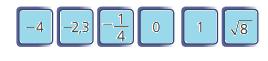
\includegraphics[width=2.79167in,height=0.63542in]{./imgSAEB_8_MAT/media/image1.png}

Inserir uma imagem similar a essa, contendo os mesmos valores

Quais deles pertencem ao conjunto:

a) N

b) Z

c) Z, mas não pertencem a N?

d) Q, mas não pertencem a Z?

Respostas:

a) $0$ ; $1$

b) $-4, 0, 1$

c) $-4$

d) $-2,3$ e $- (\frac{1}{4})$

Em cada item acima deixar o espaço de 1 linha para resposta.

4) observe os números abaixo:

6 $(\sqrt{6}) 6,6 -6$

Inserir uma imagem similar a essa, contendo os mesmos valores.

Identifique quais deles são:

a) reais e naturais.

b) reais e inteiros.

c) reais e racionais.

d) reais e irracionais.

Resposta:

a) $6$

b) $6; -6$

c) $6; -6; 6,6$

d) $(\sqrt{6})$

Em cada item acima deixar o espaço de 1 linha para resposta.

5) Complete os espaços abaixo com pertence ou não pertence:

% Jorge: Que é isso Rogério
a) 100 R*

b) 100 R\textsubscript{+}

c)100 R\textsubscript{-}

d) $(\sqrt{9}) R$

e) $- (\sqrt{9}) R$

f) $(\sqrt{- 9}) R$

g) 2,6 R\textsubscript{+}

Em cada item acima deixar o espaço de 1 linha para resposta.

Respostas:

a) Pertence

b) Pertence

c) Não Pertence

d) Pertence

e) Pertence

f) Não Pertence

g) Pertence

6) A representação decimal de um número pode ser: finita, infinita e
periódica ou, ainda, infinita e não periódica. Escreva qual é o caso de
cada um dos números a seguir

a) $(\frac{15}{6})$

b) $(\frac{1}{3})$

c) $(\sqrt{3})$

d) $(\sqrt{2})$

Em cada item acima deixar o espaço de 1 linha para resposta.

Respostas:

a) Finita

b) infinita e periódica

c) infinita e não periódica

d) infinita e não periódica

7) O número (\pi) é classificado como:

a) um número natural.

b) uma dízima periódica.

c) um número racional.

d) uma dízima não periódica.

Deixar o espaço de 1 linha para resposta.

Resposta: Alternativa D dizima não periódica.

8) Dos números a seguir, qual deles é quadrado perfeito?

a) 170

b) 129

c)121

d) 105

Em cada item acima deixar o espaço de 2 linhas para resposta.

Resposta:

c 121, pois 11 x 11 = 121

9) O produto ou o quociente de dois números irracionais pode ser um
número racional?

Resposta: Sim, como exemplos pode ser citado 
$$(\sqrt{2}) x (\sqrt{2}) = ((\sqrt{2}))^2 = 2$$ 
e também 
$$(\frac{\sqrt{2}}{\sqrt{2}}) = 1$$

deixar o espaço de 3 linhas para resposta.


10) Qual é o menor número natural que devemos multiplicar pelo número
125 para que o produto seja um número quadrado perfeito?

a) 2

b) 3

c) 4

d) 5

Em cada item acima deixar o espaço de 2 linhas para resposta.

Resposta, alternativa D, pois $5 x 125 = 625$ e $(\sqrt{625}) = 25$ logo
um quadrado perfeito.

11) Escreva na forma de fração:

a) 0,57

b) 1,29

c) 3,124

d) -32,40

e) 0,9

f) 0,650

g) 1,342

h) 5,09409

Em cada item acima deixar o espaço de 2 linhas para resposta.

Respostas:

a) $0,57 = (\frac{57}{100})$

b) $1,29 = (\frac{129}{100})$

c) $3,124 = (\frac{3124}{1000})$

% REVER
d) $-32,40 = -(\frac{324}{10})$

e) $0,9 = (\frac{9}{10})$

f) $0,650 = (\frac{65}{100})$

g) $1,342 = (\frac{1342}{1000})$

h) $5,09409 = (\frac{509\ 409}{100\ 000})$

\colorsec{Treino}

1) Qual é a decomposição do número 1 000 em fatores primos?

a) $2^2 x 5^2$

b) $2^3 x 5^2 x 2$

c) $2^3 x 5^3$

d) $2^3x5^2$

Resposta: C

Habilidades Saeb

\begin{itemize}
\tightlist
\item
  Compor ou decompor números racionais positivos (representação decimal
  finita) na forma aditiva, ou em suas ordens, ou em adições e
  multiplicações.
\end{itemize}

A: incorreta ao não computar 1 elemento 2 e um elemento 5 na fatoração
chegará a esse resultado erroneamente.

B: incorreta ao computar 1 elemento 2 a mais e um elemento 5 a menos na
fatoração chegará a esse resultado erroneamente.

C: correta, Ao decompor o número 1 000 em fatores primos obtemos 2³ x 5³

D: incorreta ao não computar 1 elemento 5 na fatoração chegará a esse
resultado erroneamente.

2) Sobre o número 123 456 789, podemos afirmar que:

a) é múltiplo de 5

b) é múltiplo de 2

c) é múltiplo de 3

d) é múltiplo de 10

Resposta: C

Habilidades Saeb

\begin{itemize}
\tightlist
\item
  Identificar um número natural como primo, composto, ``múltiplo/fator
  de'' ou ``divisor de'' ou identificar a decomposição de um número
  natural em fatores primos ou relacionar as propriedades aritméticas
  (primo, composto, ``múltiplo/fator de'' ou ``divisor de'') de um
  número natural à sua decomposição em fatores primos.
\end{itemize}

A: incorreta, o aluno pode realizar a divisão incorretamente do valor
123 456 789 e chegar a essa conclusão ao errar nos cálculos básicos.

B: incorreta, o aluno pode realizar a divisão incorretamente do valor
123 456 789 e chegar a essa conclusão ao errar nos cálculos básicos.

C: Correta, Realizando a soma de $1+2+3+4+5+6+7+8+9=45$ logo $45$ é
múltiplo de 3, então

123 456 789 também será.

D: incorreta, o aluno pode realizar a divisão incorretamente do valor
123 456 789 e chegar a essa conclusão ao errar nos cálculos básicos.

3) Manoel ganhou um prêmio na loteria no valor de R\$ 12 500 345 769, 00
reais, Qual algarismo está situado na casa da centena de milhar?

a)4

b)5

c)0

d)3

Resposta: D

Habilidades Saeb

\begin{itemize}
\tightlist
\item
  Compor ou decompor números racionais positivos (representação decimal
  finita) na forma aditiva, ou em suas ordens, ou em adições e
  multiplicações.
\end{itemize}

A: incorreta: ao contar as casas erroneamente e considerar o número uma
casa a direita o aluno pode considerar esse resultado erroneamente.

Alternativa: B incorreta ao contar as casas erroneamente e considerar o
número duas casas a direita o aluno pode considerar esse resultado
erroneamente.

C: incorreta, ao contar as casas erroneamente e considerar o número uma
casa a esquerda o aluno pode considerar esse resultado erroneamente.

D, Correta o número 3 está situado na casa das centenas de milhar.

\section{Módulo 2}

BNCC: EF08MA01 EF08MA02 EF08MA03

Habilidades Saeb:

Calcular o resultado de adições, subtrações, multiplicações ou divisões
envolvendo número reais.

Calcular o resultado de potenciação ou radiciação envolvendo números
reais.

Resolver problemas de adição, subtração, multiplicação, divisão,
potenciação ou radiciação envolvendo número reais, inclusive notação
científica

Resolver problemas de contagem cuja resolução envolva a aplicação do
princípio multiplicativo.

Resolver problemas que envolvam as ideias de múltiplo, divisor, máximo
divisor comum ou mínimo múltiplo comum.

Potência de um número racional

Dado um número racional a e um número natural n, a expressão
a\textsuperscript{n} chama-se potência e representa uma multiplicação de
n fatores iguais ao número a.

A\textsuperscript{n} =

% REVER
% (\frac{a\ x\ a\ x\ a\ x\ a\ x\ a\ x\ldots x\ a}{n\ \text{fatores}})

Essa operação é chamada potenciação.

Assim, pela definição: temos que

10³ = 10 x 10 x 10 = 1 000

Propriedades da Potenciação:

1a propriedade: Produto de potências de mesma base.

Um produto de potências de mesma base pode ser escrito na forma de uma
única potência: conservamos a base e adicionamos os expoentes.

A\textsuperscript{m} x a\textsuperscript{n} = a\textsuperscript{m+n}

2ª Propriedade: Quociente de potências de mesma base

Um quociente de potências de mesma base, em que o expoente do dividendo
é maior ou igual ao expoente do divisor, pode ser escrito na forma de
uma única potência: conservamos a base e subtraímos os expoentes

$A^{m}$ : $a^{n} = a^{m-n}$,
com a diferente de zero e m maior ou igual a $n$

\begin{comment}

3ª propriedade: Potência de uma potência.

Um produto de potências de mesma base pode ser escrito na forma de uma
única potência: conservamos a base e multiplicamos os expoentes.

(a\textsuperscript{m})\textsuperscript{n} = a^{m~x~n}

4ª propriedade potência de um produto

Para elevar um produto de dois ou mais números racionais a um expoente,
elevamos cada fator a esse expoente.

(a x b)\textsuperscript{n}= a\textsuperscript{n} x b\textsuperscript{n}

Potências de base dez

A potência de base 10, com expoente natural, é uma maneira de se
escrever o número que, no Sistema de Numeração Decimal, é representado
por 1 seguido de n zeros.

10\textsuperscript{5} = 100 000 = 1 + 5 zeros

10³ = 1 000 = 1+ 3 zeros

10^{6} = 1 000 000 = 1+ 6 zeros

Raiz quadrada exata de um número racional não negativo

Se um número representa um produto de dois fatores iguais não negativos,
então cada fator é a raiz quadrada desse número. Por exemplo:

A raiz quadrada de $25$ é $5$, pois $5 x 5 = 52 = 25$. Logo $(\sqrt{25}) = 5$.

A raiz quadrada de $49$ é $7$, pois $7 x 7 = 72 = 49$. Logo $(\sqrt{49}) = 7$.

\colorsec{Atividades}

\[\ \]

1) Calcule o valor das potencias abaixo.

a) $(-\frac{3}{5})^{2}$

b) $( + \frac{1}{2})^{5}$

c) $( - 1\frac{1}{2})^{3}$

d) $(-3,5)^2$

e) ( + \frac{1}{3}))^{0}


% REVER
f) $(-1,5)^1$

Em cada item acima deixar o espaço de 2 linhas para resposta.

Resposta:

a) $(\frac{9}{25})$

b) $(\frac{1}{32})$

c) $(-\frac{3}{8})$

d) +12,25

e) 1

f) -1,5()

2) Calcule as operações abaixo

\textsuperscript{a)~-} (( - \frac{1}{2}))\textsuperscript{²} + (-1)
\textsuperscript{4}


\textsuperscript{b)} -- (2)^3{.} (-2) ³

\textsuperscript{c)} (( - 1\frac{1}{2})) . (-1)\textsuperscript{5}

\textsuperscript{d)}
(\left( - \frac{1}{2} \right).\left( + \frac{3}{2} \right) - \left( \frac{2}{3} \right)^{3}:( - \frac{1}{27})\ )

e) (0,1) ² : (-2) + (1,5)^{.} (-0,1) ²

Em cada item acima deixar o espaço de 2 linhas para resposta.

Respostas:

a) (+ 1\frac{1}{4})

b) +64

c) (+ 1\frac{1}{2})

d) 8(\frac{3}{8})

e) 0,01

3) Use a propriedade e, no caderno, escreva cada quociente como uma
única potência e calcule o valor dela

a) 3\textsuperscript{7}:3\textsuperscript{5}

b)(-1)\textsuperscript{8}:(-1)\textsuperscript{6}

c)(\left( \frac{2}{3} \right):\left( \frac{2}{3} \right))

d) Metade de 2\textsuperscript{10}

e) (-2,5)\textsuperscript{5} : (-2,5)²

f) a\textsuperscript{9}: a\textsuperscript{8} , com a racional não nulo

g) 1\textsuperscript{8}:1²

h) terça parte de 3\textsuperscript{8}

Em cada item acima deixar o espaço de 2 linhas para resposta.

Respostas

a) 3\textsuperscript{7-5}=3² = 3.3= 9

b) (-1)\textsuperscript{8-6}= (-1)²= (-1).(-1)= +1

c)
((\frac{2}{3}))\textsuperscript{4-1}=((\frac{2}{3}))³=((\frac{2}{3})).((\frac{2}{3})).((\frac{2}{3}))=
(\frac{8}{27})

d) 2\textsuperscript{10}: 2¹= 2\textsuperscript{9}= 2.2.2.2.2.2.2.2.2=
572

e) (-2,5)^{5-2} = (-2,5)³= (-2,5). (-2,5). (-2,5)=
-15,625

f) a\textsuperscript{9-8}= a¹ =a

g) 1\textsuperscript{8-2}=1\textsuperscript{6}= 1.1.1.1.1.1=1

h) 3\textsuperscript{8-1}= 3\textsuperscript{7} = 3.3.3.3.3.3.3=2187

4) Jamile fez uma viagem turística ao topo de uma montanha, ao chegar em
certo local observou uma pedra antiga com o seguinte enunciado, esta
pedra tem o peso de {[}(-5)³{]}² kg, quanto pesa a pedra que Jandira
observou?

deixar o espaço de 3 linhas para resposta.

Resposta:

Utilizando a propriedade de multiplicação de expoentes temos que:

(-5)\textsuperscript{3.2}= (-5)\textsuperscript{6}=
(-5)\textsuperscript{.} (-5)\textsuperscript{.} (-5)\textsuperscript{.}
(-5)\textsuperscript{.} (-5)\textsuperscript{.} (-5)= 15 625 kg

5) Uma sala de jantar quadrada terá o piso coberto com ladrilhos com
medida de comprimento dos lados de 60 cm.

a) Qual é a medida de comprimento dos lados da sala sabendo que a medida
de área dela é de 81m²?

b) Quantos ladrilhos serão necessários para cobrir o piso?

Em cada item acima deixar o espaço de 2 linhas para resposta.

Respostas:

a) Considerando que a sala é quadra e que a formula da área de um
quadrado é l ² para descobrirmos o real valor de cada lado, basta
fazermos a operação inversa, no caso a radiciação logo temos que:

l²= 81

l= (\sqrt{81})

l=9

b) Se cada lado da sala possui 9 metros e cada lado do ladrilho possui
0,60 cm temos que:

9:0,6=15

15\textsuperscript{.}15= 225 ladrilhos

6) Utilizando os conhecimentos de redução de potencias, reduza as
potencias abaixo.

a) 10² . 2²

b) 11² . 3²

c) (-6)³^{.} (-8)³

d) (3,1)\textsuperscript{5~.}
(0,7)\textsuperscript{5.}2\textsuperscript{5}

Em cada item acima deixar o espaço de 2 linhas para resposta.

Utilizando o método de redução de potencias temos que

a) (10 . 2) ² = 20 ²

b) (11 . 3) ² = 33²

c) ((-6) . (-8)) ³= 48³

d) (3,1 . 0,7 . 2)^{5}= 4,34\textsuperscript{5}

7) Calcule o valor de cada potência com exponente negativo

a) 8\textsuperscript{-2}

b) 5\textsuperscript{-1}

c)(-2)\textsuperscript{-4}

d)((\frac{1}{2}))\textsuperscript{-3}

e)(-3)\textsuperscript{-3}

f) (\left( \frac{1}{2} \right))\textsuperscript{-5}

Em cada item acima deixar o espaço de 2 linhas para resposta.

Resposta Utilizando a propriedade de expoente negativo da potenciação
temos que:

a) 8\textsuperscript{-2}= (\frac{1}{8²}) = (\frac{1}{64})

b)5\textsuperscript{-1}= (\frac{1}{5¹}) = (\frac{1}{5})

c) (-2)\textsuperscript{-4} = (\frac{1}{2})\textsubscript{4}
=(\frac{1}{16})

d)((\frac{1}{2}))\textsuperscript{-3}= (\frac{2}{1³}) =
(\frac{2}{1}) = 2

e) (-3)\textsuperscript{-3}= (- \frac{1}{3³}) = (\frac{1}{27})

f)(\frac{1}{2})\textsuperscript{-5} =
(\frac{2}{1})\textsubscript{5} = (\frac{2}{1}) = 2

8) Calcule as seguintes potencias de base 10 e coloque as em forma
decimal

a) 10\textsuperscript{6}

b) 10\textsuperscript{-6}

c) 10\textsuperscript{-4}

d)10\textsuperscript{4}

e) 10\textsuperscript{-2}

f) 10^{-5}

g) 10\textsuperscript{10}

h) 10\textsuperscript{-8}

Em cada item acima deixar o espaço de 2 linhas para resposta.

Respostas:

a) 1 000 000

b) 0, 000 001

c) 0, 0001

d) 10 000

e) 0,01

f) 0,00001

g) 10 000 000 000

h) 0,00000001

9) Reinaldo é professor, e durante uma de suas de estatística resolveu
demonstrar a população da terra em formato decimal, porem ao tentar
fazer a demonstração acabou que o espaço de sua lousa não foi
suficiente, Sabendo que a população da terra em 2022 chegou em 8
bilhões, como poderia ser representado este mesmo número para que caiba
na lousa?

Deixar o espaço de 3 linhas para resposta.

Resposta:

Reinaldo poderia representar por meio de Notação cientifica (potência de
base 10)

Considerando a população da terra como 8 000 000 000 outra forma de
reescrever seria

8^{.} 10\textsuperscript{9} sendo assim ocupando um
menor espaço.

10) Felipe é artista e uma de suas obras é conhecida como quadrado
infinito ao observar o quadro um matemático fez as seguintes descobertas

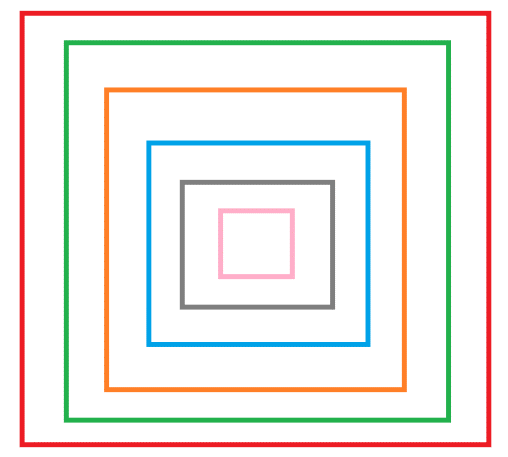
\includegraphics[width=2.3125in,height=2.07917in]{./imgSAEB_8_MAT/media/image2.png}

O quadrado Vermelho possui uma área de 256 cm²

O quadrado Verde possui uma área de 225 cm²

O quadrado Laranja possui uma área de 144 cm²

O quadrado Azul possui uma área de 64 cm²

O quadrado Cinza possui uma área de 36 cm²

O quadrado Rosa possui uma área de 16 cm²

Com as informações obtidas pelo matemático podemos afirmar que os
perímetros das respectivas figuras são:

a) Perímetro do quadrado vermelho

b) Perímetro do quadrado verde

c) Perímetro do quadrado laranja

d) Perímetro do quadrado azul

e) Perímetro do quadrado cinza

f) Perímetro do quadrado rosa

Em cada item acima deixar o espaço de 3 linhas para resposta.

Respostas:

Para descobrir o perímetro de cada quadrado a solução se mostra a mesma
se temos que a formula da área de um quadrado é l ² para descobrirmos o
real valor de cada lado, basta fazermos a operação inversa, no caso a
radiciação.

a)(\sqrt{256})= 16, 16^{.} 4 = perímetro= 64

b)(\sqrt{225}) = 15, 15\textsuperscript{.}4 = perímetro = 60

c)(\sqrt{144}) = 12, 12\textsuperscript{.}4= perímetro= 48

d)(\sqrt{64})= 8, 8\textsuperscript{.}4= perímetro 32

e)(\sqrt{36})= 6, 6\textsuperscript{.}4=perímetro= 24

f)(\sqrt{16})= 4, 4\textsuperscript{.}4=perímetro =16

\colorsec{Treino}

1) Raul estava passeando pela rua e ao passar por uma loja de discos
antigos viu um álbum musical com o seguinte título: ``Eu Nasci Há Dez
Mil Anos Atrás'', se a capa desse álbum fosse representada em forma de
potência de base 10 qual o novo nome do álbum?

a) Eu Nasci Há 10² anos Atrás

b) Eu Nasci Há 10³ anos atrás

c) Eu Nasci Há 10\textsuperscript{4} anos atrás

d) Eu Nasci Há 10\textsuperscript{5} Anos Atrás

Resposta: C

BNCC: EF09MA01

Habilidade Saeb:

Resolver problemas de adição, subtração, multiplicação, divisão,
potenciação ou radiciação envolvendo número reais, inclusive notação
científica

A, incorreta, ao considerar o número de ``zeros'' incorretamente ao
invés de 4 zeros consideráveis para 2, ocorreria esse erro.

B, incorreta, ao considerar o número de ``zeros'' incorretamente ao
invés de 4 zeros consideráveis para 3, ocorreria esse erro.

C, Correta pois:

10000 =
10\textsuperscript{.}10\textsuperscript{.}10\textsuperscript{.}10 ou
seja 10\textsuperscript{4}

D, incorreta, ao considerar o número de ``zeros'' incorretamente ao
invés de 4 zeros consideráveis para 5, ocorreria esse erro.

2) Thiago é um professor de matemática e ao comemorar seu aniversário
com seus alunos resolveu lançar um enigma, sua idade seria o expoente do
resultado da seguinte expressão:

2\textsuperscript{25.}2\textsuperscript{35.}2\textsuperscript{30}

2\textsuperscript{2.}2\textsuperscript{1}

Qual a Idade de Thiago?

a) 2

b) 93

c) 45

d) 30

Resposta: D

BNCC: EF09MA01

Habilidade Saeb:

Resolver problemas de adição, subtração, multiplicação, divisão,
potenciação ou radiciação envolvendo número reais, inclusive notação
científica

A: incorreta, ao confundir expoente com base chegaria a esse resultado
erroneamente.

B: incorreta: o aluno chegaria a esse conclusão se somasse todos os
expoentes incorretamente.

C: incorreta, pois ao dividir o expoente do numerado por 2 ao invés de
3, o aluno chegaria a esse resultado.

D: Correta pois, utilizando a propriedade de multiplicação e divisão de
potencias de mesma base temos que

No numerador 2\textsuperscript{25+35+30}=2\textsuperscript{90}

No denominador 2\textsuperscript{2+1}=2³

Realizando a divisão temos que
2\textsuperscript{90:3}=2\textsuperscript{30}

Considerando que a idade de Thiago é apenas o expoente temos que Thiago
tem 30 anos.

3) Um pen drive possui diferentes capacidades de memória, mas a medida
normalmente utilizada é o GB, sabendo que 1 GB = 2\textsuperscript{10}
megabytes, ao comprar um pen drive de 32 GB quantos megabytes
disponíveis de armazenamento estará disponível?

a) 32 768 megabytes

b) 32 000 megabytes

c) 16 384 megabytes

d) 64 megabytes

Resposta: A

BNCC: EF09MA01

Habilidade Saeb:

Resolver problemas de adição, subtração, multiplicação, divisão,
potenciação ou radiciação envolvendo número reais, inclusive notação
científica.

A:Correta pois:

2\textsuperscript{10} = 1024

1024^{.}32= 32768 megabytes.

B: incorreta, o aluno chegaria a esse resultado erroneamente ao
considerar que 2\textsuperscript{10} seja 1 000 ao invés de 1 024.

C: incorreta, ao considerar um ``dois'' a menos na expressão, chegaria a
esse resultado incorreto.

D: incorreta, ao realizar apenas a multiplicação ao invés de realizar o
cálculo da potência o aluno chegaria a esse resultado erroneamente.

\section{Módulo 3}

BNCC: EF08MA051

Habilidades Saeb:

\begin{itemize}
\item
  Representar frações menores ou maiores que a unidade por meio de
  representações pictóricas ou associar frações a representações
  pictóricas.
\item
  Identificar frações equivalentes.
\item
  Determinar uma fração geratriz para uma dízima periódica.
\end{itemize}

Comparação de números racionais

Comparar dois números racionais significa dizer se um é maior que o
outro, ou se é menor ou, ainda, se é igual.

Todo número racional negativo é menor que todo número racional positivo

\begin{itemize}
\tightlist
\item
  (\frac{1}{5}) \textless{} (\frac{3}{4})
\end{itemize}

Todo número racional negativo é menor que zero

-5 \textless{} 0 -12,5 \textless{} 0 -(\frac{3}{2}) \textless{} 0

Operações com números racionais

Adição e subtração

Na forma fracionária Temos que estudar dois casos distintos: o primeiro
deles refere-se às frações com denominadores iguais.

O segundo, às frações com denominadores diferentes.

1° caso: Frações de mesmo denominador. Para somarmos (ou subtrairmos)
frações de mesmo denominador, mantemos o denominador e somamos (ou
subtraímos) os numeradores. Veja um exemplo:

(\frac{3}{5}) + (\frac{6}{5}) = (\frac{9}{5})

2° caso: Frações com denominadores diferentes. Para somarmos (ou
subtrairmos) frações com denominadores diferentes, devemos obter frações
equivalentes às frações dadas, de mesmo denominador. Em seguida,
mantemos o denominador comum e somamos (ou subtraímos) os numeradores.

(\frac{2}{4}) + (\frac{3}{7}) = (\frac{14 + 12}{28}) =
(\frac{26}{28})

Multiplicação de números racionais

Na forma fracionária Para multiplicarmos dois números racionais na forma
fracionária, multiplicamos os numeradores entre si e, em seguida, os
denominadores. Caso seja necessário, simplificamos o resultado até obter
a fração irredutível. Exemplo:

(\frac{3}{4}) x (\frac{2}{5}) = (\frac{6}{20})= (\frac{3}{10})

Divisão de números racionais

Na forma fracionária Para dividirmos dois números racionais na forma
fracionária, mantemos a primeira fração e multiplicamos pelo inverso da
segunda.

(\frac{1}{2}) : (\frac{3}{5})= (\frac{1}{2}) x (\frac{5}{3}) =
(\frac{5}{6})

Dízimas periódicas

Em Matemática, muitas vezes, é útil representar números racionais,
expressos por meio de frações, na forma decimal. Para isso, basta
dividir o numerador pelo denominador. Em alguns casos, essa
representação decimal é finita em outros casos essa representação
decimal é infinita. Exemplo:

(\frac{1}{3}) = 0,3333333......

Fração geratriz de dízimas periódicas simples

Vamos encontrar a fração geratriz da dízima periódica 0,333333 ..., ou
seja, encontrar qual fração, quando transformada em número racional na
forma decimal, gera essa dízima.

Para isso, montamos uma equação:

0,333333333...-\/-\/-\/-\/-\/-\/-\/-\/-\/-\/-\/-\/-\/-x

3,33333333...-\/-\/-\/-\/-\/-\/-\/-\/-\/-\/-\/-\/-\/- 10x

3,3333333333... -- 0,333333333... = 3

10 x -- x = 9x

Logo temos que (\frac{3}{9}) simplificando (\frac{1}{3}) é a nossa
fração geratriz.

\colorsec{Atividades}

1) Classifique com V para verdadeiro e F para falso as afirmações a
seguir:

( ) 4,9 = 4,09

( ) -15,3 \textless{} 15,3

( ) (\frac{19}{3}) \textgreater{} (\frac{23}{3})

( )- (\frac{89}{7}) \textless{} (- \frac{63}{4})

( )(- \frac{7}{5}) \textgreater{} -1,4

( ) 23,98 \textgreater{} 23,89

Em cada item acima deixar o espaço de 1 linha para resposta.

Respostas:

( F ) 4,9 = 4,09

( V ) -15,3 \textless{} 15,3

( F ) (\frac{19}{3}) \textgreater{} (\frac{23}{3})

( V )- (\frac{89}{7}) \textless{} (- \frac{63}{4})

( F )(- \frac{7}{5}) \textgreater{} -1,4

( V) 23,98 \textgreater{} 23,89

2) Efetue as operações a seguir:

a)(- \frac{8}{5}) + 2,5 =

b) (\frac{14}{3}) + (\frac{19}{5})

c) -(\frac{8}{13}) - (\frac{3}{5})

d) 79,02 -- (\frac{12}{5})

e) 125 - (\frac{35}{4})

f) (\frac{49}{7}) + (\frac{2}{3})

g) 50 - (\frac{1}{2})

h) 100 - (\frac{1}{3})

Em cada item acima deixar o espaço de 2 linhas para resposta.

Respostas:

a)(- \frac{8}{5}) + 2,5 = -(\frac{8}{5}) + (\frac{25}{10}) =
(\frac{- 16}{10})+(\frac{25}{10}) = (\frac{9}{10})

b) (\frac{14}{3}) + (\frac{19}{5})= (\frac{70}{15}) +
(\frac{57}{15}) = (\frac{127}{15})

c)- (\frac{8}{13}) - (\frac{3}{5}) = (- \frac{40}{65}) -
(\frac{39}{65}) = - (\frac{79}{65})

d) 79,02 -- (\frac{12}{5}) = (\frac{7\ 902}{100}) - (\frac{12}{5})
= (\frac{7\ 902}{100}) - (\frac{240}{100}) = (\frac{7\ 662}{100})

e) 125 - (\frac{35}{4}) = (\frac{125}{1}) - (\frac{35}{4}) =
(\frac{500}{4}) - (\frac{35}{4}) = (\frac{465}{4})

f) (\frac{49}{7}) + (\frac{2}{3}) = (\frac{147}{21}) +
(\frac{14}{21}) = (\frac{161}{21})

g) 50 - (\frac{1}{2}) = (\frac{50}{1}) - (\frac{1}{2}) =
(\frac{100}{2}) - (\frac{1}{2}) = (\frac{99}{2})

h) 100 - (\frac{1}{3}) = (\frac{100}{1}) - (\frac{1}{3}) =
(\frac{300}{3}) - (\frac{1}{3}) = (\frac{299}{3})

3) Resolva as multiplicações abaixo, mas antes de calcular transforme os
decimais em fracionários

a) 0,5 . 12,7

b) 3,6 . 6,7

c) 9,3 . 13,25

d) 2,9 . 3,8

e) 11,2 . 4,2

f) 7,5 . 6,6

g) 0,456 . 0,345

h) 0,01 . 0,001

Em cada item acima deixar o espaço de 2 linhas para resposta.

Respostas:

a) 0,5 . 12,7 = (\frac{5}{10}) . (\frac{127}{10}) =
(\frac{635}{100})

b) 3,6 . 6,7 = (\frac{35}{10}) . (\frac{67}{10})

c) 9,3 . 13,25 = (\frac{93}{10}) . (\frac{1325}{100}) =
(\frac{123\ 225}{1\ 000})

d) 2,9 . 3,8 = (\frac{29}{10}) . (\frac{38}{10}) =
(\frac{1102}{100})

e) 11,2 . 4,2= (\frac{112}{10}) . (\frac{42}{10}) =
(\frac{4\ 704}{100})

f) 7,5 . 6,6 = (\frac{75}{10}) . (\frac{66}{10}) =
(\frac{4950}{100})

g) 0,456 . 0,345 = (\frac{456}{1\ 000}) . (\frac{345}{1\ 000}) =
(\frac{157\ 320}{1\ 000\ 000})

h) 0,01 . 0,001= (\frac{1}{100}) . (\frac{1}{1\ 000}) =
(\frac{1}{100\ 000})

4) Resolva as Divisões abaixo, mas antes transforme os decimais em
fracionários

a) 0,5 : 3,4

b) 9,4 : 3,1

c) 5,1 : 0,2

d) 0,2 : 0,1

e) 0,01 : 0,001

f) 2,1 : 0,5

g) 4,2 : 0,1

h) 3,1: 1,5

Em cada item acima deixar o espaço de 2 linhas para resposta.

Respostas:

a) 0,5 : 3,4 = (\frac{5}{10}) : (\frac{34}{10}) = (\frac{5}{10}) .
(\frac{10}{34}) = (\frac{50}{340})

b) 9,4 : 3,1 = (\frac{94}{10}) : (\frac{31}{10}) = (\frac{94}{10})
. (\frac{10}{31}) = (\frac{940}{310})

c) 5,1 : 0,2 = (\frac{51}{10}) : (\frac{2}{10}) = (\frac{51}{10})
. (\frac{10}{2}) = (\frac{510}{20})

d) 0,2 : 0,1 = (\frac{2}{10}) : (\frac{1}{10}) = (\frac{2}{10}) .
(\frac{10}{1}) = (\frac{20}{10}) = 2

e) 0,01 : 0,001= (\frac{1}{100}) : (\frac{1}{1\ 000}) =
(\frac{1}{100}) . (\frac{1\ 000}{1}) = (\frac{1\ 000}{100}) = 10

f) 2,1 : 0,5 = (\frac{21}{10}) : (\frac{5}{10}) = (\frac{21}{10})
. (\frac{10}{5}) = (\frac{210}{50})

g) 4,2 : 0,1= (\frac{42}{10}) : (\frac{1}{10}) = (\frac{42}{10}) .
(\frac{10}{1})= (\frac{420}{10}) = 42

h) 3,1: 1,5 = (\frac{31}{10}) : (\frac{15}{10}) = (\frac{31}{10})
. (\frac{10}{15}) = (\frac{310}{150})

5) Transforme as dizimas periódicas abaixo em frações geratrizes:

a) 2,333333...

b) 3,181818...

c) 0,144444...

d) 4,166666...

e) 1,2222...

Em cada item acima deixar o espaço de 4 linhas para resposta.

Respostas:

a) 2,333333...

23,333333...
-\/-\/-\/-\/-\/-\/-\/-\/-\/-\/-\/-\/-\/-\/-\/-\/-\/-\/-\/-\/-\/-\/-\/-\/-\/-\/-\/-
10x

2,3333333...
-\/-\/-\/-\/-\/-\/-\/-\/-\/-\/-\/-\/-\/-\/-\/-\/-\/-\/-\/-\/-\/-\/-\/-\/-\/-\/-\/-
x

23,33333... - 2,3333333... = 21

10x -- x = 9x

Logo (\frac{21}{9}) = (\frac{7}{3})

b) 3,181818...

318,1818...
-\/-\/-\/-\/-\/-\/-\/-\/-\/-\/-\/-\/-\/-\/-\/-\/-\/-\/-\/-100x

3,181818...
-\/-\/-\/-\/-\/-\/-\/-\/-\/-\/-\/-\/-\/-\/-\/-\/-\/-\/-\/-\/-x

318,1818... -- 3,181818... = 315

100 x -- x = 99x

Logo= (\frac{315}{99})

c) 0,144444...

1,444444... -\/-\/-\/-\/-\/-\/-\/-\/-\/-\/-\/-\/-\/-\/-\/-\/-\/-\/- 10x

14,444444... -\/-\/-\/-\/-\/-\/-\/-\/-\/-\/-\/-\/-\/-\/-\/-\/-\/-\/-
100x

14,4444444 -- 1,44444444 = 13

100x -10x = 90x

Logo (\frac{13}{90})

d) 4,166666...

41, 666666...
-\/-\/-\/-\/-\/-\/-\/-\/-\/-\/-\/-\/-\/-\/-\/-\/-\/-\/-\/-\/-\/-\/-\/-\/-\/-
10x

416,66666...
-\/-\/-\/-\/-\/-\/-\/-\/-\/-\/-\/-\/-\/-\/-\/-\/-\/-\/-\/-\/-\/-\/-\/-\/-\/-\/-
100x

416,666666 -- 41,6666666 = 375

100 x -- 10 x = 90x

Logo = (\frac{375}{90}) = (\frac{25}{6})

e) 1,2222...

1,222222 -\/-\/-\/-\/-\/-\/-\/-\/-\/-\/-\/-\/-\/-\/-\/- x

12,22222 -\/-\/-\/-\/-\/-\/-\/-\/-\/-\/-\/-\/-\/-\/-\/- 10x

12,222222 -- 1,2222222 = 11

10x -- x = 9

Logo: (\frac{11}{9})

6) Prove que 0,99999999999999 = 1

Deixar o espaço de 4 linhas para resposta.

Resposta:

0,99999999 -\/-\/-\/-\/-\/-\/-\/-\/-\/-\/-\/-\/-\/-\/-\/-\/-\/-\/-\/- x

9,99999999 -\/-\/-\/-\/-\/-\/-\/-\/-\/-\/-\/-\/-\/-\/-\/-\/-\/-\/-\/-
10x

9,999999999 -- 0,999999999 = 9

10 x -- x = 9

Logo (\frac{9}{9}) = 1

7) Complete com X as lacunas corresponde aos valores corretos

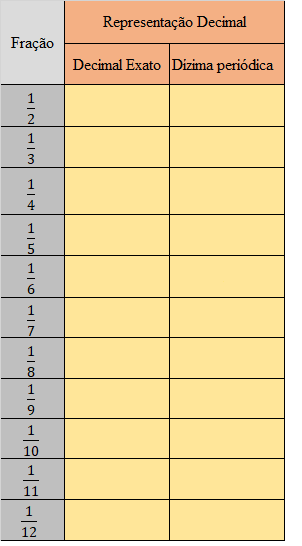
\includegraphics[width=2.37378in,height=4.29167in]{./imgSAEB_8_MAT/media/image3.png}

Inserir uma tabela similar a essa, contendo os mesmos valores, as cores
podem ser modificadas.

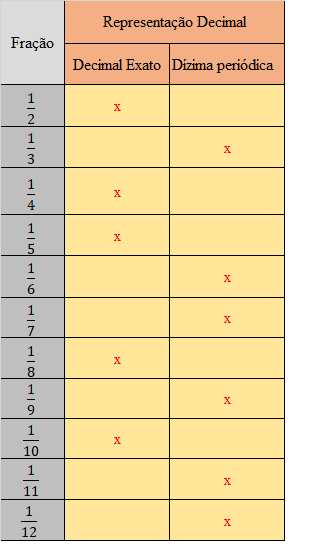
\includegraphics[width=2.14722in,height=3.775in]{./imgSAEB_8_MAT/media/image4.png}

Respostas:

8) Juliana está realizando suas atividades extracurriculares, ao
realizar 2 operações na calculadora obteve os seguintes resultados:
3,33333333... e 0,8888888...

Quais operações Juliana pode ter realizado?

Deixar o espaço de 4 linhas para resposta.

Respostas:

1° caso

3,333333333
-\/-\/-\/-\/-\/-\/-\/-\/-\/-\/-\/-\/-\/-\/-\/-\/-\/-\/-\/-\/- x

33,33333333 -\/-\/-\/-\/-\/-\/-\/-\/-\/-\/-\/-\/-\/-\/-\/-\/-\/-\/-\/-
10 x

33,33333333... -- 3,33333333... = 30

10 x -- x = 9

Logo temos que Juliana Realizou a operação (\frac{30}{9}) ou frações
equivalentes a essa como operação

Analogamente temos que

0,888888888-\/-\/-\/-\/-\/-\/-\/-\/-\/-\/-\/-\/-\/-\/-\/-\/-\/-\/-\/-\/-
x

8,888888888 -\/-\/-\/-\/-\/-\/-\/-\/-\/-\/-\/-\/-\/-\/-\/-\/-\/-\/-\/-
10 x

8,8888888... -- 0,88888888 = 8

10x-x = 9

Logo temos que Juliana Realizou a operação (\frac{8}{9}) ou frações
equivalentes a essa como operação.

9) Um professor de matemática aposentado resolveu inovar em sua festa de
aniversário, na parede do salão de festas colocou um cartaz com os
seguintes dizeres ``ao descobrirem a fração geratriz do número
5,454545..., saberão que o numerador desta fração é a idade que estou
completando hoje'' Quantos anos o professor está completando?

a) 50 anos

b) 52 anos

c) 56 anos

d) 60 anos

Deixar o espaço de 4 linhas para resposta.

Resposta:

5,45454545...-\/-\/-\/-\/-\/-\/-\/-\/-\/-\/-\/-\/-\/-\/-\/-\/-\/-\/-\/-\/-
x

545,454545... -\/-\/-\/-\/-\/-\/-\/-\/-\/-\/-\/-\/-\/-\/-\/-\/-\/-\/-\/-
100 x

5,45454545... -- 545,454545 = 540

100 -- x = 99

Logo temos que (\frac{540}{99}) = (\frac{60}{11}) logo 60 anos

10) Marly e Marla são irmãs gêmeas e ao divirem tarefas domésticas
decidiram que cada uma ia limpar uma parte da casa, desde que ambas
limpassem ao final a mesma fração que a outra, Sabendo que Marly limpou
(\frac{3}{9}) da casa, Qual fração da casa Marla deverá limpar da casa
?

a)(\frac{6}{18})

b) (\frac{2}{3})

c) (\frac{5}{9})

d) (\frac{1}{4})

Deixar o espaço de 3 linhas para resposta.

\colorsec{Treino}

1) Assinale a alternativa correta:

a) O valor do número (\pi) que é aproximadamente
3,14159265358979323846\ldots{} é considerado uma dizima periódica
simples pois seus 3 últimos números da sequência são pares

b) o número de ouro representado pelo número 1.61803399... é considerado
uma dizima periódica simples

c) Ao calcularmos uma dizima periódica simples, sempre encontramos uma
fração geratriz

d) O Conjunto dos números irracionais são compostos por dizimas
periódicas simples.

Resposta: C

BNCC: EF08MA05

Habilidade Saeb:

Determinar uma fração geratriz para uma dízima periódica.

A: incorreta, o aluno pode ter uma confusão conceitual passando a
acreditar que o número (\pi) seja de fato uma dizima periódica simples
pelo fato de ter números pares na sua composição.

B: incorreta, o aluno pode ter uma confusão conceitual ao não conseguir
identificar uma a diferença entre uma dizima periódica simples e um
irracional.

C, Correta. Questão conceitual.

D, incorreta, o aluno pode ter uma confusão conceitual ao não conseguir
identificar uma a diferença entre uma dizima periódica simples e um
irracional.

2) Ao realizar uma palestra um renomado medico descobriu que apenas
(\frac{2}{3}) considerou boa a palestra e do restante (\frac{1}{6})
considerou a palestra péssima, qual foi a fração corresponde aos que
acharam a palestra péssima?

a)(\frac{5}{6})

b)(\frac{2}{18})

c) (\frac{12}{3})

d)(\frac{1}{18})

BNCC: EF08MA05

Habilidade Saeb: Representar frações menores ou maiores que a unidade
por meio de representações pictóricas ou associar frações a
representações pictóricas.

A: incorreta, o aluno chegaria a esse resultado caso realizasse a soma
de ambos os termos do enunciado.

B: incorreta, o aluno chegaria a esse valor caso multiplicasse os
valores do enunciado.

C:incorreta, o aluno chegaria a esse valor caso dividisse os valores do
enunciado.

D:Correta, pois

Considerando que (\frac{1}{3}) não gostou ou 0,333333333... Retirando
(\frac{1}{6}) obtemos 0,0555555.\ldots{}

Logo

55,55555555... -\/-\/-\/-\/-\/-\/-\/-\/-\/-\/-\/-\/-\/-\/- 1000 x

5,555555555.\ldots{} -\/-\/-\/-\/-\/-\/-\/-\/-\/-\/-\/-\/-\/-\/- 100x

55,555555.\ldots. -- 5,5555555.\ldots{} = 50

1000x -- 100x = 900

Logo temos (\frac{50}{900}) dividindo numerador e denominador por 50
temos (\frac{1}{18})

3) Ao Fazer um bolo de aniversário, Cecilia utiliza 400 g de farinha de
trigo, ao dividir este bolo em 22 pedaços, Qual fração geratriz
representara a quantidade de farinha em cada pedaço de bolo?

a)(\frac{200}{1})

b) (\frac{1\ 000}{99})

c)(\frac{200}{9})

d) (\frac{1\ 800}{101})

Resposta: C

BNCC: EF08MA05

Habilidade Saeb: Determinar uma fração geratriz para uma dízima
periódica.

A: incorreta, o aluno pode chegar a esse valor ao calcular erroneamente
a expressão e ao invés de calcular 1 800 : 99 , calcular 1 800 : 9

B: incorreta, o aluno pode chegar a esse valor ao calcular erroneamente
a expressão e ao invés de calcular 1 800 : 99 , calcular 1 000 : 9

C: Correta, pois: 400 g : 22 pedaços = 18,1818181818.\ldots{}

18,181818181818...
-\/-\/-\/-\/-\/-\/-\/-\/-\/-\/-\/-\/-\/-\/-\/-\/-\/-\/-\/- x

1818,18181818...
-\/-\/-\/-\/-\/-\/-\/-\/-\/-\/-\/-\/-\/-\/-\/-\/-\/-\/-\/-\/-\/-\/-100x

1818,181818.\ldots{} -- 18,18181818... = 1800

100x -- x = 99x

Logo temos (\frac{1\ 800}{99}) dividindo ambos por 9 temos que
(\frac{200}{9})

D : incorreta, o aluno pode chegar a esse valor ao calcular erroneamente
a expressão e ao invés de calcular 1 800 : 99 , calcular 1 800 : 101

\section{Módulo 4}

BNCC: EF08MA04

Habilidade Saeb:

\begin{itemize}
\tightlist
\item
  Resolver problemas que envolvam porcentagens, incluindo os que lidam
  com acréscimos e decréscimos simples, aplicação de percentuais
  sucessivos e determinação de taxas percentuais.
\end{itemize}

Porcentagem

Porcentagem é a divisão por cem de algo a ser calculado.

Exemplo:

30 \% de uma jarra de suco

40\% de uma barra de chocolate

25 \% de água de um balde

Para calcular, existem duas formas, ou pelo método da regra de 3
simples, ou pelo método multiplicativo de seu corresponde decimal.

Exemplo:

25\% de 300

Pelo método da regra de três simples temos:

100\% -\/-\/-\/-\/-\/-\/-\/-\/-\/-\/-\/- 300

25\% -\/-\/-\/-\/-\/-\/-\/-\/-\/-\/-\/-\/-\/-\/- x

100 x = 25 . 300

100x = 7500

X = 75

Pelo método multiplicativo de seu correspondente decimal temos:

300 . (\frac{25}{100}) = 75

\colorsec{Atividades}

1) Em uma gincana realizada por uma escola haverá várias modalidades
para que os alunos se inscrevam para participar. Ao final das inscrições
30 alunos escolheram jogar futsal, 18 alunos escolheram jogar Vôlei, 45
alunos escolheram jogar basquete e 32 alunos escolheram não participar
de nenhuma modalidade.

Calcule então:

a) \% dos alunos que escolheram jogar futsal

b) \% dos alunos que escolheram jogar vôlei

c) \% dos alunos que escolheram jogar basquete

d) \% dos alunos que escolheram não participar de nenhuma modalidade

Em cada item acima deixar o espaço de 3 linhas para resposta.

Respostas:

Sabendo que o total de alunos é 125 temos que

a) futsal

125-\/-\/-\/-\/-\/-\/-\/-\/-\/-\/-\/-\/-\/-\/-\/-\/-\/-\/-\/-\/-\/-100

30 -\/-\/-\/-\/-\/-\/-\/-\/-\/-\/-\/-\/-\/-\/-\/-\/-\/-\/-\/-\/-\/-\/- x

125 . x = 30 . 100

125x= 3000

X= 24 \%

b) Vôlei

125-\/-\/-\/-\/-\/-\/-\/-\/-\/-\/-\/-\/-\/-\/-\/-\/-\/-\/-\/-\/-\/-100

18-\/-\/-\/-\/-\/-\/-\/-\/-\/-\/-\/-\/-\/-\/-\/-\/-\/-\/-\/-\/-\/-\/- x

125 . x = 100 . 18

125x = 1800

X = 14,4\%

c) basquete

125-\/-\/-\/-\/-\/-\/-\/-\/-\/-\/-\/-\/-\/-\/-\/-\/-\/-\/-\/-\/-\/-100

45-\/-\/-\/-\/-\/-\/-\/-\/-\/-\/-\/-\/-\/-\/-\/-\/-\/-\/-\/-\/-\/-\/-\/-
x

125 x = 4500

X = 36\%

d) nenhuma das modalidades.

125-\/-\/-\/-\/-\/-\/-\/-\/-\/-\/-\/-\/-\/-\/-\/-\/-\/-\/-\/-\/-\/-100

32-\/-\/-\/-\/-\/-\/-\/-\/-\/-\/-\/-\/-\/-\/-\/-\/-\/-\/-\/-\/-\/-\/-\/-
x

125 . x = 32 . 100

125x = 3200

X = 25,6

2) Marcos é corretor de imóveis, em janeiro após ter um grande sucesso
em suas vendas recebeu um aumento de 10\% no salário que passou a ser de
R\$ 2 178,00. O valor do salário de Marcos antes do aumento era:

a) 1980

b) 1990

c) 2000

d) 2100

Deixar o espaço de 3 linhas para resposta.

Resposta:

Utilizando a regra de 3 simples temos que:

X-\/-\/-\/-\/-\/-\/-\/-\/-\/-\/-\/-\/-\/-\/-\/-\/-\/-\/-\/-\/-\/-100

2178-\/-\/-\/-\/-\/-\/-\/-\/-\/-\/-\/-\/-\/-\/-\/-\/-\/-\/-\/-\/-\/-\/-\/-110

Logo x. 110 = 2178 . 100

110x = 217 800

X= 1980

3) Após uma apresentação de teatro, 250 espectadores foram entrevistados
e opinaram sobre o show. Veja o resultado dessa pesquisa:

\begin{itemize}
\item
  Ótimo = 105
\item
  Bom = 100
\item
  Regular = 30
\item
  Ruim =15
\end{itemize}

Calcule a \% de cada opinião:

Em cada item acima deixar o espaço de 3 linhas para resposta.

Respostas:

Ótimo

250-\/-\/-\/-\/-\/-\/-\/-\/-\/-\/-\/-\/-\/-\/-\/-\/-\/-\/-\/-\/-\/-100

105-\/-\/-\/-\/-\/-\/-\/-\/-\/-\/-\/-\/-\/-\/-\/-\/-\/-\/-\/-\/-\/-\/-\/-
x

250 . x = 100 . 105

250x = 10 500

X = 42\%

Bom

250-\/-\/-\/-\/-\/-\/-\/-\/-\/-\/-\/-\/-\/-\/-\/-\/-\/-\/-\/-\/-\/-100

100-\/-\/-\/-\/-\/-\/-\/-\/-\/-\/-\/-\/-\/-\/-\/-\/-\/-\/-\/-\/-\/-\/- x

250 . x = 100 . 100

250x= 10 000

X= 40 \%

Regular

250-\/-\/-\/-\/-\/-\/-\/-\/-\/-\/-\/-\/-\/-\/-\/-\/-\/-\/-\/-\/-\/-100

30-\/-\/-\/-\/-\/-\/-\/-\/-\/-\/-\/-\/-\/-\/-\/-\/-\/-\/-\/-\/-\/-\/-\/-
x

250.x=100 .30

250x = 3000

X = 12 \%

250-\/-\/-\/-\/-\/-\/-\/-\/-\/-\/-\/-\/-\/-\/-\/-\/-\/-\/-\/-\/-\/-100

15-\/-\/-\/-\/-\/-\/-\/-\/-\/-\/-\/-\/-\/-\/-\/-\/-\/-\/-\/-\/-\/-\/-\/-
x

250x = 100 . 15

250 x = 1500

X = 6 \%

4) Valdemar é mecânico e adquiriu um carro quebrado pelo valor de R\$ 10
000,00, depois que arrumou o carro resolveu vendê-lo. Ele anunciou o
carro pelo valor de R\$ 16 000,00. Qual é o fator multiplicativo que ele
utilizou?

a) 0,2

b) 0,4

c) 0,5

d) 0,6

Deixar o espaço de 3 linhas para resposta.

Resposta:

Utilizando a regra de 3 simples temos que:

10 000
-\/-\/-\/-\/-\/-\/-\/-\/-\/-\/-\/-\/-\/-\/-\/-\/-\/-\/-\/-\/-\/-100

16 000
-\/-\/-\/-\/-\/-\/-\/-\/-\/-\/-\/-\/-\/-\/-\/-\/-\/-\/-\/-\/-\/-\/-\/-x

Logo 10 000 . x = 16 000 . 1000

10 000 x = 1 600 000

X = 160

Logo houve um acréscimo de 60\% então 60 : 100= 0,6

O fator multiplicativo foi de 0,6

5) Amanda trabalha em uma loja de calçados, certo dia seu gerente
ofereceu uma \% fixa de comissão para cada funcionário, se na venda de
um tênis de 150 reais, Amanda obteve uma comissão de 12 reais. Qual \%
fixa Amanda ganhará sobre cada produto?

a) 6\%

b) 8\%

c) 10\%

d) 12\%

Deixar o espaço de 3 linhas para resposta.

Resposta:

Utilizando a regra de 3 simples temos que:

150 -\/-\/-\/-\/-\/-\/-\/-\/-\/-\/-\/-\/-\/-\/-\/-\/-\/-\/-\/-\/-\/-100

12
-\/-\/-\/-\/-\/-\/-\/-\/-\/-\/-\/-\/-\/-\/-\/-\/-\/-\/-\/-\/-\/-\/-\/-x

Logo 150 . x = 12 . 100

150 x = 1200

X = 8 \%

6) Em uma pesquisa realizada em um colégio obteve se que nesse colégio
estudam 3 200 alunos, dos quais 1440 são meninos. O número de meninas
representa quantos por cento do total de alunos que estudam nesse
colégio?

Deixar o espaço de 3linhas para resposta.

Resposta:

Utilizando a regra de 3 simples temos que:

3200-\/-\/-\/-\/-\/-\/-\/-\/-\/-\/-\/-\/-\/-\/-\/-\/-\/-\/-\/-\/-\/-100

1440
-\/-\/-\/-\/-\/-\/-\/-\/-\/-\/-\/-\/-\/-\/-\/-\/-\/-\/-\/-\/-\/-\/-\/-x

Logo, 3200 . x = 1440 . 100

3200x = 144 000

X = 45\% de meninos

Logo 55\% são meninas

7) . Magda está tendo aulas na auto escola de sua cidade, ao terminar o
curso Magda realizou uma prova escrita contendo leis de transito, Magda
acertou 38 das 50 questões da prova, sabendo que para passar na prova
escrita Magda precisava acertar pelo menos 80\% da prova, ela foi
aprovada ou reprovada?

Deixar o espaço de 3linhas para resposta.

Resposta:

Utilizando a regra de 3 simples temos que:

50-\/-\/-\/-\/-\/-\/-\/-\/-\/-\/-\/-\/-\/-\/-\/-\/-\/-\/-\/-\/-\/-100

38
-\/-\/-\/-\/-\/-\/-\/-\/-\/-\/-\/-\/-\/-\/-\/-\/-\/-\/-\/-\/-\/-\/-\/-x

Logo 50 . x = 38 . 100

50 x = 3800

X= 76\% logo Magda foi reprovada

8) Alfredo é professor de educação física em uma escola, na última aula
5 dos 40 alunos de uma classe faltaram na aula de Educação Física. Ao
registrar as faltas no diário de classe quantos \% Alfredo reportou de
faltas naquela aula?

Deixar o espaço de 3linhas para resposta.

Resposta:

Utilizando a regra de 3 simples temos que:

40-\/-\/-\/-\/-\/-\/-\/-\/-\/-\/-\/-\/-\/-\/-\/-\/-\/-\/-\/-\/-\/-100

5
-\/-\/-\/-\/-\/-\/-\/-\/-\/-\/-\/-\/-\/-\/-\/-\/-\/-\/-\/-\/-\/-\/-\/-x

Logo 40 . x = 5 .100

40x = 500

X= 12,5\% de faltas

9) A primeira edição da Copa do Mundo de Futebol Masculino foi realizada
em 1930. Desse ano até 2023, já foram realizados 22 torneios, e o Brasil
ganhou 5 deles. O número de conquistas brasileiras representa quantos
por cento do número de torneios realizados?

Deixar o espaço de 3linhas para resposta.

Resposta:

Utilizando a regra de 3 simples temos que:

22-\/-\/-\/-\/-\/-\/-\/-\/-\/-\/-\/-\/-\/-\/-\/-\/-\/-\/-\/-\/-\/-100

5-\/-\/-\/-\/-\/-\/-\/-\/-\/-\/-\/-\/-\/-\/-\/-\/-\/-\/-\/-\/-\/-\/-\/-x

Logo 22x = 100 . 5

22x= 500

X= 22,72 \%

10 ) Quanto renderá de juros cada situação abaixo:

a) a quantia de 1 800 reais, aplicada durante 5 meses, a uma taxa de
2,3\% ao mês?

Deixar o espaço de 3linhas para resposta.

Resposta: Utilizando juros simples temos que

\textbf{J = C × i × t}

\textbf{J= 1800 . 0,023 . 5}

\textbf{J= 207}

b) a quantia de 2 450 reais, aplicada durante 2 meses, a uma taxa de
1,96\% ao mês?

Deixar o espaço de 3linhas para resposta.

Resposta:

\textbf{J = C × i × t}

\textbf{J = 2450 . 0,0196 . 2}

\textbf{J= 96,04}

\colorsec{Treino}

1) Beatriz é Cozinheira em uma escola, após o almoço nessa escola sempre
é servido um suco, onde para se preparar é ideal usar a proporção 120
mililitros de água para cada 80 mililitros de suco de fruta concentrado.
Qual é a taxa percentual de água para preparação do suco?

a) 60\%

b) 6\%

c) 0,6\%

d) 0,06\%

Resposta: A

BNCC: EF08MA04

Habilidade Saeb:

\begin{itemize}
\tightlist
\item
  Resolver problemas que envolvam porcentagens, incluindo os que lidam
  com acréscimos e decréscimos simples, aplicação de percentuais
  sucessivos e determinação de taxas percentuais.
\end{itemize}

A: Correta pois

Somando os dois líquidos temos que 120+80 = 200

Utilizando a regra de 3 simples temos que:

200-\/-\/-\/-\/-\/-\/-\/-\/-\/-\/-\/-\/-\/-\/-\/-\/-\/-\/-\/-\/-\/-100

120-\/-\/-\/-\/-\/-\/-\/-\/-\/-\/-\/-\/-\/-\/-\/-\/-\/-\/-\/-\/-\/-\/-\/-x

Logo 200 . x = 100 . 120

200 x = 12 000

X= 60 \%

B: incorreta pois o aluno chegaria a esse resultado caso inserisse um
``zero'' a menos na expressão chegando a esse resultado erroneamente.

C: incorreta pois o aluno chegaria a esse resultado caso inserisse dois
``zeros'' a menos na expressão chegando a esse resultado erroneamente.

D: incorreta pois o aluno chegaria a esse resultado caso inserisse três
``zeros'' a menos na expressão chegando a esse resultado erroneamente.

2) Em uma empresa foi realizada uma eleição para escolher o seu
representante. O candidato vencedor obteve 22 votos, o equivalente a
55\% do total. Quantas pessoas votaram nessa eleição?

a) 12 pessoas

b) 44 pessoas

c) 22 pessoas

d) 55 pessoas

Resposta: B

BNCC: EF08MA04

Habilidade Saeb:

\begin{itemize}
\tightlist
\item
  Resolver problemas que envolvam porcentagens, incluindo os que lidam
  com acréscimos e decréscimos simples, aplicação de percentuais
  sucessivos e determinação de taxas percentuais.
\end{itemize}

A: incorreta, o aluno chegaria a essa conclusão realizando a
multiplicação reta na regra de três ao invés de realizar a multiplicação
cruzada.

B: correta, pois

x-\/-\/-\/-\/-\/-\/-\/-\/-\/-\/-\/-\/-\/-\/-\/-\/-\/-\/-\/-\/-\/-100

22-\/-\/-\/-\/-\/-\/-\/-\/-\/-\/-\/-\/-\/-\/-\/-\/-\/-\/-\/-\/-\/-\/-\/-55

55 . x = 22 . 100

55x = 2200

X = 44 pessoas votaram nessa eleição

C: incorreta, o aluno poderia chegar a essa conclusão confundindo o
valor de votos ao total real de pessoas que votaram.

D: incorreta, o aluno poderia chegar a essa conclusão confundindo o
valor da porcentagem com o valor total de pessoas na votação.

3) Marcos fez um empréstimo de R\$ 120 000,00 que deverá ser pago com
juros de 1\% ao mês sobre o valor emprestado a cada mês. Sabendo que
pagou R\$ 6 000,00 de juros, quantos meses levou para pagar o
empréstimo?

a) 5 meses

b) 20 meses

c) 1 200 meses

d) 6 000 meses

Resposta: A

BNCC: EF08MA04

Habilidade Saeb:

\begin{itemize}
\tightlist
\item
  Resolver problemas que envolvam porcentagens, incluindo os que lidam
  com acréscimos e decréscimos simples, aplicação de percentuais
  sucessivos e determinação de taxas percentuais.
\end{itemize}

A: Correta, pois:

Aplicando juros simples temos que

\textbf{J = C × i × t}

6 000 = 120 000 . 0,01 . x

6 000 = 1200 x

X= 5 meses

B: incorreta, o aluno chegaria a essa conclusão caso não realizar a
operação de 1\% : 100, onde chegaria a esse valor erroneamente.

C: incorreta, o aluno chegaria a essa conclusão caso multiplicasse 120
000 por 0,01 onde chegaria a esse valor equivocado.

D: incorreta, o aluno chegaria a essa conclusão caso considerasse que o
valor dos juros a 1\% ao mês logo dividindo 6 000 por 1 chegando a essa
conclusão precipitada.

\section{Módulo 5}

BNCC: EF08MA07 EF08MA08

Habilidades Saeb:

\begin{itemize}
\item
  Resolver uma equação polinomial de 1º grau.
\item
  Inferir uma equação, inequação polinomial de 1º grau ou um sistema de
  equações de 1º grau com duas incógnitas que modela um problema.
\item
  Associar uma equação polinomial de 1º grau com duas variáveis a uma
  reta no plano cartesiano.
\item
  Resolver problemas que possam ser representados por sistema de
  equações de 1º grau com duas incógnitas
\end{itemize}

Sistemas de equações do 1° grau com duas incógnitas

Denominamos equação do 1° grau com duas incógnitas (x e y) aquela que
pode ser reduzida a uma equação do tipo ax + by = c, em que a, b e c são
números reais, chamados coeficientes, com a diferente de 0 e b diferente
de 0.

Exemplo:

Mariana comprou uma caneta e dois lápis por R\$ 10,00.

Indicando por x o preço de uma caneta e por y o preço de um lápis,
podemos escrever:

X + 2y =10

Temos, então, um exemplo de equação do 1° grau com duas incógnitas.

Sistema de duas equações do 1° grau com duas incógnitas

Um sistema geralmente é formado por uma situação problema que envolve 2
incógnitas, por exemplo:

Um grupo de amigos foi a uma sorveteria e comprou sorvetes com uma ou
duas bolas ao preço de R\$~3,00 e R\$~5,00, respectivamente. Foram
comprados 12~sorvetes, que custaram ao todo R\$~44,00. Quantos sorvetes
com uma bola foram comprados? E~com duas bolas? indicando por x a
quantidade de sorvetes com uma bola e por y a quantidade de sorvetes com
duas bolas.

Assim, podemos representar essa situação em linguagem algébrica da
seguinte forma:

X + y = 12

3x+5y=44

Temos, portanto, duas equações do 1° grau com as mesmas duas incógnitas,
que formam um sistema de equações do 1° grau com duas incógnitas

Resolução de Sistemas de Equações

Método da substituição

Considere o sistema

x-y = -5

2x+3y=10

Enumerando com I a primeira equação e II a segunda equação, isolaremos 1
incógnita da primeira equação, temos que:

X -- y = - 5

X= y -- 5

Agora substituiremos o valor de x na segunda equação:

2x+3y=10

2 ( y -- 5) + 3y=10

2y -- 10 + 3y = 10

5y = 20

Y = 4

Como sabemos o valor de y, agora basta substituir o valor de y em
qualquer uma das duas equações que obtemos que x= -1.

Resolução pelo método da adição

Considere o sistema

X + y = 16

X -- y = 2

Realizando a soma das equações membro a membro obtemos

X + y = 16

X -- y = 2

2x + 0y = 18

Temos então que 2x =18 logo x=9

Substituindo o valor de x em qualquer uma das equações obtemos que y= 7

\colorsec{Atividades}

1) Classifique cada um destes sistemas de equações em determinado,
indeterminado ou impossível, para x e y números racionais

a) x-2y = 3

3x-6y=9

b) 3x -- 2y= 1

6x -- 4y = 3

c) x-2y =3

x+2y=7

d) 2x -- y =5

-2x+ y = -5

Em cada item acima deixar o espaço de 3linhas para resposta.

Respostas:

a) Indeterminado

b) Impossível

c) Determinado: solução \{5,1\}

d) indeterminado

2) Há 5 anos, Thais tinha a metade da idade que terá daqui a 8 anos.
Qual é a idade de Thais?

a) 16

b) 18

c) 20

d) 22

Deixar o espaço de 4 linhas para resposta.

Resposta: extraindo as informações do enunciado temos que:

x- 5 = (\frac{x + 8}{2})

2( x-5) = x+8

2x -10 = x + 8

2x -- x= +10 + 8

X= 18

3) Um campo de golfe tem medida de perímetro de 300 metros. A medida de
comprimento da largura desse campo é o dobro da medida de comprimento da
profundidade. Quais são as medidas das dimensões desse campo?

Deixar o espaço de 4 linhas para resposta.

Calculo do perímetro

300= 2x+2x+x+x

300 = 6x

X= 50

Logo as dimensões do campo são, 50m de profundidade e 100m de largura.

4) Um tanque de leite tem medida de capacidade de 1 000 litros. Com ele
inicialmente cheio, foram retirados 10 baldes de leite de mesma medida
de capacidade e restaram 850 litros no tanque. Qual é a medida de
capacidade de cada balde?

Deixar o espaço de 4 linhas para resposta.

Resposta:

1000 -- 10 x = 850

-10x = -150

x = 15

5) Determine x e y para que cada uma das igualdades seja verdadeira

a) (x , y ) = ( 8, -3)

b) (7,y + 6) = ( x , 9)

c) (x-2) = (6,y)

d) ( x+1 , y+1) = (6,4)

e) (x,y + 2 ) = (5,4)

f) (4,y+7) = (x+1, 6)

Em cada item acima deixar o espaço de 2 linhas para resposta.

Respostas

a) x= 8 e y= - 3

b) x= 7 e y= 3

c) x= 6 e y= -2

d) x= 5 e y= 3

e) x= 5 e y= 2

f) x= 3 e y= -1

6) Hoje, Reinaldo tem o dobro menos quatro anos da idade de Luan. Há dez
anos, a idade de Reinaldo era o triplo da idade de Luan. Quantos anos
eles têm hoje?

Deixar o espaço de 4 linhas para resposta.

Resposta: Ao ler o enunciado temos o seguinte sistema de equações
definindo como x a idade de Reinaldo e y a idade de Luan temos que:

x = 2y -- 4

x - 10 = 3(y - 10)

Realizando a troca na equação 2 temos que

2y -- 4 - 10 = 3(y - 10)

2y -14 = 3y -30

-y = -16

Y=16

Luan tem 16 anos

Substituindo y por 16 encontramos que

x = 2y -- 4

x= 2 . 16 -- 4

x = 28

Logo a idade de Reinaldo é 28

7) Em um Estádio havia dois valores de ingresso: um para os torcedores
do time mandante e outro para os torcedores da equipe visitante. Um
grupo de seis torcedores da equipe mandante e um da torcida visitante
pagou R\$ 71,00 pelos ingressos. Outro grupo, de sete torcedores da
equipe mandante e quatro da torcida visitante, pagou R\$~131,00. Qual
era o preço de cada~ingresso?

Deixar o espaço de 4 linhas para resposta.

Resposta:

Definindo x para torcida da equipe mandante e y para torcida da equipe
visitante temos que:

6x+ y = 71

7x+4y = 131

Utilizando a equação 1 isolamos o termo y

6x+ y = 71

Y= 71 -- 6x

Utilizando a expressão na equação 2 temos que

7x+4y = 131

7x + 4 ( 71 -- 6x) = 131

7x +284 -- 24x = 131

-17x = - 153

X = 9

Logo o valor do ingresso pago pela torcida da equipe mandante foi de 9
reais

Para encontrarmos o valor do ingresso da torcida visitante temos que:

6x+ y = 71

6 . 9 + y = 71

54 + y = 71

Y = 17

Logo o valor do ingresso pago pela torcida da equipe visitante foi de 17
reais.

8) Resolva os sistemas de equações utilizando o método da substituição

a) 2x+ y = 0

2x -- y = 4

b) x -- y = 5

x+ y = 7

c) x+ y = 0

2x+ y = 14

d) 4x -- y = 6

4y = 8

Em cada item cima deixar o espaço de 4 linhas para resposta.

Respostas:

a) ( 1, -2)

b) (6,1)

c) (14, - 14)

d) ( 2, 2)

9) Em um pátio, há carros e motos, no total de 32 veículos e 88~pneus.
Determine o número de veículos de cada tipo.

Deixar o espaço de 6 linhas para resposta.

Resposta:

Determinando x para motos e y para carros temos que :

2x + 4y = 88

X+ y = 32

Isolando um termo na segunda equação temos que:

X=32 --y

Inserindo a equação dentro da equação 1 temos:

2(32 --y) + 4y = 88

64 -- 2y+ 4y = 88

2y= 24

Y=12

Logo temos que no pátio há 12 carros

Se o número de veículos no pátio é 32, e que há 12 carros, analogamente
temos que no pátio há 20 motos.

10) Tenho Vacas e galinhas, em um total~de 35 cabeças e 110 pés. Calcule
o número de~vacas e galinhas.

Deixar o espaço de 4 linhas para resposta.

Resposta, definindo com x = vacas e y= galinhas temos o seguinte sistema

4x+ 2y =110

X+y= 35

Isolando x na segunda equação

X= 35 -- y

Substituindo a segunda equação na primeira

4(35 -- y) + 2y = 110

140 -- 4y + 2y =110

-2y = - 30

Y = 15

Se o número de galinhas é igual a 15 e temos 35 cabeças, logo 35- 15 =
20

Então o número de vacas na fazenda é de 20.

\colorsec{Treino}

1) Dois tambores contêm juntos 900 litros de petróleo Se passarmos 100
litros do primeiro tanque para o segundo, este ficará com o dobro do
número de litros do primeiro. Quantos litros contém o segundo tanque?

a) 400

b) 500

c) 200

d) 1 000

Resposta: B

BNCC: EF08MA08

Habilidade Saeb:

\begin{itemize}
\tightlist
\item
  Resolver problemas que possam ser representados por sistema de
  equações de 1º grau com duas incógnitas.
\end{itemize}

A: incorreta, esse seria o resultado em litros do primeiro tanque ao
invés do segundo, podendo levar o aluno assinalar essa alternativa, sem
interpretar corretamente o problema.

B: Correta, pois

Definindo como x e y os tanques temos que

x + y = 900\\
x - 100 = y + 100\\
y + 100 = 2. (x - 100)

Isolando o termo y temos que:\\
y + 100 = 2x- 200\\
y = 2x - 200 - 100 = 2x - 300\\
Substituindo y na primeira equação\\
x + y = 900\\
x + 2x - 300 = 900\\
3x = 900 + 300 = 1200\\
x = 1200 : 3\\
x = 400

Analogamente temos que\\
x + y = 900\\
400 + y = 900\\
y = 900 - 400\\
y = 500 L

\begin{enumerate}
\def\labelenumi{\Alph{enumi}.}
\setcounter{enumi}{1}
\tightlist
\item
\end{enumerate}

C: incorreta, o aluno chegará a essa conclusão ao errar o jogo de sinal
na equação final logo 900+ 300 = 1 200 viraria 900 -- 300 = 600 logo o
dividir a expressão por 3 o aluno chegaria a esse erro.

D: o aluno chegaria a essa conclusão ao somar os valores do enunciado
sem a o mesmo tentar realizar as operações, buscando assim uma possível
resposta mais rápida.

2) Luzia pensou em um número racional. Somou (\frac{1}{3}) a ele e
obteve 11. Em qual número Luzia pensou?

a) (\frac{11}{3})

b)(\frac{3}{11})

c) (\frac{32}{3})

d)(\frac{1}{33})

Resposta: C

BNCC: EF08MA08

Habilidade Saeb:

\begin{itemize}
\tightlist
\item
  Resolver problemas que possam ser representados por sistema de
  equações de 1º grau com duas incógnitas.
\end{itemize}

A:incorreta, o aluno pode confundir as operações e realizar a operação
de multiplicação ao invés da soma e chegar a essa resposta.

B: incorreta, o aluno pode esquecer de realizar o m.m.c. e chegar a essa
conclusão erroneamente.

C: correta pois,

Resposta: extraindo as informações do enunciado temos que:

X+ (\frac{1}{3}) = 11

X= 11 - (\frac{1}{3})

X= (\frac{32}{3}) alternativa c

D: incorreta, o aluno pode confundir as operações e realizar a operação
de divisão ao invés da soma e chegar a essa resposta.

3) Qual é o valor de x que torna verdadeira a igualdade 2x-7 = -2,5x+2?

a) x=18

b) x= 2

c) x=1,1111111.\ldots.

d) x = 40,5

Resposta: B

BNCC: EF08MA07

Habilidade Saeb

\begin{itemize}
\tightlist
\item
  Resolver uma equação polinomial de 1º grau.
\end{itemize}

A: incorreta, durante a resolução da equação caso o aluno erre o sinal
do valor 2,5 e passe o negativo o valor final será esse. X= 18

B: correta pois:

Realizando as operações algébricas temos que:

2x -- 7 = -2,5x + 2

4,5x = 9

X= 2 alternativa b

C: incorreta, durante a resolução da equação caso o aluno erre o sinal
do valor -7 e passe o negativo o valor final será esse. X=
1,111111111.\ldots{}

D: incorreta, caso o aluno no final da expressão passe o valor 4,5
multiplicando ao invés de dividir o aluno chegara a esse resultado
erroneamente.

\section{Módulo 6}

BNCC:

Habilidades Saeb:

\begin{itemize}
\item
  Identificar uma representação algébrica para o padrão ou a
  regularidade de uma sequência de números racionais ou representar
  algebricamente o padrão ou a regularidade de uma sequência de números
  racionais.
\item
  Identificar representações algébricas equivalentes. - Resolver
  problemas que envolvam cálculo do valor numérico de expressões
  algébricas.
\end{itemize}

Expressões Algébricas

Expressões algébricas são aquelas que indicam operações matemáticas que
contêm números e letras ou somente letras.

É possível usar letras para representar números reais desconhecidos, que
chamamos de incógnitas.

Monômios

Um monômio pode ser um número ou uma expressão algébrica formada pela
multiplicação de número e variável ou número e variáveis, de expoente
natural.

Em um monômio, distinguimos: o coeficiente, que corresponde à parte
numérica (que é um número real); a parte literal, que corresponde a uma
variável ou um produto de variáveis, com expoente natural.

Exemplos:

2x -13 x²y² -a³b²

2 = coeficiente coeficiente = -13 coeficiente -1

x = parte literal parte literal x²y² parte literal a³b²

Adição e subtração de monômios

Uma expressão algébrica em que todos os monômios são semelhantes pode
ser simplificada adicionando ou subtraindo os coeficientes

Se uma expressão tem monômios semelhantes e monômios não semelhantes,
efetuamos a adição ou a subtração dos semelhantes e conservamos os
demais dizemos então que foi efetuada uma redução de termos semelhantes.

Exemplos

2x + 5x =

Como são semelhantes podemos somar os coeficientes e manter a parte
literal, logo temos:

2x+5x= 7x

Exemplo 2

3x + 5x + 6y=

Como nem todos os membros são semelhantes, juntaremos apenas o
semelhantes e conservamos os monômios não semelhantes:

3x+5x+6y= 8x + 6y

Polinômios

Expressões algébricas formadas por um monômio ou pela adição e/ou
subtração de monômios denominam-se polinômios.

Exemplos de polinômios:

4x² + 8

X² - 8y + 12

A² + 5a²b + 3ab² + b³

\colorsec{Atividades}

1) Dalva tem 44 anos. Escreva uma expressão algébrica que representa a
idade que ela teve há x anos e a idade que ele terá daqui a y anos,
sendo x e y números naturais

Deixar o espaço de 3 linhas para resposta.

Considerando a forma algébrica de solução temos que:

Idade que Dalva já teve 44 - x

Idade que Dalva ainda vai ter 44 + y

2) Celso comprou 1 calça de R\$ 150,00 e 2 camisas.

a) Escreva uma expressão algébrica que represente o valor a pagar nessa
situação. Usando a letra x

b) O que representa a letra x neste caso?

c) Se o preço de 1 camisa é de R\$ 80,00, então quanto ele gastou?

Em cada item acima Deixar o espaço de 2 linhas para resposta.

Respostas:

a) Utilizando a forma algébrica temos que

150 + 2x

b) A letra x representa o preço de cada camisa

c) Se o preço de Cada camisa é R\$80,00 temos que:

150 + 2\textsuperscript{.} 80=

150+ 160=

310

Celso gastou R\$ 310,00

3) Em um retângulo, o comprimento de um lado mede 4 cm a mais do que
outro. Representando por x a medida de comprimento, em centímetros, do
menor lado, escreva as expressões algébricas que representam:

a) a medida de comprimento, em centímetros, do maior lado

b) a medida de perímetro, em centímetros, do retângulo

c) medida de área, em centímetros quadrados, da região retangular
correspondente

Em cada item acima deixar o espaço de 3 linhas para resposta.

Respostas:

a) Utilizando a forma algébrica temos que:

como não sabemos as medida de cada lado do retângulo denominamos seu
lado de x

como o enunciado nos diz que um dos lado é 4cm maior que o outro temos
que o lado maior é

x+4

b) Considerando os valores do enunciado temos que

lado maior x+4

lado menor = x

perímetro= x+4 + x+4 + x + x =

Perimetro = 4x+8

c) considerando que a área do retângulo é l^{.} l e que
o lado maior = x+4

e o lado menor = x

x+4^{.} x =

(x+4)\textsuperscript{.} X

X² + 4x

4) Escreva o coeficiente e a parte literal de cada monômio

a) xy

b) (- \frac{2}{3}t²)

c) --c² d ³

d)(\frac{a²}{5})

e)-10 a\textsuperscript{4}

% REVER
% f) (\frac{2}{3}\text{\ xy})

g) x³

h) -- 20ab

i) 1,5xy²

j) a²b²

Em cada item acima deixar o espaço de 1 linhas para resposta.

Respostas

a)

Cociente: 1

Parte literal: xy

b) Cociente: (\frac{- 2}{3})

Parte literal: t²

c) Cociente: -1

Parte literal: c²d³

d) Cociente: (\frac{1}{5})

Parte literal:a²

e) Cociente:-10

Parte literal:a\textsuperscript{4}

f) Cociente: (\frac{2}{3})

Parte literal: xy

g) Cociente: 1

Parte literal: x³

h) Cociente:-20

Parte literal: ab

i) Cociente: 1,5

Parte literal: xy²

j) Cociente: 1

Parte literal: a²b²

5) Escreva o nome de cada polinômio de acordo com o número de termos:

a) 6x² - 4x +9

b) 7x² + 5 x

c) 4x\textsuperscript{4}

d) -3r + (\frac{1}{2}) s

e) -2abc

f) x³ + x² - x + 1

g) -(\frac{2}{5}) a²b

h)a + b - 5

i) 3x - y

j) 7x + 8x

Em cada item acima deixar o espaço de 2 linhas para resposta.

Resposta:

a) trinômio

b) binômio

c) monômio

d) binômio

e) monômio

f) polinômio de 4 termos

g) monômio

h) trinômio

i) binômio

j) monômio

6) Escreva cada polinômio na forma reduzida

a) 2x² - 5x + 3 -- 3x² - 3 + 7x

b) 3y³ + 2y² + y -- 1 -- 3y³ - y² - 5y +3

c) -5xy + 2y² +xy -3y²+ 2 + 3xy - 1

d) 4x³ - 5y -- 6x³ + 7y + 3x³ - 2y

Em cada item acima deixar o espaço de 2 linhas para resposta.

Repostas utilizando a forma de soma dos termos iguais temos que:

a) 2x² - 3x² -5x +7x +3 -- 3

-x² +2x

b) 3x³ - 3³ + 2y² -y² -5y+y -1 +3

y² - 4y+ 2

c) 2y² -- 3y² + xy -5xy + 3xy -1+2

-y² - xy² + 1

d) 4x³ -- 6x³ + 3x³ - 5y + 7y - 2Y

x³

7) Reescreva as expressões abaixo colocando as expressões em evidencia

a)ax + ay

b) 16x²+ 20y²

c) 5x + 15y -- 10z

d) 4x -16

e)-5x³y + 20x²y²

Em cada item acima deixar o espaço de 2 linhas para resposta.

Respostas: Colocando as expressões em evidencia obtemos que:

a) a(x+y)

b) 4(4x² + 5y²)

c) 5(x+3y-2z)

d) 4(x-4)

e) 5x²y(-x+4y)

8) Durante uma aula de matemática um professor resolveu demonstrar outra
forma de calcular a operação (41x 39) e escreveu seus cálculos na lousa
da seguinte forma:

41 . 39 = (40+1) (40-1) = 40² - 1² = 1599

Seguindo a mesma forma de cálculo do professor, calcule os seguintes
produtos:

a) 57 . 63

b) 52. 48

c) 42 . 34

Em cada item acima deixar o espaço de 2 linhas para resposta.

Respostas:

a) 57 . 63 = (60-3). (60+3) = 60² - 3² = 3591

b) 52 . 48= ( 50 +2 ) . (50-2) = 50² - 2² = 2496

c) 42 . 34= (38 + 4) . (38 -- 4) = 38² - 4² =1428

9) Uma construtora resolveu compra dois terrenos de formato retangular
para construir 2 condomínios, qual a equação que representa a área total
dos dois terrenos somados?

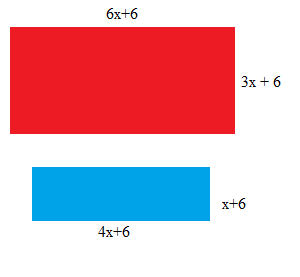
\includegraphics[width=2.04167in,height=1.8873in]{./imgSAEB_8_MAT/media/image5.png}

Deixar o espaço de 4 linhas para resposta.

Resposta:

Considerando a formula da área de um retângulo é l\textsuperscript{.} l
temos que

Terreno vermelho:

(6x+6) . (3x+6)=

18x²+18x+18x+36=

18x²+36x +36

Terreno azul:

(4x+6) . (x+6)=

4x²+24x+6x+36=

4x²+30x+36=

Somando os dois terrenos temos que

18x²+36x +36+4x²+30x+36=

Área total dos dois terrenos 22x²+66x+72

10) Efetue os monômios descritos abaixo:

a) 6x\textsuperscript{4}+ 12x\textsuperscript{6}

b)10xy-xy

c)(6x³) . (2x²)

d) (14x\textsuperscript{10)}: (2x²)

e) (2x³)³

f) (-4xy²) ³

g) (\frac{30x}{6x}) para x diferente de 0

h) 6x² - 8x²

i)((\frac{4}{5}x))\textsuperscript{-1}

j)9x² + 6x²

k) 7x² + 4x

l) (8r) . (6s)

m)(16x²) :4

n) 8x + 6x + 4x

o) (-4xy²)³

Em cada item acima deixar o espaço de 2 linhas para resposta.

Respostas:

Utilizando as propriedades algébricas e as propriedades de potenciação
temos que:

a) 6x\textsuperscript{4}+ 12x\textsuperscript{6}=18x\textsuperscript{10}

b)10xy-xy= 9xy

c)(6x³) . (2x²)=12x\textsuperscript{5}

d) (14x\textsuperscript{10)}: (2x²)=7x\textsuperscript{8}

e) (2x³)³= 2x\textsuperscript{9}

f) (-4xy²) ³= -4xy\textsuperscript{6}

g) (\frac{30x}{6x}) para x diferente de 0 = 5x

h) 6x² - 8x² = -2x²

i)((\frac{4}{5}x))\textsuperscript{-1}=+ (\frac{5}{4})

j)9x² + 6x²=15x²

k) 7x² + 4x²=11x²

l) (8r) . (6s)= 48rs

m)(16x²) :4= 4x²

n) 8x + 6x + 4x= 18x

o) (-2xy²)\textsuperscript{4}=
16x\textsuperscript{4}y\textsuperscript{8}

\colorsec{Treino}

1) Elza resolveu comprar uma piscina com as medidas abaixo:

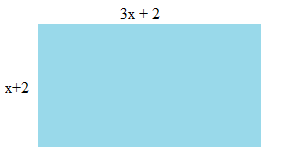
\includegraphics[width=2.9625in,height=1.67014in]{./imgSAEB_8_MAT/media/image6.png}

Qual a equação que representa a medida da área em m² dessa piscina?

a) 3x² +8x +4

b) 8x + 8

c) 4x + 4

d) 3x + 1

Resposta: A

BNCC: EF08MA10

Habilidade Saeb:

\begin{itemize}
\tightlist
\item
  Resolver problemas que envolvam cálculo do valor numérico de
  expressões algébricas.
\end{itemize}

A:Correta pois

Considerando a medida dos lados temos que:

3x+2^{.} x+2=

(3x+2)^{.} (x+2)=

Utilizando distributiva

3x² +6x +2x + 4

3x² +8x +4

B: incorreta, o aluno poderia confundir o enunciado e colocar o
resultado do perímetro ao invés da área chegando a este valor.

C: incorreta, o aluno poderia realizar uma soma ao invés de uma
multiplicação chegando a esse valor.

D: incorreta, o aluno poderia chegar a esse valor realizando uma divisão
ao invés de uma multiplicação.

2) Considerando que a²+ b² = 34 e ab= 15, qual o valor de
(\frac{(a + b)²}{8}) ?

a)2,266666666

b)19

c)8

d)9,25

Resposta: C

BNCC: EF08MA10

Habilidade Saeb

\begin{itemize}
\tightlist
\item
  Resolver problemas que envolvam cálculo do valor numérico de
  expressões algébricas.
\end{itemize}

A: incorreta o aluno chegaria a essa conclusão apenas dividindo um termo
pelo outro.

B: incorreta o aluno chegaria a essa conclusão realizando apenas a
subtração de um termo pelo outro.

C: Correta pois

(\frac{(a + b)²}{8}\ )= (\frac{a^{2} + 2ab + b²}{8})

Fazendo a substituição de a²+ b² = 34 e ab= 15 temos que:

(\frac{34 + (2.15)}{8} =) (\frac{34 + 30}{8}) = (\frac{64}{8}) = 8

D: incorreta pois ao realizar a soma ao invés da multiplicação no ultimo
termo

3) Ao comprar uma bola de futebol, Joaquim resolver fazer experimentos
com um disco de vinil, onde descobriu que o diâmetro do disco é igual a
(x² - 3), descobrindo o diâmetro Joaquim percebeu que era possível saber
o perímetro e a área do disco, ao realizar os cálculos quais valores
Joaquim descobriu?

Considere (\pi) = 3

a) Área = 3x\textsuperscript{4} - 18x² - 27 Perímetro= 6x² - 18

b) Área = 3x\textsuperscript{4} - 18x² + 27 Perímetro= 6x² + 18

c) Área = 3x\textsuperscript{4} + 18x² + 27 Perímetro= 6x² - 18

d) Área = 3x\textsuperscript{4} - 18x² + 27 Perímetro= 6x² - 18

Resposta: D

BNCC: EF08MA10

Habilidade Saeb:

\begin{itemize}
\tightlist
\item
  Resolver problemas que envolvam cálculo do valor numérico de
  expressões algébricas.
\end{itemize}

A: incorreta, o aluno ao errar o jogo de sinal no cálculo da área o
valor ficará desta forma.

B: incorreta, o aluno ao errar o jogo de sinal no cálculo do perímetro o
valor ficará desta forma.

C: incorreta, o aluno ao errar o jogo de sinal no cálculo da área o
valor ficará desta forma.

D: correta pois:

Para o cálculo da área

\[A = \pi r^{2}\]

Logo

A= 3 . (x²-3) ²

A= 3 . (x\textsuperscript{4} -- 6x² + 9)

A= 3x\textsuperscript{4}- 18x² + 27

Perímetro

% REVER
% P= 2(\text{\ π\ .\ r})

P= 2 . 3.(x²-3)

P= 2. (3x² - 9)

P= 6x² - 18

Logo resposta correta alternativa d.

\section{Módulo 7}

BNCC: EF08MA09

Habilidades Saeb:

\begin{itemize}
\item
  Inferir uma equação polinomial de 2º grau que modela um problema.
\item
  Resolver uma equação polinomial de 2º grau.
\item
  Resolver problemas que possam ser representados por equações
  polinomiais de 2º grau.
\end{itemize}

Equação polinomial de 2º grau

É considerada equação de polinomial de 2° grau, equações na forma ax² +
b = 0

Por exemplo:

Qual é a solução da equação x² - 9 = 0, no conjunto R

Temos que:

X² - 9 = 0

X²= 9

X = (\sqrt{9})

X = ± 3

Conjunto solução é \{- 3, 3\}

Resolução da equação 16x² - 1 = 0

16x² = 1

X = ( \pm \sqrt{\frac{1}{16}})

X = ( \pm \frac{1}{4})

Logo o conjunto solução é (+ \frac{1}{4}) e (- \ \frac{1}{4})

\colorsec{Atividades}

1) Determine a solução da equação x² + 4 = 0 no conjunto R

Deixar o espaço de 2 linhas para resposta.

Resposta: x² + 4 = 0

X² = - 4

X= (\sqrt{- 4})

Como (\sqrt{- 4}) não existe no conjunto R não temos valores reais
para x. Logo, a equação não tem raízes reais. Assim, S = \sout{0}

2) Resolva, no conjunto R, a equação (2y + 1) ² = 8 + 2(2y + 1).

Deixar o espaço de 6 linhas para resposta.

(2y + 1)(2y + 1) = 8 + 2(2y + 1)

4y² + 2y + 2y + 1 = 8 + 4y + 2

4y² + 4y + 1 = 10 + 4y

4y² + 4y - 4y + 1 - 10 = 0

4y² - 9 = 0

Y= ± (\sqrt{\frac{9}{4}})

Y= ± (\frac{3}{2})

Logo os números + (\frac{3}{2}) e (\frac{3}{2}) são as raízes da
equação.

3) Determine o conjunto solução de cada uma das seguintes equações do 2°
grau, no conjunto R

a) x² - 1 = 0

b) x² - 16 = 0

c) x² - 64 = 0

d) 9x² = 25

Em cada item acima deixar o espaço de 4 linhas para resposta.

Respostas:

a) \{ -1,1\}

b) \{ -4 , 4\}

c) \{-8, 8\}

d) \{(- \frac{5}{3}) ,(\frac{5}{3}) \}

4) Identifique a, b e c nas funções quadráticas abaixo:

a) x² -- 5x + 6 = 0

b) -2x² + 8x -- 8 = 0

c) x² = 4

d) x² - x = - (x + 15)

Deixar o espaço de 4 linhas para resposta.

Respostas:

a)

A= 1

B= -5

C= 6

b)

A = -2

B = 8

C = -8

c)

A = 1

B = 0

C = 4

d)

A=1

B= 0

C= 15

5) Joana é mãe de 3 crianças, a idade de seu filho mais novo é
representado pela equação x² -- 100 = 0, qual a idade do filho mais novo
de Joana? Deixar o espaço de 4 linhas para resposta.

Resposta: Realizando a equação temos que:

X² - 100 = 0

X² = 100

X = (\sqrt{100})

X= ±10

Como a idade não pode ser representada com números negativos temos que a
idade do filho mais novo de Joana é 10 Anos.

6) Marcos é dono de uma madeireira que vende blocos de madeira de 2
tamanhos diferentes, os tamanhos são definidos em metros, pelas raízes
da equação x² -- 5x + 4 = 0, quais são os tamanhos de madeira
disponíveis na madeireira de marcos? Deixar o espaço de 4 linhas para
resposta.

Resposta:

Temos que: x² -- 5x + 4 = 0

A= 1

B= - 5

C= 4

\[\frac{- ( - 5) \pm \sqrt{{- 5}^{2} - 4.\ 1.4}}{2.1}\]

\[\frac{5 \pm \sqrt{25 - 16}}{2}\]

\[\frac{5 \pm \sqrt{9}}{2}\]

\[\frac{5 \pm 3}{2}\]

X\textsubscript{1} = (\frac{5 + 3}{2})= (\frac{8}{2}) = 4

X\textsubscript{2} = (\frac{5 - 3}{2})= (\frac{2}{2})=1

Logo os tamanhos disponíveis de madeira são 1 metro e 4 metros.

7) Evandro é corredor, certo dia resolveu correr uma maratona com seu
amigo José, como Evandro é mais experiente que José largou na frente e
abriu certa vantagem, a distância de Evandro e José em km é definida
pela equação X² -- 4x + 4 = 0, sendo assim quantos km Evandro está na
frente de José? Deixar o espaço de 4 linhas para resposta.

Resposta:

x² -- 4x + 4 = 0

A=1

B= -4

C= 4

\[\frac{- ( - 4) \pm \sqrt{{( - 4)}^{2} - 4\ .\ 1.\ 4}}{2\ .\ 1}\]

\[\frac{4 \pm \sqrt{16 - 16}}{2}\]

(\frac{4}{2})=2 km

8) Raiane vai para o trabalho todos os dias a pé, a distância de sua
casa para o seu tralho em km é a soma das raízes da equação 2𝑥² − 6𝑥 − 8
= 0, quantos km Raiane anda por dia para ir ao trabalho? Deixar o espaço
de 4 linhas para resposta.

Resposta:

2𝑥² − 6𝑥 − 8 = 0

A=2

B= -6

C= -8

\[\frac{- ( - 6) \pm \sqrt{{( - 6)}^{2} - 4.2.( - 8)}}{2.2}\]

\[\frac{6 \pm \sqrt{36 + 64}}{4}\]

\[\frac{6 \pm \sqrt{100}}{4}\]

\[\frac{6 \pm 10}{4}\]

X1= (\frac{6 + 10}{4}) = (\frac{16}{4}) = 4

X2= (\frac{6 - 10}{4}) = (\frac{- 4}{4}) = -1

Somando ambas as raízes temos que Raiane anda 3km por dia para ir ao
trabalho.

9) Divina tem 2 filhas com idades diferentes, as idades das filhas de
divina são as raízes da equação x² - 20x + 36 = 0, qual a idade das
filhas de divina? Deixar o espaço de 4 linhas para resposta.

Resposta:

x² - 20x + 36 = 0

A= 1

B= -20

C= 36

\[\frac{- ( - 20) \pm \sqrt{{( - 20)}^{2} - 4.1.36}}{2.1}\]

\[\frac{20 \pm \sqrt{400 - 4.1.36}}{2a}\]

\[\frac{20 \pm \sqrt{400 - 144}}{2}\]

\[\frac{20 \pm \sqrt{256}}{2}\]

\[\frac{20 \pm 16}{2}\]

X1 = (\frac{20 + 16}{2})= (\frac{36}{2} =) 18

X2 = (\frac{20 - 16}{2}) = (\frac{4}{2}) = 2

Logo as filhas de Divina tem 18 anos e 2 anos.

10) Mateus está procurando pagar uma dívida com o banco, ele sabe que o
valor que deve é a soma da raízes da equação X²+4x+3 = 0 multiplicado
por 1 000, sendo assim quantos reais Mateus deve ao banco? Deixar o
espaço de 4 linhas para resposta.

Resposta: Utilizando Bhaskhara temos:

X²+4x+3 = 0

A= 1

B= 4

C= 3

\[\frac{- 4 \pm \sqrt{4^{2} - 4.1.3}}{2.1}\]

\[\frac{- 4 \pm \sqrt{16 - 4.1.3}}{2.1}\]

\[\frac{- 4 \pm \sqrt{4}}{2}\]

X1= (\frac{- 4 + 4}{2}) = 0

X2 = (\frac{- 4 - 4}{2}) = -4

Multiplicando por 1 000, temos que -4 . 1000 = - 4000

Logo Mateus deve 4 000,00 R\$ ao banco.

\colorsec{Treino}

1) Clebinho é atacante de um famoso time de futebol, durante uma partida
o número de finalizações de Clebinho no gol foi a soma das raízes da
equação x²- 7x=0, quantas vezes Clebinho chutou no gol durante a
partida?

a) 0

b) 7

c) 49

d) 14

Resposta: B

BNCC: EF09MA09

Habilidade Saeb:

\begin{itemize}
\tightlist
\item
  Resolver problemas que possam ser representados por equações
  polinomiais de 2º grau.
\end{itemize}

a incorreta: o aluno pode chegar a essa conclusão considerando que o
enunciado pede apenas 1 valor das raízes da equação descrita e não a
soma das raízes, chegando a essa conclusão erroneamente.

B: Correta, pois:

Utilizando Bhaskhara temos:

x² - 7x=0

A= 1

B= - 7

C= 0

\[\frac{- ( - 7) \pm \sqrt{{( - 7)}^{2} - 4.1.0}}{2.1}\]

\[\frac{7 \pm \sqrt{49}}{2}\]

\[\frac{7 \pm 7}{2}\]

X1 = (\frac{7 + 7}{2}) = (\frac{14}{2}) = 7

X2 = (\frac{7 - 7}{2}) = 0

Logo realizando a soma de 7+0 = 7 obtemos que Clebinho chutou 7 vezes ao
gol.

C: incorreta: o aluno pode chegar a essa conclusão considerando que o
enunciado pede apenas o valor antes de se extrair das raízes da equação
descrita e não a soma das raízes, chegando a essa conclusão
erroneamente.

D: incorreta: o aluno pode chegar a essa conclusão esquecendo de dividir
o valor de uma das raízes por 2, assim chegaria a esse valor
erroneamente.

2) Daniel é piloto de corridas de alta velocidade, em uma certa corrida
Daniel ficou em 2° lugar, a distância em segundos do primeiro colocado
para Daniel, é a soma das raízes da equação 4x² + 9x=0, quanto tempo
depois do primeiro colocado Daniel Chegou?

a)0

b) 81

c) 9

d) 2,25

Resposta: D

BNCC: EF09MA09

Habilidade Saeb:

\begin{itemize}
\tightlist
\item
  Resolver problemas que possam ser representados por equações
  polinomiais de 2º grau.
\end{itemize}

A: incorreta: o aluno pode chegar a essa conclusão considerando que o
enunciado pede apenas 1 valor das raízes da equação descrita e não a
soma das raízes, chegando a essa conclusão erroneamente.

B :incorreta: o aluno pode chegar a essa conclusão considerando que o
enunciado pede apenas o valor antes de se extrair das raízes da equação
descrita e não a soma das raízes, chegando a essa conclusão
erroneamente.

C: incorreta: o aluno pode chegar a essa conclusão esquecendo de dividir
o valor de uma das raízes por 4, assim chegaria a esse valor
erroneamente.

D: correta pois:

Utilizando Bhaskhara temos:

4x² + 9x=0

A= 4

B= 9

C= 0

\[\frac{- 9 \pm \sqrt{9^{2} - 4.4.0}}{2.4}\]

\[\frac{- 9 \pm \sqrt{81}}{8}\]

\[\frac{- 9 \pm 9}{8}\]

X1 = (\frac{- 9 + 9}{8}) = 0

X2= (\frac{- 9 - 9}{8}) = (\frac{- 18}{8}) = - (\frac{9}{4}) =
-2,25 segundos

3) Antônio foi ao posto de gasolina abastecer seu carro, ao final do
abastecimento descobriu que a quantidade do tanque que foi preenchida
por gasolina é igual a soma das raízes da equação 6x² - 5x = 0, qual foi
esta parte preenchida

a) 25

b) 0

c) (\frac{5}{6})

d) 11

Resposta: C

BNCC: EF09MA09

Habilidade Saeb

\begin{itemize}
\tightlist
\item
  Resolver problemas que possam ser representados por equações
  polinomiais de 2º grau.
\end{itemize}

A: incorreta o aluno pode chegar a esse valor ao não realizar a
radiciação necessária e não completar a equação como é determinante para
chegar ao resultado.

B: incorreta: o aluno pode chegar a essa conclusão considerando que o
enunciado pede apenas 1 valor das raízes da equação descrita e não a
soma das raízes, chegando a essa conclusão erroneamente.

C: Correta pois:

Utilizando Bhaskhara temos:

6x² - 5x = 0

A=6

B= -5

C= 0

\[\frac{- ( - 5) \pm \sqrt{{( - 5)}^{2} - 4.6.0}}{2( - 5)}\]

\[\frac{5 \pm \sqrt{25}}{12}\]

\[\frac{5 \pm 5}{12}\]

X1 = (\frac{5 + 5}{12}) = (\frac{10}{12}) = (\frac{5}{6})

X2= (\frac{5 - 5}{12}) = 0

Logo temos que a parte preenchida do tanque foi de (\frac{5}{6}).

D: incorreta, o aluno chegaria a esse valor apenas somando os termos da
equação e não realizando a operação por completo.

\section{Módulo 8}

BNCC: EF08MA12 EF08MA13

Habilidade Saeb:

\begin{itemize}
\tightlist
\item
  Resolver problemas que envolvam variação de proporcionalidade direta
  ou inversa entre duas ou mais grandezas, inclusive escalas, divisões
  proporcionais e taxa de variação.
\end{itemize}

Razão e proporção

Sendo a e b dois números racionais, com b ≠ 0, denomina-se razão entre a
e b ou razão de a para b o quociente (\frac{a}{b}) ou a:b A razão
(\frac{a}{b}\ )ou a : b pode ser lida de uma das seguintes maneiras:
razão de a para b ou a está para b ou a para b

Em razão e proporção podemos trabalhar com Grandezas proporcionais ou
Grandezas não proporcionais

Escala

Uma das aplicações da ideia de razão entre duas grandezas encontra-se na
escala de redução e na escala de ampliação, conhecidas simplesmente como
escala.

Denomina-se escala de um desenho a razão entre o comprimento considerado
nele e o correspondente comprimento real, medidos com a mesma unidade.
Em geral, utilizamos as medidas em centímetro para determinar uma
escala.

Escala =
% REVER
% (\frac{\text{comprimento\ de\ um\ desenho}}{\text{comprimento\ real}})

Densidade de um corpo

Para calcular a densidade de um corpo, também se aplica a ideia de razão
entre duas grandezas. Assim, a densidade de um corpo é dada pela razão
entre a massa e o volume desse corpo.

% REVER
%\[densidade = \ \frac{\text{massa\ do\ corpo}}{\text{volume\ do\ corpo}}\]

Questões

1) . Um prêmio de loteria, no valor de R\$ 2 700 000, 00 será dividido
igualmente pelo total de acertadores.

a) Quanto cada acertador receberá, se o prêmio for dividido entre 3
ganhadores?

b) E se fossem 8 ganhadores?

c) Conforme o número de acertadores aumenta, o que acontece com o valor
do prêmio?

Em cada item acima Deixar o espaço de 2 linhas para resposta.

Respostas:

a) ao dividir o valor do prêmio proporcionalmente entre 3 ganhadores
temos que

2 700 000 : 3 = 900 000 para cada um.

b) ao dividir o valor do prêmio proporcionalmente entre 8 ganhadores
temos que

2 700 000 : 8 = 337 500 para cada um.

c) Quando o número de acertadores aumenta o valor do prêmio diminui.

2) A distância entre a Terra e o Sol é de, aproximadamente, 150 000 000
km; A luz do Sol, para atingir a Terra, leva em torno de 500 segundos.

Responda:

a) Qual é a velocidade da luz no vácuo?

b) Quantos minutos a luz do Sol leva para chegar à Terra?

Deixar o espaço de 4 linhas para resposta.

a) Utilizando a razão 
% REVER
%(\frac{distância}{\text{tempo}}) temos que
(\frac{150\ 000\ 000}{500}) = 300 000 km/s

b) se 60 segundos = 1 minuto temos que 500 : 60 = 8 minutos e 20
segundos.

3) Um novo condomínio de casas está sendo construído e sua planta foi
representada, em uma folha de papel, com 5,5 cm de comprimento por 3,125
cm de largura. Sabendo que a escala utilizada foi 1 : 16 000, determine
as dimensões reais deste condomínio.

Deixar o espaço de 4 linhas para resposta.

Como a escala é de 1: 16 000 temos que:

Comprimento 5,5 . 16 0000= 88 000 cm

Largura 3,125 . 16 000 = 50 000 cm

Transformando em metros temos que

Comprimento= 880 m

Largura= 500 m

4) . Um bloco maciço de madeira tem 54 kg de massa e ocupa um volume de
3 m³. Qual a densidade desse bloco?

Deixar o espaço de 4 linhas para resposta.

Utilizando a razão da densidade que é (d = \frac{m}{v}) temos que

(d = \frac{54}{3})

d= 18 kg/m³

5) . Um fio de cobre utilizado na fiação de uma casa comum ocupa um
volume de 0,2 cm³. Sabendo que a massa do fio é de 4,3 g, determine a
densidade desse metal.

Deixar o espaço de 4 linhas para resposta.

Utilizando a razão da densidade que é (d = \frac{m}{v}) temos que:

(d = \frac{4,3}{0,2})

D= 21,5g/cm³

6) Um país situado no continente europeu, tem cerca de 135 000 km² de
área e uma população de 12 200 000 habitantes. Qual é a densidade
demográfica aproximada desse país?

Deixar o espaço de 4 linhas para resposta.

Utilizando a razão da densidade demográfica que é

(densidade\ demografica = \frac{número\ de\ pessoas\ }{dimensão\ do\ espaço\ em\ km²})
Temos que:

(densidade\ demografica = \frac{12\ 200\ 000}{135\ 000})

(densidade\ demografica =) 90,37 Habitantes/ km²

7) Cinco homens levam 20 dias para recapear um trecho de estrada. Esse
mesmo serviço seria realizado em quantos dias, se fossem 8 homens no
total?

Deixar o espaço de 4 linhas para resposta.

Utilizando a Regra de 3 simples temos que:

5 homens
-\/-\/-\/-\/-\/-\/-\/-\/-\/-\/-\/-\/-\/-\/-\/-\/-\/-\/-\/-\/-\/-\/-\/-20
dias

8 homens
-\/-\/-\/-\/-\/-\/-\/-\/-\/-\/-\/-\/-\/-\/-\/-\/-\/-\/-\/-\/-\/-\/-\/-\/-
x

5 . 20 = 8 . x

100 = 8x

X= 12,5

8) Uma Padaria produz 260 pães franceses a cada 50 min. Em uma jornada
de 12 h, quantos pães são produzidos?

Deixar o espaço de 4 linhas para resposta.

Utilizando a Regra de 3 simples temos que:

260 pães
-\/-\/-\/-\/-\/-\/-\/-\/-\/-\/-\/-\/-\/-\/-\/-\/-\/-\/-\/-\/-\/-\/-\/-50
minutos

X
-\/-\/-\/-\/-\/-\/-\/-\/-\/-\/-\/-\/-\/-\/-\/-\/-\/-\/-\/-\/-\/-\/-\/-\/-\/-\/-\/-\/-\/-\/-\/-\/-\/-\/-
720 minutos

187 200 = x . 50

X= 3744 pães são produzidos

9) Um livro tem 180 páginas, e cada página tem 46 linhas. Um editor
resolveu colocar apenas 30 linhas em cada página. Qual será a nova
quantidade de páginas do livro?

Deixar o espaço de 4 linhas para resposta.

Utilizando a Regra de 3 simples temos que:

180 páginas
-\/-\/-\/-\/-\/-\/-\/-\/-\/-\/-\/-\/-\/-\/-\/-\/-\/-\/-\/-\/-\/-\/-\/-46
linhas

X
-\/-\/-\/-\/-\/-\/-\/-\/-\/-\/-\/-\/-\/-\/-\/-\/-\/-\/-\/-\/-\/-\/-\/-\/-\/-\/-\/-\/-\/-\/-\/-\/-\/-\/-
30 linhas

180 . 46 = 30 . x

8280 = 30x

X= 276

10) Converta as velocidades dadas em m/s para km/h:

a) 20 m/s

b) 100 m/s

c) 55 m/s

d) 67 m/s

e) 90 m /s

f) 25 m/s

g) 30 m/s

h) 40 m/s

em cada item acima deixar o espaço de 2 linhas para resposta.

Respostas:

Para realizar a conversão de m/s para km/h devemos fazer a multiplicação
por 3,6

a) 20 m/s . 3,6= 72 km/h

b) 100 m/s . 3,6= 360km/h

c) 55 m/s . 3,6= 198 km/h

d) 67 m/s . 3,6= 241,2 km/h

e) 90 m /s . 3,6= 324 km/h

f) 25 m/s . 3,6= 90 km/h

g) 30 m/s .3,6= 108 km/h

h) 40 m/s . 3,6= 144km/h

\colorsec{Treino}

1) Dona Estela está preparando a Ceia de Natal para sua família e
comprou um peru de 4,2 kg para servir, ao pesquisar sobre o tempo de
cozimento de um peru descobriu que o tempo depende de sua massa em
quilogramas. Ao ler que um peru de 3,5 kg leva 2h15min para assar,
quanto tempo o peru que Dona estela comprou deve ficar no forno?

a) 2 horas e 42 minutos

b) 1 Horas e 52 minutos

c) 2 horas e 58 minutos

d) 567 minutos

Resposta: A

BNCC: EF08MA12 EF08MA13

Habilidade Saeb:

\begin{itemize}
\tightlist
\item
  Resolver problemas que envolvam variação de proporcionalidade direta
  ou inversa entre duas ou mais grandezas, inclusive escalas, divisões
  proporcionais e taxa de variação.
\end{itemize}

A: correta, pois:

Utilizando a Regra de 3 simples temos que:

3,5 kg
-\/-\/-\/-\/-\/-\/-\/-\/-\/-\/-\/-\/-\/-\/-\/-\/-\/-\/-\/-\/-\/-\/-\/-
135 minutos

4,2
kg-\/-\/-\/-\/-\/-\/-\/-\/-\/-\/-\/-\/-\/-\/-\/-\/-\/-\/-\/-\/-\/-\/-\/-x
minutos

3,5 . x = 567

X= 162 minutos ou 2 horas e 42 minutos

B: incorreta, o aluno poderia chegar a esse valor realizando a
multiplicação reta na regra de 3 e não a multiplicação cruzada.

C: incorreta, esse seria o valor caso o aluno não convertesse horas em
minutos como forma de solução, chegando a um valor equivocado.

D: incorreta, o aluno chegaria a esse resultado caso não realizasse a
última operação necessária, que é a divisão.

2) 5 rosquinhas de coco possuem 64 calorias. Dirce consome diariamente 3
rosquinhas em seu café da manhã. Quantas calorias procedentes das
rosquinhas Dirce consome por dia?

a) 106,6 calorias

b) 38,4 calorias

c) 960 calorias

d) 192 calorias

Resposta: B

BNCC: EF08MA12 EF08MA13

Habilidade Saeb:

\begin{itemize}
\tightlist
\item
  Resolver problemas que envolvam variação de proporcionalidade direta
  ou inversa entre duas ou mais grandezas, inclusive escalas, divisões
  proporcionais e taxa de variação.
\end{itemize}

A: incorreta, o aluno chegaria nesse resultado multiplicando reto a
regra de três ao invés de multiplicar cruzado.

B: correta pois:

Utilizando a Regra de 3 simples temos que:

5 rosquinhas
-\/-\/-\/-\/-\/-\/-\/-\/-\/-\/-\/-\/-\/-\/-\/-\/-\/-\/-\/-\/-\/-\/-\/-64
calorias

3 rosquinhas
-\/-\/-\/-\/-\/-\/-\/-\/-\/-\/-\/-\/-\/-\/-\/-\/-\/-\/-\/-\/-\/-\/- x
calorias

5x = 64 . 3

5x = 192

X= 38,4

C: incorreta, o aluno chegaria a esse valor caso no final da expressão
ao invés de realizar uma divisão, realizar uma multiplicação.

D: incorreta, o auno chegaria a essa conclusão considerando que cada
rosquinha possuísse 64 calorias, interpretando errado o enunciado.

3) Leandro tem um cachorro da raça fila brasileiro que pesa 27 kg. Para
tratar uma infecção nas vias urinárias, o veterinário receitou um
antibiótico cuja dosagem é de 9 ml a cada 10 kg de peso corporal.
Quantos ml de antibiótico Leandro dará a seu cachorro?

a) 3,3333.\ldots. ml

b) 24,3ml

c) 2430 ml

d) 2,43 ml

Resposta: B

\section{Módulo 9}

BNCC: EF08MA12 EF08MA13

Habilidade Saeb:

\begin{itemize}
\tightlist
\item
  Resolver problemas que envolvam variação de proporcionalidade direta
  ou inversa entre duas ou mais grandezas, inclusive escalas, divisões
  proporcionais e taxa de variação.
\end{itemize}

A: incorreta, o aluno chegaria a esse resultado realizando uma
multiplicação reta ao invés de uma multiplicação cruzada, na regra de 3
simples.

B: Correta: pois

Utilizando a Regra de 3 simples temos que:

10 kg
-\/-\/-\/-\/-\/-\/-\/-\/-\/-\/-\/-\/-\/-\/-\/-\/-\/-\/-\/-\/-\/-\/-\/-9ml

27
kg-\/-\/-\/-\/-\/-\/-\/-\/-\/-\/-\/-\/-\/-\/-\/-\/-\/-\/-\/-\/-\/-\/-\/-x
ml

10.x= 9 . 27

10x= 243

X= 24,3 ml

C: incorreta, o aluno chegaria a essa conclusão ao final da expressão ao
invés de realizar uma divisão realizar uma multiplicação.

D: incorreta, o aluno chegaria a essa conclusão deslocando a virgula uma
casa para esquerda durante o cálculo final.

\section{Módulo 10}

BNCC: EF08MA18

Habilidades Saeb:

Identificar, no plano cartesiano, figuras obtidas por uma ou mais
transformações geométricas (reflexão, translação, rotação).

\begin{itemize}
\item
  Relacionar o número de vértices, faces ou arestas de prismas ou
  pirâmides, em função do seu polígono da base.
\item
  Relacionar objetos tridimensionais às suas planificações ou vistas.
\item
  Classificar polígonos em regulares e não regulares. - Reconhecer
  polígonos semelhantes ou as relações existentes entre ângulos e lados
  correspondentes nesses tipos de polígonos.
\item
  Reconhecer circunferência/círculo como lugares geométricos, seus
  elementos (centro, raio, diâmetro, corda, arco, ângulo central, ângulo
  inscrito).
\item
  Construir/desenhar figuras geométricas planas ou espaciais que
  satisfaçam condições dadas.
\end{itemize}

Polígono é uma figura plana formada por uma linha fechada simples,
composta apenas de segmentos de reta, reunida com a sua região interna.

Podemos Classificar os polígonos em convexos e não convexos

Podemos destacar os seguintes elementos de um polígono: vértices, lados,
ângulos internos e externos e diagonais

Utilizando a Fórmula (d = \ \frac{n(n - 3)}{2}) podemos determinar o
número de diagonais de um polígono

Utilizando a fórmula S\textsubscript{i} = (n-2) . 180° , podemos
calcular a soma dos ângulos internos de um polígono.

\colorsec{Atividades}

1) Complete a Tabela com o nome dos polígonos segundo o número de lados

\begin{longtable}[]{@{}ll@{}}
\toprule
Número de lados & Nome do Polígono\tabularnewline
\midrule
\endhead
3 & Triângulo\tabularnewline
4 & ~\tabularnewline
5 & ~\tabularnewline
6 & ~\tabularnewline
7 & ~\tabularnewline
8 & ~\tabularnewline
9 & ~\tabularnewline
10 & ~\tabularnewline
11 & ~\tabularnewline
12 & ~\tabularnewline
15 & ~\tabularnewline
20 & ~\tabularnewline
\bottomrule
\end{longtable}

Inserir uma tabela similar a essa, contendo os mesmo valores, podendo
ser modificada o estilo e as cores .

Resposta:

\begin{longtable}[]{@{}ll@{}}
\toprule
Número de lados & Nome do Polígono\tabularnewline
\midrule
\endhead
3 & Triângulo\tabularnewline
4 & Quadrilátero\tabularnewline
5 & Pentágono\tabularnewline
6 & Hexágono\tabularnewline
7 & Heptágono\tabularnewline
8 & Octógono\tabularnewline
9 & Eneágono\tabularnewline
10 & Decágono\tabularnewline
11 & Eneágono\tabularnewline
12 & Dodecágono\tabularnewline
15 & Pentadecágono\tabularnewline
20 & Icoságono\tabularnewline
\bottomrule
\end{longtable}

2) Determine quais das figuras abaixo são polígonos

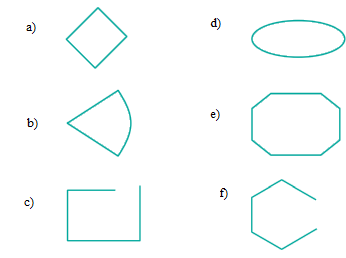
\includegraphics[width=1.7in,height=1.26763in]{./imgSAEB_8_MAT/media/image7.png}

Inserir figuras similares a estas contendo o mesmo formato

Resposta: As figuras que são polígonos são somente alternativa A e E

3) Classifique os polígonos abaixo em convexos e não convexos

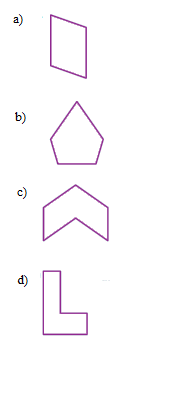
\includegraphics[width=1.16236in,height=2.36667in]{./imgSAEB_8_MAT/media/image8.png}

Inserir figuras similares a estas contendo o mesmo formato.

Respostas:

a) convexo

b) convexo

c) não convexo

d) não convexo

4) Utilizando a Fórmula (d = \ \frac{n(n - 3)}{2}) para determinar o
número de diagonais de um polígonos calcule o número de diagonais de um
polígono de

a) 5 lados

b) 9 lados

c) 10 lados

d) 15 lados

e) 20 lados

em cada item cima deixar o espaço de 4 linhas para resposta.

Repostas:

% REVER
% Utilizando (d = \ \frac{n(n - 3)}{2}\text{\ \ })temos que

a) (d = \ \frac{5(5 - 3)}{2}) = (\frac{25 - 15}{2}) =
(\frac{10}{2}) = 5 diagonais

b) (d = \ \frac{9(9 - 3)}{2}) = (\frac{81 - 27}{2} = \frac{54}{2})=
27 diagonais

c) (d = \ \frac{10(10 - 3)}{2}) =
(\frac{100 - 30}{2} = \frac{70}{2} =) 35 diagonais

d) (d = \ \frac{15(15 - 3)}{2}) = (\frac{225 - 45}{2})=
(\frac{180}{2})= 90 diagonais

e) (d = \ \frac{20(20 - 3)}{2})=
(\frac{400 - 60}{2} = \frac{340}{2})= 170 diagonais

5) Utilizando a fórmula S\textsubscript{i} = (n-2) . 180°, calcule a
soma dos ângulos internos dos polígonos abaixo

a) Quadrilátero

b) Pentágono

c) Eneágono

d) Icoságono

e) Dodecagono

em cada item acima deixar o espaço de 4 linhas para resposta.

Respostas:

Utilizando a fórmula S\textsubscript{i} = (n-2) . 180° temos que

a) Quadrilátero

S\textsubscript{i} = (4-2) . 180°

S\textsubscript{i=} 2 . 180 °

S\textsubscript{i}= 360°

b) Pentágono

S\textsubscript{i} = (5-2) . 180°

S\textsubscript{i}= 3 . 180

S\textsubscript{i}= 540

c) Eneágono

S\textsubscript{i} = (9-2) . 180°

S\textsubscript{i} = 7 . 180°

S\textsubscript{i} = 1260°

d) Icoságono

S\textsubscript{i} = (20-2) . 180°

S\textsubscript{i} = 18 . 180°

S\textsubscript{i} = 3240°

e) Dodecagono

S\textsubscript{i} = (12-2) . 180°

S\textsubscript{i} = 10 . 180

S\textsubscript{i} = 1800°

6) Utilizando a fórmula S\textsubscript{i} = (n-2) . 180°, calcule o
número de lados dos polígonos cuja soma dos ângulos internos são:

a) 1080°

b) 1980°

c) 2340°

d) 1800°

em cada item acima deixar o espaço de 4 linhas para resposta.

Respostas:

a) 1080°

1080 = (n-2) . 180°

(\frac{1080}{180})= n- 2

6 = n-2

N = 8

b) 1980°

1980 = (n-2) . 180°

(\frac{1980}{180}) = n -- 2

11 = n -2

N= 13

c) 2340°

2340= (n-2) . 180°

(\frac{2340}{180}) = n -- 2

13= n -- 2

N= 15

d) 1800°

1800 = (n-2) . 180°

(\frac{1800}{180})= n -- 2

10 = n- 2

N= 12

7) Considere o paralelogramo a seguir. Nele, estão expressas as medidas
de dois ângulos opostos. Quais são as medidas dos quatro ângulos desse
paralelogramo?

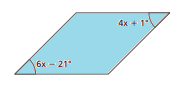
\includegraphics[width=1.82292in,height=0.95833in]{./imgSAEB_8_MAT/media/image9.png}

Inserir uma imagem similar a essa porém contendo o mesmo conteúdo
numérico

Deixar o espaço de 4 linhas para resposta.

Resposta:

Temos que

4x+1 = 6x -21

-2x = -22

X=11

Substituindo x = 11 nas duas equações temos que:

4.11+ 1 =45°

6.11-21= 45°

Como a soma dos ângulos internos de um paralelogramo é 360°

45° + 45° - 360° = 270°

270° : 2= 135°

Temos então que o paralelogramo possui 2 ângulos de 45° e 2 ângulos de
135°

8) Calcule o valor de x e y na figura indicada.

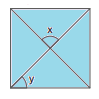
\includegraphics[width=1.03125in,height=1.03125in]{./imgSAEB_8_MAT/media/image10.png}

Inserir uma imagem similar a essa porém contendo o mesmo conteúdo
numérico

Deixar o espaço de 4 linhas para resposta.

Resposta:

Relembrando que a soma dos ângulos internos de um triangulo é = 180 °

E que a soma dos ângulos internos de um paralelogramo é igual a 360°

Temos que y=45° e x = 90°

9) Determine a medida x no paralelogramo da figura a seguir:

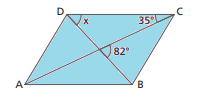
\includegraphics[width=2.05208in,height=1.09375in]{./imgSAEB_8_MAT/media/image11.png}

Inserir uma imagem similar a essa porém contendo o mesmo conteúdo
numérico

Deixar o espaço de 4 linhas para resposta.

Resposta:

Por método de observação temos que Ângulo no ponto B é:

82°+ 35° -- 180° =63°

Formando um triangulo BCD temos que

70° + 63° -- 180° = 47°

10) Analise a circunferência de centro A representada a seguir e
classifique em raio, diâmetro ou corda o segmento de reta:


\includegraphics[width=2.98681in,height=2.57292in]{./imgSAEB_8_MAT/media/image12.png}

Inserir uma imagem similar a essa porém contendo o mesmo conteúdo.

a) GA

b) DC

c) EF

d) GH

e) AB

f) DA

g) HI

h) AC

i) AH

Em cada item acima deixar o espaço de 1 linha para resposta.

Respostas:

a) raio

b) diâmetro; corda

c) corda

d) diâmetro; corda

e) raio

f) raio

g) corda

h) raio

i) raio

\colorsec{Treino}

1) Alfredo desenhou, em uma madeira, um eneágono regular cujo perímetro
era de 117 cm

Qual é a medida de cada lado dessa figura?

a) 13 cm

b) 11,7 cm

c) 16,71 cm

d) 23,4 cm

Resposta: A

BNCC: EF08MA18

Habilidade Saeb- Construir/desenhar figuras geométricas planas ou
espaciais que satisfaçam condições dadas.

A: Correta, pois

117 : 9 = 13 cm de lado tem essa figura.

B: incorreta, o aluno poderia chegar a essa conclusão caso considerasse
que o eneágono regular possui 10 lados e não 9.

c: incorreta, o aluno poderia chegar a essa conclusão caso considerasse
que o eneágono regular possui 7 lados e não 9.

D: incorreta, o aluno poderia chegar a essa conclusão caso considerasse
que o eneágono regular possui 5 lados e não 9.

2) O~centro do campo~de futebol é marcado com um ponto no~centro~da
linha de meio de~campo~(marca~central), ao redor se traça um~círculo~com
raio de 9,15 metros, com essas informações qual a área do círculo
central de um campo de futebol aproximadamente?

Considere (\pi = 3)

a) 54,1 m²

b) 27,41 m²

c) 251 m²

d) 27,66 m²

Resposta: C

BNCC: EF08MA18

Habilidade Saeb

\begin{itemize}
\tightlist
\item
  Reconhecer circunferência/círculo como lugares geométricos, seus
  elementos (centro, raio, diâmetro, corda, arco, ângulo central, ângulo
  inscrito).
\end{itemize}

A: incorreta, o aluno chegaria a esse valor caso confundisse a formula
da área do círculo com a formula do perímetro do círculo.

B: incorreta o aluno chegaria a essa conclusão, caso esquecesse do termo
quadrático da expressão.

C: Correta

pois:

\[A = \pi r^{2}\]

A = 3 . 9,15²

A= 3. 83,7225

A= 251 m²

D: incorreta, o aluno chegaria a esse resultado caso dividisse a
expressão no final da formula ao invés de multiplicar.

3) Iolanda faz peças com tecidos. Uma das peças mais vendidas por ela é
um porta joias com formato de um hexágono regular de 5 cm de lado, em
que toda borda é revestida com uma fita. Quantos centímetros de fita, no
mínimo, Iolanda precisa para confeccionar 20 porta joias desses?

a) 6 metros

b) 600 metros

c) 5 metros

d) 4 metros

Resposta: A

BNCC: EF08MA18

Habilidade Saeb:

\begin{itemize}
\tightlist
\item
  Relacionar o número de vértices, faces ou arestas de prismas ou
  pirâmides, em função do seu polígono da base.
\end{itemize}

A: Correta

Hexágono regular = 6 lados

\num{6} 5 = 30 cm por porta joias

20 . 30 cm = 600 cm de fita ou 6 metros de fita

B: incorreta, o aluno pode chegar a esse valor confundindo cm com
metros.

C: incorreta, o aluno pode chegar a esse valor considerando que um
hexágono regular contenha 5 lados

D: incorreta, o aluno pode chegar a esse valor considerando que um
hexágono regular contenha 4 lados.

\section{Módulo 11}

BNCC: EF08MA14

Habilidades Saeb:

\begin{itemize}
\item
  Identificar propriedades e relações existentes entre os elementos de
  um triângulo (condição de existência, relações de ordem entre as
  medidas dos lados e as medidas dos ângulos internos, soma dos ângulos
  internos, determinação da medida de um ângulo interno ou externo).
\item
  Classificar triângulos ou quadriláteros em relação aos lados ou aos
  ângulos internos.
\item
  Identificar retas ou segmentos de retas concorrentes, paralelos ou
  perpendiculares.
\item
  Identificar relações entre ângulos formados por retas paralelas
  cortadas por uma transversal.
\item
  Resolver problemas que envolvam relações entre ângulos formados por
  retas paralelas cortadas por uma transversal, ângulos internos ou
  externos de polígonos ou cevianas (altura, bissetriz, mediana,
  mediatriz) de polígonos.
\item
  Resolver problemas que envolvam relações métricas do triângulo
  retângulo, incluindo o teorema de Pitágoras.
\item
  Resolver problemas que envolvam polígonos semelhantes.
\item
  Resolver problemas que envolvam aplicação das relações de
  proporcionalidade abrangendo retas paralelas cortadas por
  transversais.
\item
  Determinar o ponto médio de um segmento de reta ou a distância entre
  dois pontos quaisquer, dadas as coordenadas desses pontos no plano
  cartesiano.
\end{itemize}

Triângulos

Elementos de um triângulo

\begin{itemize}
\item
  Vértices
\item
  Lados
\item
  Ângulos internos
\item
  Ângulos externos
\end{itemize}

Classificação de triângulos

Classificamos os triângulos em relação às medidas de seus lados ou às
medidas de seus ângulos internos. Em relação às medidas dos lados, um
triângulo é classificado como:

\begin{itemize}
\item
  Equilátero: Quando os três lados têm medidas iguais.
\item
  Isósceles: Quando dois lados têm medidas iguais.
\item
  Escaleno: Quando os três lados têm medidas diferentes.
\end{itemize}

Em relação às medidas dos ângulos, um triângulo é classificado como:

\begin{itemize}
\item
  Acutângulo: Quando os três ângulos internos são agudos (menores que
  90º)
\item
  Retângulo: Quando um dos ângulos internos é reto (medida igual a 90º).
\item
  Obtusângulo: Quando um dos ângulos internos é obtuso (a medida é maior
  que 90º e menor que 180º).
\end{itemize}

Bissetriz de um triângulo

Bissetriz de um triângulo é o segmento de reta que une um vértice do
triângulo ao seu respectivo lado oposto, dividindo o ângulo desse
vértice em dois ângulos de mesma medida.

Mediatriz

Mediatriz de um lado de um triângulo é a reta perpendicular a esse lado
que passa pelo seu ponto médio

Todo triângulo possui três mediatrizes, que se encontram em um único
ponto denominado circuncentro.

Triângulos congruentes

Dois triângulos são congruentes quando têm os lados e os ângulos
correspondentes congruentes.

Questões:

1) Observe a figura abaixo

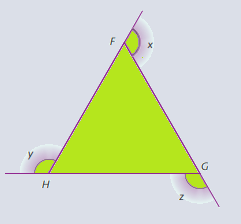
\includegraphics[width=1.88333in,height=1.75048in]{./imgSAEB_8_MAT/media/image13.png}

Inserir uma imagem similar a essa, podendo ser alterada as cores e o
estilo, mas que o conteúdo continue o mesmo.

a) os vértices do triângulo;

b) os lados do triângulo;

c) os ângulos internos do triângulo;

d) os ângulos externos do triângulo;

e) o lado oposto ao ângulo F

Deixar o espaço de 3 linhas para resposta em cada item acima

Respostas:

a) F, G e H

b) FH, FG E HG

c) F, G E H

d) x, y e z

e) HG

2) No triângulo representado a seguir, AD é bissetriz em relação a BÂC.
Determine o valor de x, em graus

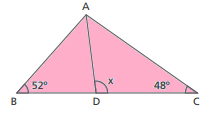
\includegraphics[width=2.20833in,height=1.1875in]{./imgSAEB_8_MAT/media/image14.png}

Inserir uma imagem similar a essa, podendo ser alterada as cores e o
estilo, mas que o conteúdo continue o mesmo.

Deixar o espaço de 3 linhas para resposta.

Resposta:

Considerando a soma dos ângulos internos temos que:

52+48 =100

Logo o ângulo BÂC= 80° e o valo de sua bissetriz 40°

Logo o ângulo x possui:

40+48=88

180-88= 92°

3) Em cada caso, analise se é possível construir um triângulo com lado
BC de 5 cm e com as medidas dos ângulos indicadas.

a) medida do ângulo (B)= 110° e medida do ângulo (C) = 50°

b) medida do ângulo (B) = 110° e medida do ângulo (C)= 70°

c) medida do ângulo (B) = 110° e medida do ângulo (C) = 90°

Deixar o espaço de 3 linhas para resposta em cada item acima.

Respostas:

Considerando que a soma dos ângulos internos do triangulo deve ser 180°
logo obtemos somando os ângulos das expressões que

a) é possível

b) não é possível

c) não é possível

4) Em cada triângulo representado a seguir, onde foram traçadas algumas
retas, identifique se o ponto O é circuncentro, incentro, baricentro ou
ortocentro.

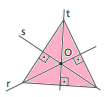
\includegraphics[width=1.14583in,height=1.01042in]{./imgSAEB_8_MAT/media/image15.png}a)

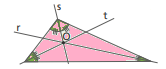
\includegraphics[width=1.72917in,height=0.71875in]{./imgSAEB_8_MAT/media/image16.png}b)


\includegraphics[width=1.84375in,height=1.125in]{./imgSAEB_8_MAT/media/image17.png}

c)

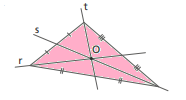
\includegraphics[width=1.9375in,height=1.04167in]{./imgSAEB_8_MAT/media/image18.png}

d)

Inserir imagens similares a essas, podendo ser alterada as cores e o
estilo, mas que o conteúdo continue o mesmo.

Deixar o espaço de 3 linhas para resposta.

Respostas:

A) Ortocentro

b) Incentro

c) Circuncentro

d) Baricentro

5) Em cada item, verifique se os triângulos são congruentes:

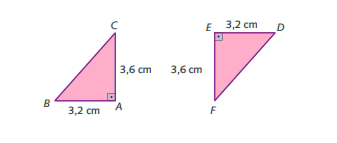
\includegraphics[width=3.51042in,height=1.48958in]{./imgSAEB_8_MAT/media/image19.png}a)

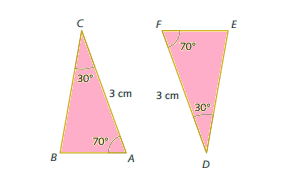
\includegraphics[width=3.16667in,height=2.03958in]{./imgSAEB_8_MAT/media/image20.png}b)

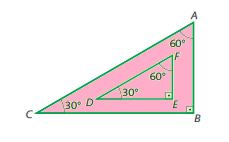
\includegraphics[width=2.38542in,height=1.47917in]{./imgSAEB_8_MAT/media/image21.png}c)

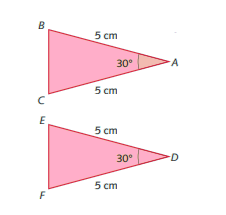
\includegraphics[width=2.35417in,height=2.23958in]{./imgSAEB_8_MAT/media/image22.png}d)


\includegraphics[width=2.73958in,height=1.54167in]{./imgSAEB_8_MAT/media/image23.png}

e)

Inserir imagens similares a essas, podendo ser alterada as cores e o
estilo, mas que o conteúdo continue o mesmo.

Deixar o espaço de 5 linhas para resposta.

Respostas:

a) São congruentes

b) São congruentes

c) Não são congruentes

d) são congruentes

e) são congruentes

6) Calcule, em grau, as medidas dos ângulos dos triângulos abaixo:

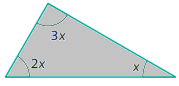
\includegraphics[width=1.86458in,height=0.89583in]{./imgSAEB_8_MAT/media/image24.png}a)

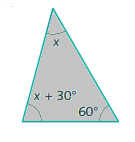
\includegraphics[width=1.40625in,height=1.47917in]{./imgSAEB_8_MAT/media/image25.png}

b)

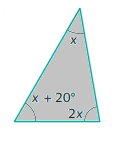
\includegraphics[width=1.30208in,height=1.5625in]{./imgSAEB_8_MAT/media/image26.png}

c)


\includegraphics[width=2.33333in,height=0.95833in]{./imgSAEB_8_MAT/media/image27.png}

d)

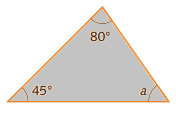
\includegraphics[width=1.83333in,height=1.1875in]{./imgSAEB_8_MAT/media/image28.png}

e)


\includegraphics[width=2in,height=1.30208in]{./imgSAEB_8_MAT/media/image29.png}

f)

Inserir imagens similares a essas, podendo ser alterada as cores e o
estilo, mas que o conteúdo continue o mesmo.

Em cada item acima deixar o espaço de 3 linhas para resposta.

Respostas: Considerando que a soma de todos os ângulos internos de um
triangulo deve ser 180° temos que

a)

3x+2x+x = 180

6x =180

X=30

Logos os respectivos ângulos são 30°,60° e 90°

b) x+ x+30 + 60 = 180

2x+90 =180

2x=90

X=45

Logo os ângulos são respectivamente 45°, 75° e 60 °

c)

x+x+20+2x =180

4x+20 =180

4x=160

X=40

Logo os ângulos são respectivamente 40°, 60° e 80°

d) a= 40°

e) a= 55°

f) a=108°

7) determine as medidas dos ângulos complementar e suplementar de cada
ângulo a seguir:

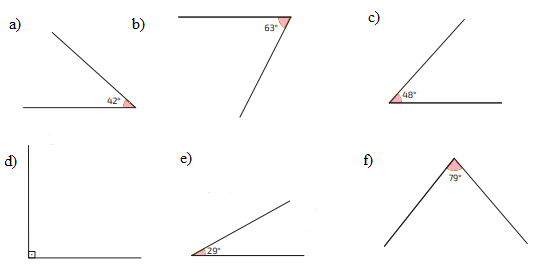
\includegraphics[width=4.81667in,height=2.48373in]{./imgSAEB_8_MAT/media/image30.png}

Inserir uma imagem similar a essa, podendo ser alterada as cores e o
estilo, mas que o conteúdo continue o mesmo.

Em cada item acima Deixar o espaço de 2 linhas para resposta.

Respostas:

a) 48° e 138°

b) 27° e 117°

c) 42° e 132°

d) 0° e 90°

e) 61° e 151°

F) 11° e 101°

8) Enzo ao folear um livro de engenharia de seu pai se deparou a
seguinte imagem:

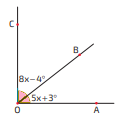
\includegraphics[width=1.47134in,height=1.42708in]{./imgSAEB_8_MAT/media/image31.png}

Inserir uma imagem similar a essa, podendo ser alterada as cores e o
estilo, mas que o conteúdo continue o mesmo.

Para encontrar o valor de x quais os passos que Enzo deve tomar?

Deixar o espaço de 3 linhas para resposta.

Resposta:

1° Observar que o ângulo destacado é igual a 90°

2° montar a equação da seguinte forma

8x-4+5x+3=90

13x -- 1 = 90

13x= 91

X= 7

9) Calcule as medidas do ângulos destacados abaixo, considerando que as
linhas em verde traçam a bissetriz de cada angulo

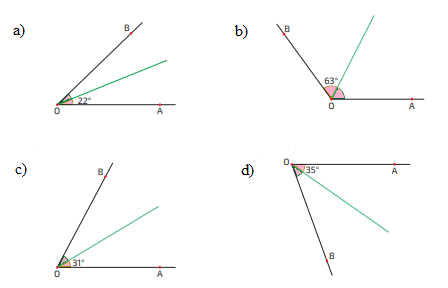
\includegraphics[width=4.66667in,height=3in]{./imgSAEB_8_MAT/media/image32.png}

Inserir imagens similares a essa, podendo ser alterada as cores e o
estilo, mas que o conteúdo continue o mesmo.

Deixar o espaço de 3 linhas para resposta.

Respostas

a) 44°

b) 126°

c) 62°

d) 70°

10) Calcule o valor de x nas figuras abaixo

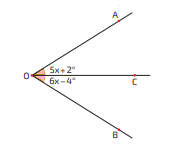
\includegraphics[width=1.91667in,height=1.6875in]{./imgSAEB_8_MAT/media/image33.png}

a)

Inserir uma imagem similar a essa, podendo ser alterada as cores e o
estilo, mas que o conteúdo continue o mesmo.

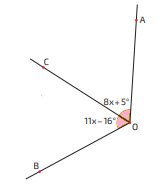
\includegraphics[width=1.80208in,height=2.02917in]{./imgSAEB_8_MAT/media/image34.png}b)

Inserir uma imagem similar a essa, podendo ser alterada as cores e o
estilo, mas que o conteúdo continue o mesmo.

Deixar o espaço de 3 linhas para resposta em cada item acima

Respostas:

a)

5x+2 = 6x -4

-x=-6

X=6

b)

11x-16=8x+5

3x= 21

X=7

\colorsec{Treino}

1) Denomina-se incentro o ponto comum

a) às alturas do triângulo;

b) às mediatrizes dos lados do triângulo;

c) às medianas do triângulo;

d) às bissetrizes do triângulo.

Resposta: D

BNCC: EF08MA14

Habilidade Saeb:

\begin{itemize}
\tightlist
\item
  Resolver problemas que envolvam relações entre ângulos formados por
  retas paralelas cortadas por uma transversal, ângulos internos ou
  externos de polígonos ou cevianas (altura, bissetriz, mediana,
  mediatriz) de polígonos.
\end{itemize}

A: incorreta, as relações no triangulo são ligeiramente semelhantes,
logo por definição o aluno deverá ter o conhecimento aflorado para
conseguir identificar o conceito de incentro, ao não compreender o
conceito completo logo esta alternativa pode ser uma resposta viável.

B: incorreta, as relações no triangulo são ligeiramente semelhantes,
logo por definição o aluno deverá ter o conhecimento aflorado para
conseguir identificar o conceito de incentro, ao não compreender o
conceito completo logo esta alternativa pode ser uma resposta viável.

C: incorreta, as relações no triangulo são ligeiramente semelhantes,
logo por definição o aluno deverá ter o conhecimento aflorado para
conseguir identificar o conceito de incentro, ao não compreender o
conceito completo logo esta alternativa pode ser uma resposta viável.

Resposta: Alternativa D as bissetrizes do triângulo.

2) O triângulo ABC é um triângulo retângulo em A e isósceles. O ponto O
é o seu circuncentro, ou seja, é o centro da circunferência circunscrita
ao triângulo. Se a altura relativa à hipotenusa BC mede 9,3~cm, qual é a
medida da hipotenusa?


\includegraphics[width=2.5625in,height=2.02083in]{./imgSAEB_8_MAT/media/image35.png}

Inserir uma imagem similar a essa, podendo ser alterada as cores e o
estilo, mas que o conteúdo continue o mesmo.

a) 9,3

b)18,2

c) 18,6

d) 18,8

Resposta: C

BNCC: EF08MA14

Habilidade Saeb

\begin{itemize}
\tightlist
\item
  Resolver problemas que envolvam relações entre ângulos formados por
  retas paralelas cortadas por uma transversal, ângulos internos ou
  externos de polígonos ou cevianas (altura, bissetriz, mediana,
  mediatriz) de polígonos.
\end{itemize}

A: Incorreta, este seria o valor relativo e não a medida final.

B: incorreta, ao errar o cálculo da multiplicação o valor chegará a
esse.

C: Correta pois:

Se a altura relativa à hipotenusa BC mede 9,3~cm, a medida da hipotenusa
será 18,6

D: Incorreta, o aluno chegara a esse conclusão ao errar o cálculo de
multiplicação dos termos destacados no enunciado.

3) Qual o perímetro de um triângulo com lados cujas medidas são 6 cm, 7
cm e 8 cm

a) 19 cm

b) 20 cm

c) 21 cm

d)22cm

Resposta: C

BNCC: EF08MA14

Habilidade Saeb

\begin{itemize}
\tightlist
\item
  Identificar propriedades e relações existentes entre os elementos de
  um triângulo (condição de existência, relações de ordem entre as
  medidas dos lados e as medidas dos ângulos internos, soma dos ângulos
  internos, determinação da medida de um ângulo interno ou externo)
\end{itemize}

A: incorreta, o aluno chegara a essa conclusão se durante o cálculo da
soma dos lados do triangulo o aluno equivocadamente chegar ao resultado
com 2 números a menos.

B: incorreta, o aluno chegara a essa conclusão se durante o cálculo da
soma dos lados do triangulo o aluno equivocadamente chegar ao resultado
com 1 número a menos.

Alternativa: C Correta.

Perímetro= soma dos lados

Logo 6 + 7 + 8 = 21cm

D: incorreta, o aluno chegara a essa conclusão se durante o cálculo da
soma dos lados do triangulo o aluno equivocadamente chegar ao resultado
com 1 número a mais.

\section{Módulo 12}

\begin{itemize}
\tightlist
\item
  Descrever ou esboçar deslocamento de pessoas e/ou de objetos em
  representações bidimensionais (mapas, croquis etc.), plantas de
  ambientes ou vistas, de acordo com condições dadas.
\end{itemize}

Mapas

Mapa é uma~\textbf{representação gráfica de um espaço real, em uma
superfície plana, como um papel, cartolina, madeira, pintura realiza em
diferentes materiais, um mapa pode representar espaços reais contendo
informações precisas e detalhadas sobre espaços do cotidiano.}

\textbf{Croquis}

\textbf{São representações feitas a mão de um espaço que pode ser real
ou não, como um vilarejo ilusório ou até mesmo uma descrição de um
espaço que só o autor do croqui reconhece.}

\textbf{Deslocamento}

\textbf{O deslocamento pode ser considero a distância percorrida por um
objeto ou alguém durante um período: que pode ser representado pela
formula:}

Distancia = Velocidade média X tempo

Questões

1) Paulo está pretendendo fazer uma longa viagem para visitar seus pais,
nos quais ele não os vê a muitos anos

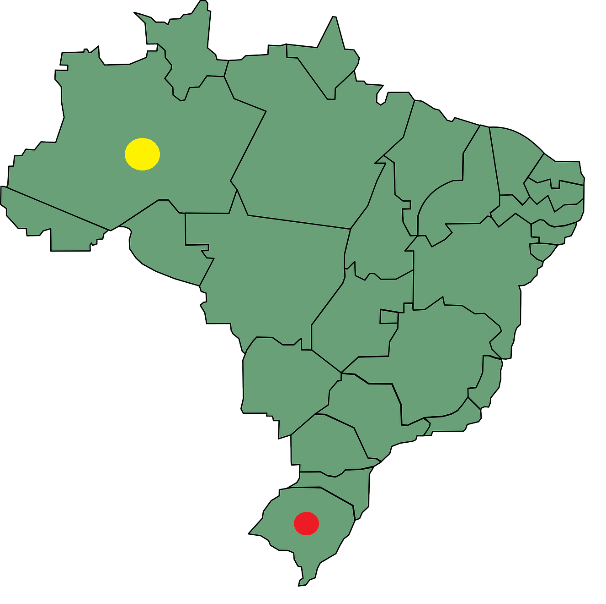
\includegraphics[width=2.73952in,height=2.725in]{./imgSAEB_8_MAT/media/image36.png}

\url{https://pixabay.com/pt/vectors/brasil-mapa-am\%c3\%a9rica-do-sul-estados-23553/}

Inserir um mapa similar a esse, podendo ser alterada as cores e o
estilo, mas que o conteúdo continue o mesmo.

Considerando que a casa de Paulo está demarcada com a esfera vermelha e
a casa de seus pais com a esfera amarela, quantos estados no mínimo
Paulo vai ter que atravessar para ver seus pais?

Deixar o espaço de 2 linhas para resposta.

Resposta: Paulo no mínimo atravessará 4 estados até chegar na casa de
seus pais.

2) A circunferência da terra possui 40~075~km de extensão, suponhamos
que Júlio queria dar uma volta ao mundo em 80 dias com o seu barco, qual
deslocamento diário aproximado que Júlio deverá percorrer para cumprir
seu objetivo?

Considerando que a terra possui 40 075 km de extensão e a viagem deverá
durar no máximo 80 dias, logo:

40 075km : 80 dias =aproximadamente 501 km por dia Júlio deverá navegar.

3) Francisco estava em casa, e resolveu convidar sua namorada para
jantar fora em um famoso restaurante de sua cidade, para ficar mais
fácil de sua namorada encontrar o restaurante Francisco mandou um mapa
da trajetória da sua casa até o restaurante.

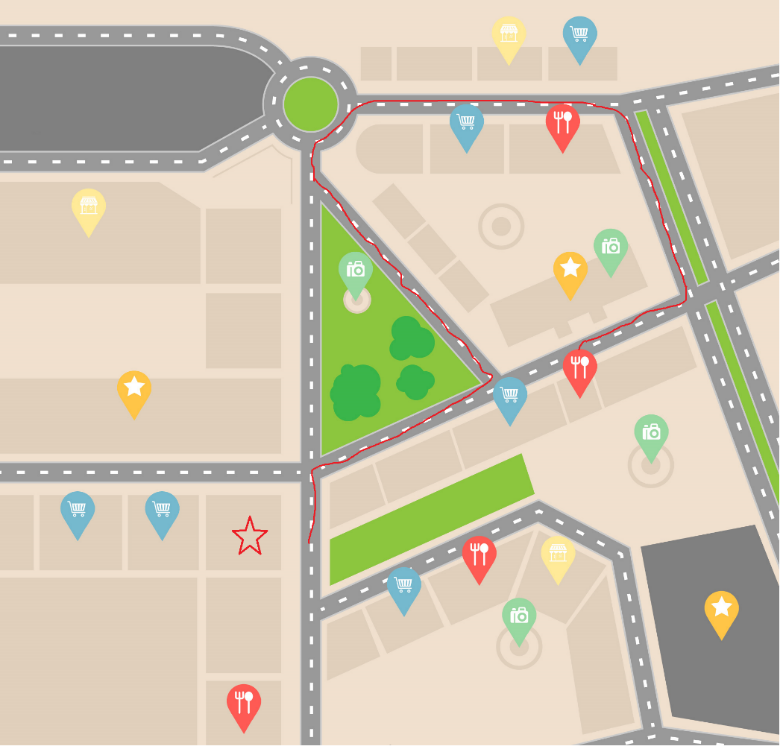
\includegraphics[width=3.55in,height=3.406in]{./imgSAEB_8_MAT/media/image37.png}

\url{https://br.freepik.com/vetores-gratis/mapa-cidade-apartamento-desenho_1107608.htm\#query=mapas\&position=6\&from_view=search\&track=sph}
adaptado.

Inserir um mapa similar a esse, podendo ser alterada as cores e o
estilo, mas que o conteúdo continue o mesmo.

Porem a namorada de Francisco não consegue abrir imagens em seu
telefone, qual outra forma Francisco poderia descrever a trajetória de
sua casa representada por uma estrela vermelha no mapa até o
restaurante?

Deixar o espaço de 3 linhas para resposta.

Reposta: Ao sair da Residência de Francisco, pegue a primeira rua a
direita, depois vire a esquerda, depois entre na rotatória e saia na
primeira saída e siga em frente, depois vire a direita na avenida e
finalmente vire a direita.

4) Em uma tarde de domingo João estava entediado em casa e resolveu dar
um passeio da roda gigante de sua cidade.

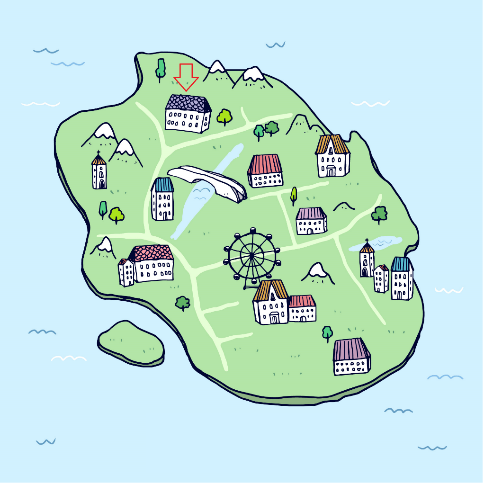
\includegraphics[width=2.2in,height=2.2in]{./imgSAEB_8_MAT/media/image38.png}

\url{https://br.freepik.com/vetores-gratis/mao-desenhado-cidade-mapa-ferris-roda_1106040.htm\#query=mapa\%20feito\%20a\%20m\%C3\%A3o\&position=6\&from_view=search\&track=ais}

Inserir um mapa similar a esse, podendo ser alterada as cores e o
estilo, mas que o conteúdo continue o mesmo.

Considerando que João mora na casa em que a seta está apontada no mapa
qual trajeto da casa de João até a roda gigante podem ser traçados?

Deixar o espaço de 4 linhas para resposta.

Resposta:

João pode Chegar até a roda gigante por dois caminhos, o primeiro
pegando a estrada a direita da sua casa, seguindo nela até virar à
esquerda na estrada da roda gigante.

O segundo caminho é passando pela ponte, no qual João terá que pegar a
estrada a direita de sua casa, atravessar pela ponte e seguir na
estrada, virar à direita após a travessia pela ponte e finalmente virar
à esquerda.

5) Iuri Gagarin, foi o primeiro homem a pisar na lua, considerando que a
distância entre a terra e a lua é de 384~400~km, qual foi o deslocamento
total de Iuri nessa viagem?

Deixar o espaço de 3 linhas para resposta.

Resposta: 384 400 na ida + 384 400 na volta = deslocamento total =768
400 km

6) Lia está fazendo um test drive com um carro de uma concessionária, ao
sair recebeu as seguintes dicas do GPS:

Siga em frente 100m

Vire a esquerda 200m

Vire a esquerda 200 m

Vire a esquerda 200 m

Vire a esquerda 100 m

Ao receber estas informações pode se afirmar que Lia:

Deixar o espaço de 1 linha para resposta.

Voltou a concessionaria.

7) Marcelo e amigos estavam indo para praia, no meio do caminho
perceberam que esqueceram a bagagem em suas casas, assim resolveram
voltar para pega -- las e enfim seguir viagem.

Considerando que a distância de suas casas e a praia seja de 300 km,
qual o deslocamento total de Marcelo e seus amigos até chegarem a praia?

Deixar o espaço de 3 linhas para resposta.

Considerando que já estavam na metade do caminho, percorreram 150 km,
somando mais a viagem completa de 300km, temos que 150 km + 300 km = 450
km

8) Cléber é motorista de uma linha de ônibus de uma metrópole
brasileira, a sua linha anda por 3 bairros diferentes em um percurso
total de 32 km, sabendo que Cléber trabalha das 6 horas da manhã até as
16 horas, e realiza esse percurso 4 vezes, qual o descolamento de Cléber
no trabalho diariamente?

Deixar o espaço de 3 linhas para resposta.

Resposta: 32 km cada percurso, 4 vezes Cléber realiza o percurso por
dia, temos que

4 x 32 km = 128 km por dia.

9) Marina vai ao trabalho de carro, sua jornada de trabalho é de
segunda-feira á sexta-feira, a distância da casa de marina até seu
trabalho é de 12 km, sabendo que seu carro gasta 0, 50 centavos de
gasolina a cada 1 km, qual o valor total que marina gasta com
combustível durante a semana?

Deixar o espaço de 3 linhas para resposta.

Resposta: 12 km para ir e 12 km para voltar = 24 km diários

Logo se a cada 1 km marina gasta 0, 50 centavos temos que em 24 km gasta
12 reais

Contando 5 dias trabalhados na semana 12 x 5 = 60 reais por semana
marina gasta com combustível

10 ) Em um livro infantil um menino sai vagando pelo espaço, de planeta
em planeta caçando novas aventuras , considerando que durante a história
do livro ele tenha visitado 8 planetas e que a distância de entre cada
planeta seja de 10\textsuperscript{5} km qual o deslocamento que o
menino da história realizou?

Deixar o espaço de 3 linhas para resposta.

Resposta Considerando 8 planetas temos que:

8 x 10\textsuperscript{5}

8 x 100 000 = 800 000 km foi o deslocamento.

\colorsec{Treino}

1) Um jogador de Futebol em cada partida corre em média 8 km,
considerando que um campeonato tenha 38 rodadas, e que esse jogador
jogue todas as partidas, qual deslocamento total desse jogador, durante
o campeonato:

a) 8 km por campeonato

b) 38 km por campeonato

c) 30,4 km por campeonato

d) 304 km por campeonato

Resposta: D

Habilidade Saeb:

\begin{itemize}
\tightlist
\item
  Descrever ou esboçar deslocamento de pessoas e/ou de objetos em
  representações bidimensionais (mapas, croquis etc.), plantas de
  ambientes ou vistas, de acordo com condições dadas.
\end{itemize}

A: incorreta, ao considerar que o enunciado pede o valor de km por
partida o aluno pode chegar a essa conclusão.

B: incorreta, o aluno ao considerar a quantidade de rodadas ao invés da
quantidade de km percorridos, pode chegar a esse valor

C: incorreta, ao deslocar erroneamente uma virgula para esquerda o aluno
pode chegar a esse resultado erroneamente.

D: Correta pois

Resposta: 8km x 38 partidas = 304 km por campeonato

2) A velocidade de uma baleia azul pode chegar a 50 km/h, considerando
que uma baleia esteja a navegar pelo mar em sua velocidade máxima, e que
nade por 8 horas ininterruptas, qual o deslocamento total dessa baleia?

a) 40 km

b) 4 000 km

c) 400 km

d) 40 000 km

Resposta: C

Habilidade Saeb:

\begin{itemize}
\tightlist
\item
  Descrever ou esboçar deslocamento de pessoas e/ou de objetos em
  representações bidimensionais (mapas, croquis etc.), plantas de
  ambientes ou vistas, de acordo com condições dadas.
\end{itemize}

A: incorreta, pois esse seria o valor caso o aluno realizasse
incorretamente a multiplicação esquecendo um ``zero'' da expressão.

B: incorreta, pois esse seria o valor caso o aluno realizasse
incorretamente a multiplicação adicionando um ``zero'' na expressão.

C: Correta pois:

50 km -\/-\/-\/-\/-\/-\/-\/-\/-\/-\/-\/-\/- 1 hora

X -\/-\/-\/-\/-\/-\/-\/-\/-\/-\/-\/-\/-\/-\/-\/-\/-\/-\/- 8 horas

50 . 8 = x

400 km essa baleia irá percorrer.

D: incorreta, pois esse seria o valor caso o aluno realizasse
incorretamente a multiplicação adicionando dois ``zeros'' na expressão.

3) Charles é um botânico de renome, e ao sair para realizar pesquisas em
uma floresta acabou se perdendo no meio da mata, Charles também esqueceu
seus equipamentos de navegação em seu laboratório, e a única coisa que
se lembra e que a cidade mais próxima fica ao rumo do pôr sol, para
chegar a cidade mais próxima, para qual sentido Charles deve andar?

a) Norte

b) Sul

c) Leste

d) Oeste

Resposta: D

Habilidade Saeb:

\begin{itemize}
\tightlist
\item
  Descrever ou esboçar deslocamento de pessoas e/ou de objetos em
  representações bidimensionais (mapas, croquis etc.), plantas de
  ambientes ou vistas, de acordo com condições dadas.
\end{itemize}

A: Incorreta, como a questão ela requer que o aluno tenha um
conhecimento básico sobre pontos cardeais o aluno pode considerar
correta esta alternativa caso compreenda que o pôr do sol fique ao Norte
e não ao Oeste.

B: Incorreta, como a questão ela requer que o aluno tenha um
conhecimento básico sobre pontos cardeais o aluno pode considerar
correta esta alternativa caso compreenda que o pôr do sol fique ao sul e
não ao Oeste.

C: Incorreta, como a questão ela requer que o aluno tenha um
conhecimento básico sobre pontos cardeais o aluno pode considerar
correta esta alternativa caso compreenda que o pôr do sol fique ao Leste
e não ao Oeste.

D: Correta

Charles deve seguir rumo ao Oeste.

\section{Módulo 13}

BNCC: EF08MA25.

Habilidades Saeb:

\begin{itemize}
\tightlist
\item
  Identificar os indivíduos (universo ou população-alvo da pesquisa), as
  variáveis e os tipos de variáveis (quantitativas ou categóricas) em um
  conjunto de dados. - Representar ou associar os dados de uma pesquisa
  estatística ou de um levantamento em listas, tabelas (simples ou de
  dupla entrada) ou gráficos (barras simples ou agrupadas, colunas
  simples ou agrupadas, pictóricos, de linhas, de setores, ou em
  histograma). - Inferir a finalidade da realização de uma pesquisa
  estatística ou de um levantamento, dada uma tabela (simples ou de
  dupla entrada) ou gráfico (barras simples ou agrupadas, colunas
  simples ou agrupadas, pictóricos, de linhas, de setores ou em
  histograma) com os dados dessa pesquisa. - Interpretar o significado
  das medidas de tendência central (média aritmética simples, moda e
  mediana) ou da amplitude. - Calcular os valores de medidas de
  tendência central de uma pesquisa estatística (média aritmética
  simples, moda ou mediana). - Resolver problemas que envolvam dados
  estatísticos apresentados em tabelas (simples ou de dupla entrada) ou
  gráficos (barras simples ou agrupadas, colunas simples ou agrupadas,
  pictóricos, de linhas, de setores ou em histograma). - Argumentar ou
  analisar argumentações/conclusões com base nos dados apresentados em
  tabelas (simples ou de dupla entrada) ou gráficos (barras simples ou
  agrupadas, colunas simples ou agrupadas, pictóricos, de linhas, de
  setores ou em histograma). - Explicar/descrever os passos para a
  realização de uma pesquisa estatística ou de um levantamento.
\end{itemize}

Conceitos básicos da Estatística

A Estatística é uma parte da Matemática em que são estudados métodos
para coleta, organização e análise de dados de diferentes áreas, visando
a tomada de decisões. Realizamos uma pesquisa estatística quando
pretendemos estudar alguma característica de determinado conjunto de
elementos, que pode ser de pessoas, resultados, objetos etc. O conjunto
de todos os elementos que têm a característica do interesse da pesquisa
é chamado população. Quando temos muitos elementos na população que
queremos estudar, podemos realizar a pesquisa por meio de uma amostra
que represente essa população.

População é o conjunto de elementos que queremos pesquisar e apresenta
alguma característica comum.

Amostra é um subconjunto, uma parte da população, que apresenta as
mesmas características da população.

Algumas pesquisas necessitam que toda a população seja investigada. Esse
tipo de pesquisa é chamada censitária.

Amostra casual simples

A amostra casual simples é caracterizada por um sorteio aleatório. Os
elementos de uma população podem ser enumerados e, em seguida, sorteados
entre uma quantidade estabelecida previamente.

Amostra sistemática

No caso da amostra sistemática, os elementos da população a ser estudada
já se encontram ordenados. São exemplos: produtos de uma linha de
produção, prontuários médicos, prédios de uma rua etc. Para a seleção
dos elementos que farão parte da amostra, é elaborado um sistema pelo
pesquisador.

Amostra proporcional estratificada

Na amostra estratificada, a população é dividida em subpopulações
chamadas estratos. Esse tipo de amostra é realizado quando outras
características da população devem ser levadas em conta. Por exemplo,
nas pesquisas de intenção de voto para presidente do Brasil, a população
são os eleitores brasileiros, mas a região do país onde reside, o sexo,
a faixa etária e a faixa de renda do eleitor são importantes para essa
pesquisa. Assim, o pesquisador deve selecionar uma amostra aleatória de
cada estrato.

Variáveis

As variáveis são as características que estão sendo analisadas em uma
amostra ou população. Podem assumir valores numéricos e não numéricos.
São classificadas em qualitativas e quantitativas.

Organização dos dados

Para organizar os dados obtidos por meio de uma pesquisa, podemos
construir tabelas e gráficos. O tipo de tabela e de gráfico que vamos
utilizar depende da variável que está sendo analisada

MEDIDAS EM ESTATÍSTICA

Média aritmética

A média aritmética simples de uma série de dados é determinada pela soma
de todos os dados dividida pela quantidade de dados.

Moda

A moda de uma série de dados é determinada pelo valor que apresenta a
maior frequência.

Mediana

A mediana é a medida estatística que divide o conjunto de dados em duas
partes com a mesma quantidade de termos, na qual a primeira parte
apresenta valores menores ou iguais a ela e, na segunda parte, valores
maiores ou iguais a ela.

Questões:

1) Camila uma empresária do ramo de brinquedos estava analisando o
gráfico de vendas do primeiro quadrimestre de 2022,

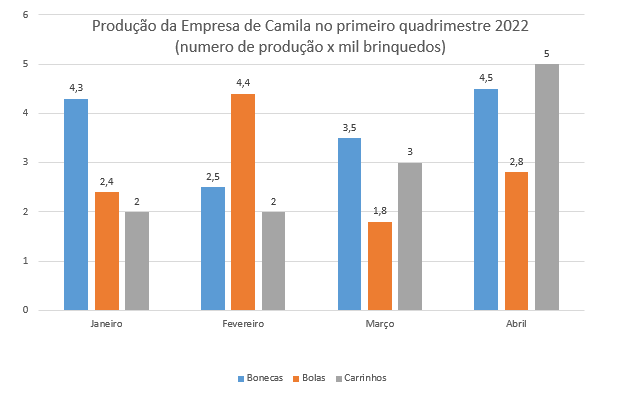
\includegraphics[width=5.90625in,height=3.86458in]{./imgSAEB_8_MAT/media/image39.png}

Inserir um gráfico similar a esse, podendo ser alterada as cores e o
estilo, mas que o conteúdo continue o mesmo.

Ao Analisar o gráfico Camila verificou que:

a) O mês que houve a maior quantidade de brinquedos produzidos foi:

b) O mês que houve a menor quantidade de produção:

c) O brinquedo mais produzido foi:

d) O brinquedo que menos foi produzido foi:

e) Quantos brinquedos ao total a empresa de Camila produziu no primeiro
quadrimestre de 2022?

Deixar o espaço de 1 linha para resposta em cada item acima.

Respostas:

a) Abril

b) Março

c) Os brinquedos mais produzidos foram as Bonecas

d) Os brinquedos menos reproduzidos foram as bolas

e) Realizando a soma dos dados do gráfico obtemos que a empresa de
Camila fabricou ao total de 38 400 brinquedos

2) Ronaldo resolveu colocar em um gráfico todos os custos mensais de sua
casa


\includegraphics[width=5.30833in,height=3.41384in]{./imgSAEB_8_MAT/media/image40.png}

Inserir um gráfico similar a esse, podendo ser alterada as cores e o
estilo, mas que o conteúdo continue o mesmo.

Ao analisar o gráfico responda

a) Ronaldo comprou um ar condicionado que consome muita energia, qual
foi o mês da compra?

b) A filha de Ronaldo Contratou um plano adicional de internet, qual foi
o mês da aquisição?

c) Qual a conta que nunca teve uma grande alta de valor?

d) Em que mês Ronaldo pagou o menor valor de contas na sua casa?

Deixar o espaço de 1 linha para resposta em cada item acima

Respostas:

a) Entre o mês de janeiro e fevereiro

b) No mês de maio

c) A conta de Água

d) Janeiro

3) Poliana está passando por uma reeducação financeira, onde começou a
dividir seus gastos de forma que ainda sobre um dinheiro livre para
aproveitar

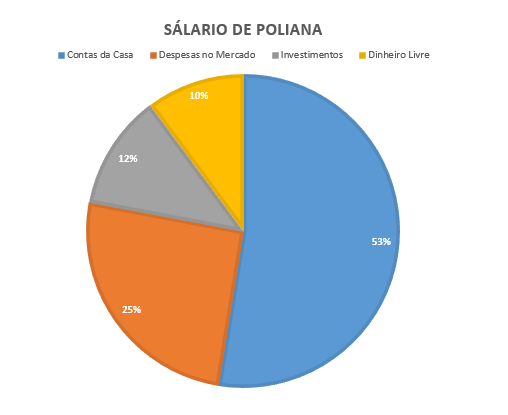
\includegraphics[width=3.65in,height=2.98179in]{./imgSAEB_8_MAT/media/image41.png}

Inserir um gráfico similar a esse, podendo ser alterada as cores e o
estilo, mas que o conteúdo continue o mesmo.

Considerando que o Salário mensal de Poliana é 3 000 reais responda:

a) O valor destinado mensalmente para as contas da casa

b) O valor destinado mensalmente para despesas no mercado

c) O valor destinado mensalmente para investimentos

d) Poliana quer comprar um carro novo no valor de R\$30 000,00 reais, se
Poliana utilizar da parte de investimentos do seu salário, quantos meses
demorará para Poliana comprar o carro?

Deixar o espaço de 1 linha para resposta em cada item acima

Respostas:

a) 3 000 . 0,53 = R\$ 1 590,00

b) 3 000 . 0,25 = R\$ 750,00

c) 3 000 . 0,12 = R\$ 360,00

d) 30 000 : 360 = 84 meses

4) O gráfico abaixo demonstra os títulos relevantes de toda a história
de 4 times de futebol.

{{[}CHART{]}}

Inserir um gráfico similar a esse, podendo ser alterada as cores e o
estilo, mas que o conteúdo continue o mesmo.

Sobre o gráfico podemos afirmar que:

a) O time que mais ganhou campeonatos estaduais foi:

b) Os times que mais ganharam torneios a nível nacional foram:

c) O time que menos ganhou títulos a nível continental foi:

d) Qual o único time que ainda não ganhou nenhum campeonato a nível
mundial:

Deixar o espaço de 1 linha para resposta em cada item acima

Respostas:

a) Time B

b) Times A e C

c) Time B

d) Time C

5) Uma empresa de fornecimento de água contem um controle rigoroso
quanto a quantidade de agua captada pelos seu reservatórios, nos últimos
anos a empresa captou as seguintes informações sobre um dos seu maiores
reservatórios

{{[}CHART{]}}

Inserir um gráfico similar a esse, podendo ser alterada as cores e o
estilo, mas que o conteúdo continue o mesmo.

Todo primeiro dia do Ano está empresa faz um relatório no nível deste
reservatório, observando o gráfico, quais foram os Anos que houve a
maior falta de chuvas?

Deixar o espaço de 1 linha para resposta em cada item acima

Resposta:

Os anos que menos houveram chuvas segundo o gráfico foram em 2014 e
2015.

6) Três amigos resolveram fazer um teste em um clube de futebol, ao
final do teste um analista de desempenho que estava observando os 3
amigos fez um gráfico com algumas características de cada um

{{[}CHART{]}}

Inserir um gráfico similar a esse, podendo ser alterada as cores e o
estilo, mas que o conteúdo continue o mesmo.

Com o relatório do analista em mãos o clube pode tomar algumas
decisões...

a) Caso o clube queira contratar o Jogador mais veloz, qual deve
escolher?

b) Caso o clube queira contratar o Jogador com melhor passe, qual deve
escolher?

c) Caso o clube queira contratar o Jogador mais forte, qual deve
escolher?

d) Considerando que a temporada para o clube seja longa e que o clube
precise contratar o jogar que tenha a maior resistência, qual deve ser a
escolha?

Deixar o espaço de 1 linha para resposta em cada item acima

Respostas:

a) O Clube deve escolher Joãozinho

b) O Clube deve escolher Pedrinho

c) O Clube deve escolher Clebinho

d) O Clube deve escolher Clebinho

7) Uma empresa está realizando uma pesquisa sobre o nível de satisfação
de seus funcionários, para isso, pesquisaram 35 funcionários dos 300
registrados na empresa, com base nas informações anteriores responda:

a) Qual a população dessa pesquisa?

b) Qual a sua amostra?

Deixar o espaço de 1 linha para resposta em cada item acima

Resposta:

a) os 300 funcionários registrados

b) 35 funcionários

8) O quadro mostra algumas notas de matemática de alguns alunos do 8°
ano de uma escola

\begin{longtable}[]{@{}lllll@{}}
\toprule
Notas da disciplina Matemática & & & &\tabularnewline
\midrule
\endhead
Alunos & 1° bimestre & 2° bimestre & 3° bimestre & 4°
bimestre\tabularnewline
Adriana & 7 & 6,5 & 9 & 8\tabularnewline
Bruno & 3 & 5 & 6 & 5\tabularnewline
Carla & 9 & 9 & 8 & 9\tabularnewline
José & 10 & 8 & 8 & 8\tabularnewline
Renata & 5 & 4 & 5 & 3\tabularnewline
\bottomrule
\end{longtable}

Inserir uma tabela similar a essa, podendo ser alterada as cores e o
estilo, mas que o conteúdo continue o mesmo.

Sobre as notas responda:

a) Qual a média aritmética das notas que Adriana obteve nos 4 bimestres?

b) Qual a média aritmética das notas que Bruno obteve nos 4 bimestres?

c) Qual a média aritmética das notas que Carla obteve nos 4 bimestres?

d) Qual a média aritmética das notas que José obteve nos 4 bimestres?

e) Qual a média aritmética das notas que Renata obteve nos 4 bimestres?

f) Sabendo que para ser aprovado na disciplina a média das notas dos 4
bimestres devem ser maior que 6, quais alunos foram aprovados? E Quais
reprovados?

Deixar o espaço de 2 linhas para resposta em cada item acima

Respostas:

a)

7+6,5+9+8 =30,5

30,5 : 4= 7,625

b) 3+ 5+6+5= 19

19:4=4,75

c) 9+9+8+9= 35

35:4= 8,75

d)10+8+8+8=34

34:4= 8,5

e) 5+4+5+3 =17

17:4=4,25

f) Bruno e Renata foram reprovados.

9) Dona Catarina de 82 anos tem 5 irmãs, Genoveva de 79 Anos, Clotilde
de 75, Amélia de 70, Irene de 67 e Tereza de 64, Qual a média de idade
de todas as irmãs?

Deixar o espaço de 2 linhas para resposta

Resposta:

82+79+75+70+67+64= 437

437 : 6 = 72,83

10) Uma professora resolveu fazer uma dinâmica com seus alunos e fez uma
pesquisa com cada um, a pesquisa consistia em apenas 1 pergunta: Qual o
número do seu calçado?

Ao realizar a pesquisa a professora obteve os seguintes dados:

\begin{longtable}[]{@{}llllll@{}}
\toprule
Pesquisa do Número do Calçado de cada Aluno do 8° A & & & &
&\tabularnewline
\midrule
\endhead
35 & 38 & 40 & 42 & 38 & 40\tabularnewline
40 & 38 & 40 & 44 & 40 & 37\tabularnewline
42 & 37 & 42 & 42 & 40 & 44\tabularnewline
40 & 35 & 38 & 40 & 39 & 38\tabularnewline
35 & 38 & 38 & 38 & 44 & 38\tabularnewline
39 & 38 & 38 & 37 & 40 & 37\tabularnewline
\bottomrule
\end{longtable}

Inserir uma tabela similar a essa, podendo ser alterada as cores e o
estilo, mas que o conteúdo continue o mesmo.

Ao observar esses dados Qual a Moda dos números dos calçados dos alunos?

Deixar o espaço de 4 linhas para resposta

Resposta:

Ao observar o quadro temos que

3 Alunos calçam 35

9 alunos calçam 40

4 alunos calcam 42

2 alunos calçam 39

11 alunos calçam 38

3 alunos calcam 44

Logo por método de observação temos que a Moda é os calçados número 38.

Testes:

1) Em um jogo de basquete, os 5 atletas de um time que iniciaram o jogo
tinham respectivamente 2,01m, 1,99m, 2,00m ,2,02 e 1,98m de altura, qual
a estatura média dessa equipe titular?

a) 2,02 m

b) 1,98 m

c) 2 m

d) 10 m

Resposta: C

BNCC: EF08MA25

Habilidade Saeb:

\begin{itemize}
\tightlist
\item
  Calcular os valores de medidas de tendência central de uma pesquisa
  estatística (média aritmética simples, moda ou mediana).
\end{itemize}

A: incorreta, o aluno chegaria a esse resultado, considerando que o
enunciado requer a maior altura da equipe, e não a média aritmética,
chegando a uma conclusão equivocada.

B: incorreta, o aluno chegaria a esse resultado, considerando que o
enunciado requer a menor altura da equipe, e não a média aritmética,
chegando a uma conclusão equivocada.

C: Correta Pois:

Somando a altura dos atletas temos:

2,01 + 1,99 + 2,00 + 2,02 + 1,98 =10

Como são 5 atletas

10 : 5 = 2 metros de altura é a média

D: incorreta, o aluno chegaria a esse resultado, considerando que o
enunciado requer a soma das alturas da equipe, e não a média aritmética,
chegando a uma conclusão equivocada.

2) Um grupo de amigas que frequentam uma academia decidiram compartilhar
o valor de sua última pesagem uma com as outras e chegaram ao seguintes
números:

46kg, 44kg, 49kg, 45kg, 44kg, 48kg, 50kg, 42kg

Qual a mediana do valor do peso em kg dessas amigas?

a) 44kg

b) 45,5kg

c) 46 kg

d) 45kg

Resposta: B

BNCC: EF08MA25

Habilidade Saeb

\begin{itemize}
\tightlist
\item
  Calcular os valores de medidas de tendência central de uma pesquisa
  estatística (média aritmética simples, moda ou mediana).
\end{itemize}

A: incorreta, o aluno chegaria a esse resultado, considerando que o
enunciado requer a moda, e não a média aritmética, chegando a uma
conclusão equivocada.

B: Correta, pois:

Considerando os dois pesos centrais são 46 e 45 kgs Logo 46 + 45 = 91

91 : 2 = 45,5 Alternativa B

C: incorreta, o aluno chegaria a esse resultado, considerando que o
enunciado requer a média aritmética, e não a média aritmética, chegando
a uma conclusão equivocada.

D: o a aluno chegara a esse resultado esquecendo que em casos de
conteúdos pares a mediana deve ser a média entre os dois valores
centrais, no caso ao pegar apenas um valor o aluno chegaria a esse
resultado.

3) Maria caminha todos os dias até seu trabalho, durante uma semana
resolveu cronometrar o tempo que levou de sua casa até seu trabalho:

Segunda-feira: 35 minutos

Terça-feira: 32 minutos

Quarta-feira: 33 minutos

Quinta-feira: 34 minutos

Sexta-feira: 36 minutos

Qual o tempo médio que Maria gasta até chegar no trabalho?

a) 32 minutos

b) 36 minutos

c) 34 minutos

d) 170 minutos

BNCC: EF08MA25

Habilidade Saeb:

\begin{itemize}
\tightlist
\item
  Calcular os valores de medidas de tendência central de uma pesquisa
  estatística (média aritmética simples, moda ou mediana).
\end{itemize}

A: incorreta, o aluno chegaria a esse resultado, considerando que o
enunciado requer o menor tempo gasto, e não a média aritmética, chegando
a uma conclusão equivocada.

B: incorreta, o aluno chegaria a esse resultado, considerando que o
enunciado requer o maior tempo gasto, e não a média aritmética, chegando
a uma conclusão equivocada.

C: correta Pois:

Somando o tempo que Maria gastou na semana temos que:

170 minutos / 5 = média de 34 minutos por dia Maria gasta para chegar ao
trabalho.

D: incorreta, o aluno chegaria a esse resultado, considerando que o
enunciado requer a soma dos tempos que Maria Gasta para ir ao trabalho,
e não a média aritmética, chegando a uma conclusão equivocada.

\section{Módulo 14}

BNCC: EF08MA19 EF08MA20 EF08MA21

Habilidade Saeb:

\begin{itemize}
\item
  Resolver problemas que envolvam medidas de grandezas (comprimento,
  massa, tempo, temperatura, capacidade ou volume) em que haja
  conversões entre unidades mais usuais.
\item
  Resolver problemas que envolvam perímetro de figuras planas.
\item
  Resolver problemas que envolvam área de figuras planas.
\item
  Resolver problemas que envolvam volume de prismas retos ou cilindros
  retos.
\end{itemize}

Área e perímetro de figuras planas

Para calcularmos o perímetro de uma figura plana basta realizar a soma
de todos os lados da figura.

Para o cálculo da área das figuras planas, cada uma tem uma formula
particular:

Veja alguns exemplos de formulas de figuras planas:

Área do quadrado A= l²

Área do triangulo retângulo A= (\frac{b.h}{2})

% REVER
%Área do losango temos que: A=(\frac{\text{D\ .\ d}}{2})=

Área do circulo = (A = \pi r^{2})

Área de um retângulo= A = l . l

Volume de poliedros

Para o cálculo do volume, cada poliedro também tem sua formula
específica para calcular seus respectivos volumes, veja alguns exemplos:

Volume de um cubo V= l . l . l ou l³

Volume de um cilindro V= (\Pi). R² .h

Volume de um paralelepípedo temos que V= l.l.l

\colorsec{Atividades}

1) Considere o cubo abaixo


\includegraphics[width=1.89583in,height=1.27083in]{./imgSAEB_8_MAT/media/image42.png}

Inserir uma imagem similar a essa, podendo ser alterada as cores e o
estilo, mas que o conteúdo continue o mesmo.

a) Qual é a medida de perímetro de uma das faces desse cubo?

b) E qual é a medida de área de uma das faces dele?

c) Qual é a medida de volume do cubo?

Deixar o espaço de 2 linhas para resposta em cada item acima.

Respostas:

a) 4 . 3 = 12cm

b) 3 . 3 = 9cm²

c) 3 . 3 . 3 = 27cm³

2) Determine a medida de área de uma região quadrada sabendo que a
medida de comprimento do lado é de:

a) 8cm

b) 12cm

c) 16 m

d) 20 m

e) 34 m

f) 8 mm

g) 10 mm

h) 25 mm

Deixar o espaço de 2 linhas para resposta em cada item acima.

Respostas:

Considerando a área do quadrado l . l = A

Temos que:

a) 8 . 8 = 64cm²

b) 12 . 12 = 144cm²

c)16 . 16= 256 m²

d)20 . 20 = 400 m²

e)34 . 34= 1156m²

f) 8 . 8 = 64mm²

g) 10 . 10 = 100mm²

h) 25 . 25 = 625 mm²

3) Calcule no caderno a medida de comprimento do lado de uma região
quadrada cuja medida de área é de:

a) 121 cm²

b) 169 cm²

c) 225 cm ²

d) 36m²

e) 324 m²

f) 529 m²

g) 81mm²

h) 729mm²

Deixar o espaço de 2 linhas para resposta em cada item acima.

Respostas

Considerando a área do quadrado l . l = A

Obtemos que l²=A

Logo l = (\sqrt{A})

Aplicando temos que:

a) (\sqrt{121}) = 11cm

b)(\sqrt{169})= 13cm

c)(\sqrt{225})= 15 cm

d)(\sqrt{36})= 6 m

e)(\sqrt{324})= 18 m

f)(\sqrt{529}) = 23 m

g)(\sqrt{81}) = 9 mm

h)(\sqrt{729}) = 27 mm

4) Determine a área de cada figura abaixo

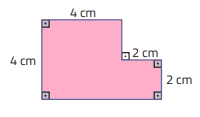
\includegraphics[width=1.65in,height=0.96458in]{./imgSAEB_8_MAT/media/image43.png}a)


\includegraphics[width=1.50833in,height=1.28681in]{./imgSAEB_8_MAT/media/image44.png}b)

Inserir imagens similares a essas, podendo ser alterada as cores e o
estilo, mas que o conteúdo continue o mesmo.

Deixar o espaço de 2 linhas para resposta em cada item acima.

Respostas:

a)

4 . 4 + 2 . 2= A

16+4 =A

A= 20 cm²

b)

\num{6} 3 + 3 . 3 = A

18+9 = A

A= 27cm²

5) Para construir uma caixa com a forma de um bloco retangular sem
tampa, Rosangela recortou uma região poligonal de papelão, como esta
figura, dobrou e colou com fita-crepe. Quantos cm² de papelão ela usou?

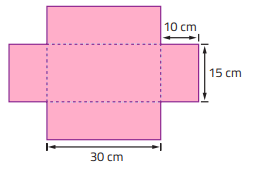
\includegraphics[width=1.98333in,height=1.33255in]{./imgSAEB_8_MAT/media/image45.png}

Inserir uma imagem similar a essa, podendo ser alterada as cores e o
estilo, mas que o conteúdo continue o mesmo.

Deixar o espaço de 2 linhas para resposta

Resposta:

Somando todas as áreas das figuras tracejadas temos que:

10 . 15 + 10 . 15 +10 . 30 + 10 . 30 + 15 . 30= A

150 + 150 + 300 + 300 + 450 = A

A= 1350cm²

6) Determine a área das figuras abaixo

a)


\includegraphics[width=1.26042in,height=1.0625in]{./imgSAEB_8_MAT/media/image46.png}

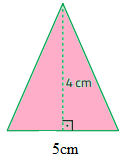
\includegraphics[width=1.39583in,height=1.72917in]{./imgSAEB_8_MAT/media/image47.png}b)

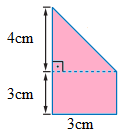
\includegraphics[width=1.375in,height=1.42708in]{./imgSAEB_8_MAT/media/image48.png}c)


\includegraphics[width=1.59375in,height=1.46875in]{./imgSAEB_8_MAT/media/image49.png}d)

Inserir imagens similares a essas, podendo ser alterada as cores e o
estilo, mas que o conteúdo continue o mesmo.

Deixar o espaço de 3 linhas para resposta em cada item acima.

Respostas:

Considerando que a Área do triangulo retângulo é definida por A=
(\frac{b.h}{2}) temos que

a)

A= (\frac{4.8}{2})

A= (\frac{32}{2})

A= 16m²

b)

A=(\frac{\ 2,5.4}{2})

A= (\frac{10}{2})

A= 5 + 5

A =10cm²

c)

A= (\frac{12}{2})

A= 6

6 + 9 = 15 cm²

d)

A= (\frac{4.2}{2})

A= (\frac{8}{2})

A= 4

4+4 + 8.5 =48cm²

7) Ao ler a bula de uma medicação Andreia leu o seguinte dizer: ``Cada
comprimido possui \#\# mm³ dentro de sua capsula'' como não conseguiu
ler pois a escrita estava rasurada, Andreia decidiu fazer suas próprias
medida e obteve:

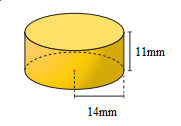
\includegraphics[width=1.88542in,height=1.3125in]{./imgSAEB_8_MAT/media/image50.png}

Inserir uma imagem similar a essa, podendo ser alterada as cores e o
estilo, mas que o conteúdo continue o mesmo.

a)Para saber o volume de medicação dentro da capsula qual formula
Andreia deve utilizar?

b) Considerando (\Pi)=3 qual o volume da capsula?

Deixar o espaço de 2 linhas para resposta em cada item acima.

Respostas:

a) V= (\Pi). R² .h

b) Sendo V= (\Pi). R² .h

temos:

V= 3 . 14 . 11

V= 462 mm³ de medicação

8) Calcule o volume das figuras abaixo

\includegraphics[width=1.94792in,height=0.98958in]{./imgSAEB_8_MAT/media/image51.png}a)

\includegraphics[width=2.08333in,height=1in]{./imgSAEB_8_MAT/media/image52.png}b)

\includegraphics[width=1.92708in,height=1.5625in]{./imgSAEB_8_MAT/media/image53.png}c)

Inserir imagens similares a essas, podendo ser alterada as cores e o
estilo, mas que o conteúdo continue o mesmo.

Deixar o espaço de 3 linhas para resposta em cada item acima.

Resposta:

a)

V= l . l . l

V= 8 . 4 . 3

V= 96cm³

b)

V= l . l . l

V= 4 . 12 . 3

V= 144cm³

144/2

V=72cm³

c)

V= l . l . l

V= 20 . 10 . 15

V = 3000cm³

V= l . l . l

V = 15. 10 .10

V= 1500

1500 + 3000= 4500cm³

9) Marina Resolveu colocar em sua casa uma piscina de 8 metros de
largura, 5 metros de comprimento e 1,5 metros de profundidade, sabendo
que a companhia de agua cobra 0,05 centavos por litro de agua consumido,
quantos reais marina vai gastar para encher completamente essa piscina?

Calculando o volume temos que

V= 8 . 5 . 1,5

V= 60 m³

1m³ = 1000 litros

Deixar o espaço de 2 linhas para resposta

60 m³ = 60 000 litros

1litro custa 0,20 centavos

60 000 . 0,20

= 12000 centavos ou 120 Reais

10) O reservatório de tinta de uma caneta comum tem a forma de um
cilindro. O diâmetro dele tem medida de comprimento de 3 mm e tem 14 cm
de medida de comprimento. Quantos mililitros de tinta essa caneta pode
acomodar? Considere (\Pi)=3,14

Deixar o espaço de 3 linhas para resposta

V= (\Pi). R² .h

V= 3,14 . 1,5² . 140

V= 3,14 . 2,25 . 140

V= 989,1 mm³

Testes

1) Um cano cilíndrico de plástico, tem 70 cm de medida de comprimento e
raio de 6 cm. Qual é a medida de volume de que esse cano comporta?
Considere (\Pi)=3

a) 7 560 cm³

b) 108 cm³

c) 36 cm³

d) 1 260 cm³

Resposta: A

BNCC: EF08MA20

Habilidade Saeb:

\begin{itemize}
\tightlist
\item
  Resolver problemas que envolvam volume de prismas retos ou cilindros
  retos.
\end{itemize}

A: Correta Pois:

V= (\Pi). R² .h

V= 3 . 6² . 70

V= 3 . 36 . 70

V= 7560 cm³

B: Incorreta, o aluno chegaria a esse valor utilizando a formula da área
e não a formula do volume como o enunciado pede.

C: incorreta o aluno chegaria a esse valor calculando o perímetro da
circunferência do cano e não o volume como pede o enunciado.

D: incorreta, o aluno chegaria a esse valor ao esquecer o termo
quadrático, que a formula necessita para obter um valor correto.

2) Vanessa estava pintando um quadro em uma tela retangular de 1 m por
70 cm e começou sua pintura desenhando e colorindo com tinta amarela um
losango de Diagonais 70 cm e 50 cm, no restante do quadro Vanessa
pretende colorir de tinta verde, Qual a área do quadro que falta ser
pintada?

\includegraphics[width=2.95833in,height=1.56526in]{./imgSAEB_8_MAT/media/image54.png}

Inserir uma imagem similar a essa, podendo ser alterada as cores e o
estilo, mas que o conteúdo continue o mesmo.

a) 5 250 cm²

b) 7 000 cm²

c) 1 750 cm²

d) 1 680 cm²

Resposta: A

BNCC: EF08MA19

Habilidade Saeb

\begin{itemize}
\tightlist
\item
  Resolver problemas que envolvam área de figuras planas.
\end{itemize}

A: Correta Pois:

Utilizando a formula da área do losango temos que:

% REVER
% A=(\frac{\text{D\ .\ d}}{2})=

A=(\frac{70\ .\ 50}{2})=

A= (\frac{3500}{2})

A= 1750 cm²

Área do retângulo b.h temos que

A = 100 . 70

A = 7000 cm²

Subtraindo

7000 -- 1750 =5250 cm²

Logo a alternativa correta letra A

B: incorreta, este valor é referente apenas ao valor da área do
retângulo do quadro e não é referente ao valor a ser pintado. Como o
enunciado pede.

C: incorreta, este valor é referente apenas área que já foi pintada e
não a área a ser pintada, como o enunciado pede.

D: incorreta, o aluno chegaria nesse valor, ao não converter o valor em
metros para centímetros, encontrando esse valor erroneamente.

3) Um condomínio resolveu trocar sua caixa e d agua e colocaram uma nova
de formato cilíndrico com diâmetro de base de medida de comprimento de 8
m e altura de medida de comprimento de 5 m.

Qual o volume dessa nova caixa d agua? Considere 
% REVER
% (\text{\ Π})= 3,1
EF08MA20 - Resolver problemas que envolvam volume de prismas retos ou
cilindros retos.

a) 49,6 m³

b) 24,8 m³

c) 62 m³

d) 248 m³

Resposta: D

BNCC: EF08MA20

Habilidade Saeb:

\begin{itemize}
\tightlist
\item
  Resolver problemas que envolvam volume de prismas retos ou cilindros
  retos.
\end{itemize}

A: incorreta, o aluno poderia chegar a esse valor utilizando
erroneamente a formula da área da base, e não a área do volume.

B: incorreta, o aluno poderia chegar a esse valor calculando o perímetro
da base e não o volume total da caixa como o enunciado pede.

C: incorreta, o aluno poderia chegar a essa conclusão ao não observar o
termo quadrático da formula e obter esse resultado erroneamente.

Resposta

V= (\Pi). R² .h

V= 3,1 . 4² . 5

V= 248 m³

Logo alternativa d

\section{Módulo 15}

BNCC: EF08MA22

Habilidade Saeb:

\begin{itemize}
\tightlist
\item
  Resolver problemas que envolvam a probabilidade de ocorrência de um
  resultado em eventos aleatórios equiprováveis independentes ou
  dependentes.
\end{itemize}

A probabilidade (P) de um evento (E) acontecer, a partir de um
experimento aleatório, é dada pela razão entre o número de elementos do
evento e o número de elementos do espaço amostral.

\[P(E)\frac{n(E)}{n(S)}\]

Experimento aleatório

No estudo da probabilidade, um experimento é considerado aleatório se,
mesmo ao repeti-lo um número considerável de vezes, da mesma maneira, o
resultado obtido é sempre imprevisível. O lançamento de um dado e o de
uma moeda são exemplos de experimentos aleatórios, pois em cada
repetição do experimento o resultado obtido não pode ser previsto.

Espaço amostral

Para cada experimento aleatório existe um conjunto de possibilidades de
resultados.

Eventos

Subconjuntos do espaço amostral e são denominadas eventos.

Se o conjunto formado pelos elementos de um evento é vazio, dizemos que
esse evento é impossível.

Quando o número de elementos do evento coincide com o número de
elementos do espaço amostral, o evento é chamado evento certo.

Questões:

1) Em um jogo de tabuleiro Natali precisa de tirar 4 no dado para
conseguir uma bonificação qual é a probabilidade de sair a face com o
número 4 em apenas um lançamento?

Deixar o espaço de 3 linhas para resposta

Resposta:

Para calcular a probabilidade de esse evento ocorrer, determinamos o
número de elementos do espaço amostral e o número de elementos do
evento. Temos:

(P(E)\frac{n(1)}{n(6)}) Logo a chance de Natali tirar o número 4 no
dado e conseguir a bonificação é (\frac{1}{6})

2) Marina está jogando bingo com suas amigas, os números a serem
sorteados nesse bingo vão de 1 a 60 qual a probabilidade de o primeiro
número a ser sorteado ser:

a) Par

b) impar

c) Primo

d) ser múltiplo de 3

e) ser múltiplo de 5

f) ser maior que 50

g) ser menor que 50

Deixar o espaço de 3 linhas para resposta em cada item acima.

Respostas:

a)

(P(E)\frac{n(30)}{n(60)})= (\frac{1}{2}) ou 50\%

b)

(P(E)\frac{n(30)}{n(60)})= (\frac{1}{2}) ou 50\%

c)

(P(E)\frac{n(17)}{n(60)}) =(\frac{17}{60}) ou 28\% aproximadamente

d)

(P(E)\frac{n(20)}{n(60)}) = (\frac{1}{3}) ou 33\% aproximadamente

e)

(P(E)\frac{n(12)}{n(60)})= (\frac{1}{5}) ou 20\%

f)

(P(E)\frac{n(10)}{n(60)})= (\frac{1}{6}) 0u 16\% aproximadamente

g)

(P(E)\frac{n(49)}{n(60)})= (\frac{49}{60}) ou 81\% aproximadamente

3) Sidnei está jogando um jogo de cartas com seus amigos, nesse jogo
existem 4 cartas que são consideradas as mais fortes do jogo, ao pegar
uma carta do baralho qual a chance de Sidnei ter escolhido uma destas
cartas? Considere que o baralho tenha 52 cartas.

Deixar o espaço de 3 linhas para resposta

Resposta:

(P(E)\frac{n(4)}{n(52)})=(\frac{1}{13}) ou 7\%

4)

Gabriela, Carolina, Graziela, Leonardo e Claudio são irmãos, quantas são
as possibilidades de duplas formadas por esses irmãos?

Deixar o espaço de 3 linhas para resposta

Resposta:

(\frac{5!}{3!.2!})=(\frac{120}{6\ .\ 2}) = (\frac{120}{12}) = 10
duplas podem ser formadas

5) João e Maria estão jogando um jogo, no qual consiste em lançar 2
moedas para cima e observar seu resultado após pararem. Para João ganhar
ele precisa que ao lançar as duas moedas, pelo menos uma delas tenha uma
coroa como resultado qual a probabilidade de João vencer o jogo?

Deixar o espaço de 3 linhas para resposta

Resposta:

(P(E)\frac{n(3)}{n(4)})= (\frac{3}{4}) ou 75\%

6) Um parque de diversões resolveu lançar uma promoção para seus
clientes, colocou uma urna contendo 1 200 bolinhas enumeradas de 1 a 1
200, quem encontrasse uma bolinha com o número menor que 10 ganhava um
prêmio, qual a probabilidade de alguém em 1 chance ganhar o prêmio?

Deixar o espaço de 3 linhas para resposta

Resposta:

(P(E)\frac{n(9)}{n(1\ 200)})=(\frac{3}{400}) ou 0,75\%

7) Regiane está indo para uma festa de casamento onde irá usar, um
vestido, um sapato e um colar, Se ela dispõe de 8 vestidos e 12 sapatos
e 3 colares para escolher, de quantos modos diferentes Regiane pode se
vestir?

Deixar o espaço de 3 linhas para resposta

Respostas:

12 .8 . 3= 288 maneiras diferentes

8) Uma professor está montando um provão final para testar o
conhecimento de seus alunos, a prova contem 40 testes, cada um com
quatro alternativas, das quais apenas uma é correta. De quantos maneiras
o gabarito da prova pode ser montado?

Deixar o espaço de 3 linhas para resposta

Respostas:

4 alternativas

40 Questões

Temos que 4\textsuperscript{40}

9) Rita é professora de uma sala de aula do 8° ano com 40 anos, e ao
fazer uma pesquisa na sua sala descobriu que 6 alunos são canhotos.
Certo dia Rita decidiu sortear um livro entre seus alunos, qual a
probabilidade de um aluno canhoto ganhar?

Deixar o espaço de 3 linhas para resposta

Resposta:

(P(E)\frac{n(6)}{n(40)})=(\frac{3}{20})= 15\%

10) Hilária é funcionária de uma empresa de telemarketing, na última
semana do ano haverá um sorteio para saber quem trabalhará em cada dia
da semana, Sabendo se disso qual a probabilidade de Hilária trabalhar no
final de semana? Considerando final de semana sábado e domingo.

Deixar o espaço de 3 linhas para resposta

Resposta:

(P(E)\frac{n(2)}{n(7)})= 28\% aproximadamente

\colorsec{Treino}

1) Em uma fábrica de sapatos houve um defeito com umas das maquinas da
linha de produção, onde após uma pesquisa realizada foi constatado que,
a cada 100 pares produzidos, 4 pares apresentavam algum tipo de defeito,
um inspetor ao selecionar 1 par de sapatos aleatoriamente qual a chance
desse par estar com defeito?

a) 40\%

b) 1\%

c) 4\%

d) 25\%

Resposta: C

BNCC: EF08MA22

Habilidade Saeb:

\begin{itemize}
\tightlist
\item
  Resolver problemas que envolvam a probabilidade de ocorrência de um
  resultado em eventos aleatórios equiprováveis independentes ou
  dependentes
\end{itemize}

A: incorreta, ao converter errado o valor em porcentagem o aluno
chegaria a esse valor deslocando erroneamente a virgula.

B: incorreta, este valor seria o número de calcados a ser pego e não a
porcentagem final provável, logo alternativa incorreta.

C: Correta pois:

(P(E)\frac{n(4)}{n(100)})= 0,04 ou 4\%

D: incorreta, o aluno poderia chegar a essa conclusão ao apenas dividir
o número de calcados totais pelo número de pares de calcados chegando ao
valor descrito na alternativa o que não é o que o enunciado pede.

2) Em um restaurante de comida típica mineira há diversas possibilidades
de cardápio, nele você pode escolher 3 tipos diferentes de guarnições, 4
tipos de carnes, 6 tipos de saladas e 5 tipos de massas. Quantas
possibilidades diferentes de montar o prato um cliente pode ter?

a) 18 possibilidades

b) 72 possibilidades

c) 60 possibilidades

d) 300 possibilidades

Resposta: D

BNCC: EF08MA22

Habilidade Saeb:

\begin{itemize}
\tightlist
\item
  Resolver problemas que envolvam a probabilidade de ocorrência de um
  resultado em eventos aleatórios equiprováveis independentes ou
  dependentes
\end{itemize}

A: incorreta, o aluno pode realizar uma soma ao invés de uma
multiplicação, chegando a esse resultado erroneamente.

b: incorreta, o aluno chegara a esse valor caso esquecer do elemento
``massas'', assim multiplicando os outros fatores chegaria a essa
conclusão.

c: incorreta, o aluno chegara a esse valor caso esquecer do elemento
``saladas'', assim multiplicando os outros fatores chegaria a essa
conclusão.

D: Correta Pois:

Relendo o enunciado temos que:

\num{3} 4 . 6 . 5 = 300

3) Um casal decidiu inovar na escolha do nome de seu novo filho,
resolveram colocar todas as letras do alfabeto em um saquinho, a letra
que fosse sorteada seria a letra inicial do nome.

Em um sorteio em condições justas qual a chance aproximadamente do filho
do casal ter a letra L como inicial do seu nome?

a) 3\%

b) 26\%

c) 1\%

d) 0,3\%

Resposta: A

BNCC: EF08MA22

Habilidade Saeb

\begin{itemize}
\tightlist
\item
  Resolver problemas que envolvam a probabilidade de ocorrência de um
  resultado em eventos aleatórios equiprováveis independentes ou
  dependentes.
\end{itemize}

A: Correta Pois:

(P(E)\frac{n(1)}{n(26)})= 0,03 ou aproximadamente 3\%

B: incorreta o aluno chegaria a essa conclusão ao confundir a quantidade
de letras do alfabeto com a probabilidade do fato acontecer, o que não é
correto.

C: incorreta o aluno chegaria a essa conclusão ao confundir a quantidade
de iniciais, com a probabilidade do fato acontecer, o que não é correto.

D: incorreta, ao deslocar a virgula uma casa para direita o aluno
chegaria a assinalar essa alternativa de forma equivocada.

\section{Simulado 1}

1) O número de ouro é um número\_\_\_\_\_\_\_\_\_\_\_\_\_\_\_,
misterioso e enigmático, presente em uma infinidade de elementos da
natureza na forma de uma razão que é considerada por muitos como a
divina proporção ou razão divina.

Essa razão é o número de ouro, e seu valor é:

(\frac{1 + \ \sqrt{5}}{2}) = 1,6180339887...

Ao observar o enunciado percebe se que falta uma palavra, qual é essa
palavra?

a) Irracional

b) Racional

c) Inteiro

d) Natural

A: correta pois: está faltando a palavra Irracional no texto.

B: incorreta, o aluno pode considerar por semelhança que o número seja
um racional.

C: incorreta, o aluno pode considerar por falta de conhecimento que o
número seja um inteiro.

D: incorreta, o aluno pode considerar por falta de conhecimento prévio
que o número seja de alguma forma natural, devido a todas as respostas
serem conjuntos.

2) Um físico durante seus estudos descobriu que a massa de um elétron
pesa aproximadamente 0,000000000000000000000000000911 g, ao descobrir
tal fato decidiu mandar uma carta para sua mãe demonstrando tal
descoberta, para ocupar o menor espaço possível na carta qual outra
forma que esse número poderia ser reescrito? EF09MA01 Resolver problemas
de adição, subtração, multiplicação, divisão, potenciação ou radiciação
envolvendo número reais, inclusive notação científica

a) 9,11^{.} 10\textsuperscript{-29}

b) 9,11^{.} 10\textsuperscript{-28}

c) 9,11^{.} 10^{-27}

d) 9,11^{.} 10^{-26}

A: incorreta, o aluno ao contar um ``zero'' a mais o aluno chegaria a
esse resultado erroneamente.

B: Correta pois:

Utilizando a notação cientifica temos que:

0,000000000000000000000000000911

30 casas após a virgula, logo é necessário o descolamento do primeiro
número após o 0

Calculando o deslocamento obtém se que o mesmo possui 28 casas logo
temos que

0,000000000000000000000000000911 = 9,11^{.}
10\textsuperscript{-28}

Logo Alternativa B

AlternativaC: incorreta, o aluno ao contar um ``zero'' a menos o aluno
chegaria a esse resultado erroneamente.

D: incorreta, o aluno ao contar dois ``zeros'' a menos o aluno chegaria
a esse resultado erroneamente.

3) Em um festival de Música a capacidade total de público era de 50 000
pessoas, sabendo que compareceram (\frac{99}{100}) do publico total,
Qual foi a capacidade atingida nesse festival? EF08MA05 Representar
frações menores ou maiores que a unidade por meio de representações
pictóricas ou associar frações a representações pictóricas.

a) 49 999

b) 49 500

c) 49 001

d) 4 950

incorreta, o aluno pode chegar à conclusão que de 100-99 = 1, logo ao
tirar também o valor 1 de 50 000, encontraria o resultado correto, o que
não é verídico.

Alternativa: B, Correta pois: Realizando o Cálculo temos que 50 000: 100
= 500

500 . 99 = 49 500 foi o público total.

C: incorreta, o aluno pode considerar retirar 99 do valor de 50 000 e
chegar ao resultado da alternativa descrita, o que significa que o aluno
realizou um calculo incorreto.

D: incorreta, o aluno pode chegar a esse resultado ao invés de
multiplicar o valor de 50 000 por 0,99 , realizar a multiplicação por
0,099.

4) Munir paga R\$ 4,25 por uma passagem do ônibus que usa para ir ao
emprego de enfermeiro Ele ficou sabendo que o preço da passagem terá um
aumento de 12\%. Quanto Munir passará a pagar pela passagem? EF08MA04 -
Resolver problemas que envolvam porcentagens, incluindo os que lidam com
acréscimos e decréscimos simples, aplicação de percentuais sucessivos e
determinação de taxas percentuais.

a) 0,51

b) 3,74

c) 4,37

d) 4,76

A: incorreta, esse seria o acréscimo do valor da passagem, não o valor
final.

B: incorreta, esse seria o valor da passagem caso houvesse 12\% de
desconto e não de acréscimo como o enunciado manda.

C:incorreta, o aluno pode ao invés de calcular a porcentagem, realizar
um soma chegando a essa conclusão.

D: Correta, pois

4,25-\/-\/-\/-\/-\/-\/-\/-\/-\/-\/-\/-\/-\/-\/-\/-\/-\/-\/-\/-\/-\/-100

x-\/-\/-\/-\/-\/-\/-\/-\/-\/-\/-\/-\/-\/-\/-\/-\/-\/-\/-\/-\/-\/-\/-\/-112

4,25 . 112 = x . 100

476= 100x

X= 4,76

5) Frances tem em seu carro R\$ 15,60 em moedas de R\$ 0,10 e de R\$
0,25. Dado que o número de moedas de 25 centavos é o dobro do número de
moedas de 10 centavos, o total de moedas no seu carro é? EF08MA08 -
Resolver problemas que possam ser representados por sistema de equações
de 1º grau com duas incógnitas.

a) 52

b) 26

c) 1 352

d) 78

A: incorreta, o aluno pode considerar que essa seja o valor final do
número de moedas, mas se trata de apenas o valor de um dos termos.

B: incorreta, o aluno pode considerar que essa seja o valor final do
número de moedas, mas se trata de apenas o valor de um dos termos.

C: incorreta, o aluno pode considerar no final do sistemas realizar a
operação de multiplicação ao invés da soma, chegando a essa valor
erroneamente.

D: Correta pois: lendo o enunciado obtemos o seguinte sistema de
equações:

0,25x + 10y = 15,60

X=2y

Logo já conseguimos substituir a 2ª equação na primeira

0,25 .2y + 0,10y =15,60

0,5y + 0,10 y = 15,60

0,60y = 15,60

Y= 26

Como x é o dobro de y, vamos ter que: x=2y = 2. 26 = 52

Logo 52+26= 78 moedas Frances tinha em seu carro, logo alternativa D

6) Arlindo Resolveu presentear sua filha com 2 caixas de tamanhos
diferentes, ambas Arlindo pretende encher com joias, qual a equação que
representa o volume máximo de joias que a filha de Arlindo vai receber
somando o volume das duas caixas? EF08MA10 - Resolver problemas que
envolvam cálculo do valor numérico de expressões algébricas.

\includegraphics[width=2.63333in,height=1.56545in]{./imgSAEB_8_MAT/media/image55.png}

Inserir uma imagem similar a essa contendo os mesmos valores algébricos.

a) X³ + 6x² + 12x +8

b) 21x³ + 62x² + 44x + 8

c) 22x³+ 68x²+56x+

d) 22x³+ 68x²+56x+16

A: incorreta o aluno poderia chegar a essa conclusão chegando apenas ao
valor do volume apenas da primeira caixa.

B: incorreta o aluno poderia chegar a essa conclusão chegando apenas ao
valor do volume apenas da segunda caixa.

C: o aluno chegaria a esse valor calculando incorretamente o ultimo
termo da equação esquecendo de realizar a última parte valor numérico

D: Correta Pois:

Considerando a formula do volume é l\textsuperscript{.}
l\textsuperscript{.} l = volume temos que:

1ª caixa

(x+2)^{.} (x+2)^{.} (x+2)=

(X²+2x+2x+4)\textsuperscript{.} (x+2)=

(x² + 4x +4)^{.} (x+2)=

X³ + 2x² +4x² +8x+4x+8=

X³ + 6x² + 12x +8

2ª caixa

(x+2)^{.(}3x+2)^{.(}7x+2)=

(3x² +2x+6x +4)^{.}(7x+2)=

(3x²+8x +4 )^{.}(7x+2)=

21x³+ 6x² +56x² +16x +28x +8=

21x³ + 62x² + 44x + 8

Somando o valor das 2 caixas temos que

X³ + 6x² + 12x +8 + 21x³ + 62x² + 44x + 8=

22x³+ 68x²+56x+16

7) Josué é estudante de cálculo em uma faculdade de sua cidade, em um
dia que estava em casa Josué resolveu calcular quantos segundos demora
caminhando de um lado para o outro pela casa, e chegou à conclusão que o
tempo em segundos é determinado pela formula t² - 36 = 0 sendo assim
quanto tempo Josué demora para atravessar de um lado para o outro na
casa? EF09MA09 - Resolver problemas que possam ser representados por
equações polinomiais de 2º grau.

a) 36

b) 6

c) 37

d) 2

a: incorreta, este valor representa apenas um dos termos da equação e
não o valor final o aluno pode chegar a assinalar esta resposta por
apenas observar a equação e procurar uma resposta rápida.

b: Correta: pois:

Realizando a operação obtemos:

t² - 36 = 0

t²= (\sqrt{36})

t= ±6

C: incorreta, o aluno pode chegar a esse valor somando todos os termos
da equação o que não é o que o enunciado pede.

D: incorreta, o aluno pode apenas retirar o termo quadrático e cogitar
que essa possa ser a alternativa correta.

8) Helena resolveu visitar seus pais que moram a 455 km de distância de
sua cidade, Helena chegou 7 horas depois que saiu de casa. Qual foi a
velocidade média que helena obteve nesse percurso? EF08MA12 - Resolver
problemas que envolvam variação de proporcionalidade direta ou inversa
entre duas ou mais grandezas, inclusive escalas, divisões proporcionais
e taxa de variação.

a) 65 km/h

b) 7,56 km/h

c) 1,08 km/h

d) 18,05 km/h

A: Correta pois:

% REVER
% Utilizando a razão (\frac{distância}{\text{tempo}}) temos que
% (\frac{455}{7}) = 65km/h

A velocidade média desse carro foi de 65 km/h

B: Incorreta: o aluno pode chegar a essa conclusão caso dividir a
distância pelo valor de 60 minutos ao invés de 7 horas.

C: incorreta, o aluno chegara a essa conclusão confundindo km/h por km/m

D: incorreta o aluno chegara a essa conclusão confundindo km/h por m/s.

9) Considerando a figura, em que ABC é a representação de um triângulo
equilátero, calcule a medida do ângulo x? EF08MA18- Relacionar o número
de vértices, faces ou arestas de prismas ou pirâmides, em função do seu
polígono da base.

\includegraphics[width=0.98958in,height=1.26042in]{./imgSAEB_8_MAT/media/image56.png}

Inserir uma imagem similar a essa.

a) 135°

b) 165°

c) 60°

d) 300°

A:incorreta, o aluno chegaria a essa conclusão realizando apenas a
primeira parte do cálculo esquecendo da figura triangular inserida
abaixo do octógono.

B: Correta pois: Utilizando a Fórmula para obter o valor da figura temos
que:

Por método observativo a figura é um octógono = 8 lados

Utilizando a formula temos que:

(\frac{Ai = \left( 8 - 2 \right)\ \ .\ \ 180}{8}) =

(\frac{Ai = \ 6\ \ .\ \ 180}{8\ }) =

(\frac{Ai = 1080}{8}) = 135°

Agora calculando os ângulos do triangulo

(\frac{Ai = \left( 3 - 2 \right)\ \ .\ \ 180}{3}) =

(\frac{Ai = \ \ \ 180}{3}) = 60°

Por definição temos que 135° + 60 ° - 360° = 165° logo alternativa B

Logo x= 165°

C: resposta incorreta, o aluno pode considera o valor do ângulo interno
do triângulo como resposta, o que é incorreto.

D: o aluno chegaria a esse valor caso não subtraísse também o valor do
ângulo do triângulo chegando a esse valor erroneamente.

10) As medidas dos ângulos de um triângulo são expressas, em grau, por:
3x, 4x +15° e 6x-30° Qual é a medida do maior dos ângulos? EF08MA14 -
Resolver problemas que envolvam relações entre ângulos formados por
retas paralelas cortadas por uma transversal, ângulos internos ou
externos de polígonos ou cevianas (altura, bissetriz, mediana,
mediatriz) de polígonos.

a) 45°

b) 60°

c) 75°

d)180°

A: incorreta, este valor é referente ao menor ângulo do triangulo e não
do maior como o enunciado pede.

B: incorreta, este valor é referente ao segundo maior ângulo do
triangulo e não do maior como o enunciado pede.

C: correta, pois

3x+4x+15+6x-30=180

13x -15=180

13x = 195

X=15

Fazendo a substituição temos que os ângulos são

\% Jorge: Procurar exercício 3. 15 = 45

4. 15 + 15 = 75

6. 15 -- 30 = 60

Logo o ângulo maior é o de valor 75° alternativa c

D: incorreta, este valor é referente ao total da soma dos ângulos do
triangulo e não do maior ângulo como o enunciado pede.

11) Um circuito automobilístico possui 3,337km~de perímetro, uma corrida
neste circuito possui 78 voltas, considerando que um piloto termine a
prova, qual o deslocamento total que ele fará ao todo? Descrever ou
esboçar deslocamento de pessoas e/ou de objetos em representações
bidimensionais (mapas, croquis etc.), plantas de ambientes ou vistas, de
acordo com condições dadas.

a) 260, 286 km

b) 3 415 km

c) 3 259 km

d) 42,78km

A: correta

3,337 x 78 voltas = 260,286 km

B: incorreta, o aluno ao invés de uma multiplicação pode realizar uma
soma em busca da resposta correta, o que não é o que o enunciado pede.

C: incorreta, o aluno ao invés de uma multiplicação pode realizar uma
subtração em busca da resposta correta, o que não é o que o enunciado
pede.

D: incorreta, o aluno ao invés de uma multiplicação pode realizar uma
divisão em busca da resposta correta, o que não é o que o enunciado
pede.

12) Geraldo trabalha como digitador em um fórum de sua cidade, um certo
dia descobriu que digitou 125 000 palavras naquele dia, e assim resolveu
marcar a quantidade de palavras digitadas no resto da semana e obteve os
seguintes números:

1° dia 125 000

2° dia 112 000

3° dia 175 000

4° dia 140 000

5/ dia 101.000

Quantas palavras por dia em média Geraldo digita? EF08MA25 - Calcular os
valores de medidas de tendência central de uma pesquisa estatística
(média aritmética simples, moda ou mediana).

a) 125 000

b) 130 600

c) 112 000

d) 175 000

A: incorreta, este valor é referente apenas ao 1° dia de Geraldo, o
enunciado requer uma média aritmética o que pode levar o aluno a chegar
a assinalar essa alternativa devido a ter este fator na semana de
Geraldo podendo gerar uma confusão entre outras medidas estatísticas.

B: Correta pois:

Somando as palavras digitadas durante os dias temos:

125 000 + 112 000 + 175 000 + 140 000 + 101 000=

653 000 : 6 = 130 600 palavras em média são digitadas por dia.

C: incorreta, este valor é referente apenas ao 2° dia de Geraldo, o
enunciado requer uma média aritmética o que pode levar o aluno a chegar
a assinalar essa alternativa devido a ter este fator na semana de
Geraldo podendo gerar uma confusão entre outras medidas estatísticas.

D: incorreta, este valor é referente apenas ao 3° dia de Geraldo, o
enunciado requer uma média aritmética o que pode levar o aluno a chegar
a assinalar essa alternativa devido a ter este fator na semana de
Geraldo podendo gerar uma confusão entre outras medidas estatísticas.

13) Uma torneira despeja 20 litros de água por minuto. Quanto tempo ela
gasta para encher uma caixa-d'água com a forma de bloco retangular de
lados 2m x 2m x 1m. EF08MA20 - Resolver problemas que envolvam volume de
prismas retos ou cilindros retos.

a) 4 horas

b) 3 horas e 10 minutos

c) 3 horas e 20 minutos

d) 20 minutos

A: incorreta, este valor seria correspondente ao valor do volume e não a
quantidade de tempo, assim o aluno chegaria erroneamente a essa
alternativa.

B: incorreta, ao converter erroneamente o valor de minutos para horas, o
aluno chegaria a essa conclusão.

C: Correta pois:

Para calcular o volume de um bloco retangular temos que V= l.l.l

Logo substituindo temos que:

V= 2.2.1

V=4 m³

4m³ = 4000 litros

20 litros -\/-\/-\/-\/-\/-\/-\/-\/-\/-\/-\/-\/- 1 minuto

4000 litros -\/-\/-\/-\/-\/-\/-\/-\/-\/-\/-\/-\/- x minutos

20 . x = 4000

X = 200 minutos

200 minutos= 3horas e 20 minutos logo alternativa c

D: incorreta, o aluno chegaria a essa conclusão caso inserisse um
``zero'' a menos na expressão chegando a essa conclusão erroneamente.

14) Para brincar de amigo secreto, uma empresa composta por 40
funcionários cortou pedaços idênticos de papel e entregou a cada
funcionário para que escrevesse o próprio nome. Depois, colocaram todos
os pedaços de papel em uma caixa, Paulo será o primeiro a escolher um
papel, qual a chance de Paulo tirar o próprio nome na caixa? EF08MA22 -
Resolver problemas que envolvam a probabilidade de ocorrência de um
resultado em eventos aleatórios equiprováveis independentes ou
dependentes

a) 2,5 \%

b) 1\%

c) 0,25\%

d) 40\%

A: Correta, pois:

(P(E)\frac{n(1)}{n(40)})= 2,5\%

B: incorreta, pois o aluno poderia considerar o número de tentativas ao
invés da probabilidade.

C: incorreta, o aluno chegaria a esse valor deslocando incorretamente a
virgula 1 casa para esquerda.

D: incorreta, o aluno chegaria a essa conclusão ao considerar que o
número de funcionários seja a quantidade de probabilidades o que é
incorreto.

\section{Simulado 2}

1) Qual é o menor número natural que devemos multiplicar pelo número 125
para que o produto seja um número quadrado perfeito?

a) 2

b)3

c)4

d)5

A incorreta, o aluno pode considerar que a palavra quadrado remeta ao
número dois, por semelhança.

B: incorreta, o aluno pode chegar à conclusão que 5³ equivalha a 125
onde se tornaria um quadrado perfeito o que está incorreto.

C: incorreta por considerar que um quadrado possua 4 lados o aluno pode
considerar que tenha algo a ver com o número 4, o que está incorreto.

D,Correta: pois 5 x 125 = 625 e (\sqrt{625}) = 25 logo um quadrado
perfeito.

2) Um empresa de nanotecnologia resolveu inovar e criar o menor chip do
mundo em formato de um quadrado de lados de 2,0^{.} 10
\textsuperscript{-5} cm de comprimento.

Sabendo dessa informação qual a área desse chip em cm²? EF09MA01
Resolver problemas de adição, subtração, multiplicação, divisão,
potenciação ou radiciação envolvendo número reais, inclusive notação
científica

a) 4,0^{.}10\textsuperscript{-10}

b) 2,0\textsuperscript{.} 10\textsuperscript{-5}

c) 4,0^{.} 10\textsuperscript{-5}

d) 2,0\textsuperscript{.}10^{-10}

A: correta pois

Considerando a notação cientifica temos que

2,0^{.} 10^{-5}^{.} 2,0
\textsuperscript{.} 10^{-5} =

Separando os termos

2,0^{.} 2,0 =4,0

10\textsuperscript{-5~.} 10\textsuperscript{-5} =
10\textsuperscript{-10}

Logo temos que a área do Nano chip em cm² é 4,0^{.}
10\textsuperscript{-10}

B: incorreta, ao errar o jogo de sinal na expressão e não realizar a
multiplicação de 2,0 por 2,0, o aluno chegaria a esse resultado,
erroneamente.

C: incorreta, ao errar o jogo de sinal na expressão o aluno chegaria a
esse resultado, erroneamente.

D: Alternativa B: incorreta, ao não realizar a multiplicação de 2,0 por
2,0, o aluno chegaria a esse resultado, erroneamente.

3) Larissa e Leila são irmãs com apenas 1 ano de diferença, ao dividir a
idade de Larissa pela idade de Leila obtemos o valor de 0,933333333...
qual a idade das irmãs? EF08MA05 Determinar uma fração geratriz para uma
dízima periódica.

a) Larissa tem 13 e Leila 12 anos

b) Larissa tem 14 e Leila 15 anos

c) Larissa tem 15 anos e Leila 16 anos

d) Larissa tem 16 anos e Leila 17 anos

A: incorreta, este problema tem 2 soluções possíveis, 1ª realizando um
divisão entre os dois termos, ou encontrando a fração geratriz do
problema, o aluno pode considerar a alternativa correta simplesmente
pelo fato da diferença entre as idades serem apenas de ano, sem realizar
os possíveis cálculos indicados pelo enunciado.

B: Correta, pois:

9,3333333...
-\/-\/-\/-\/-\/-\/-\/-\/-\/-\/-\/-\/-\/-\/-\/-\/-\/-\/-\/-\/-10 x

93,333333...-\/-\/-\/-\/-\/-\/-\/-\/-\/-\/-\/-\/-\/-\/-\/-\/-\/-\/-\/-\/-\/-100x

93,3333333... -- 9,333333333333... = 84

100 x -- 10 x = 90

Logo temos (\frac{84}{90}) simplificando por 6 temos que
(\frac{14}{15}) a idade de Larissa e Leila são respectivamente 14 e 15
anos.

C: incorreta, este problema tem 2 soluções possíveis, 1ª realizando um
divisão entre os dois termos, ou encontrando a fração geratriz do
problema, o aluno pode considerar a alternativa correta simplesmente
pelo fato da diferença entre as idades serem apenas de ano, sem realizar
os possíveis cálculos indicados pelo enunciado.

D: incorreta, este problema tem 2 soluções possíveis, 1ª realizando um
divisão entre os dois termos, ou encontrando a fração geratriz do
problema, o aluno pode considerar a alternativa correta simplesmente
pelo fato da diferença entre as idades serem apenas de ano, sem realizar
os possíveis cálculos indicados pelo enunciado.

4) Manoela está a fim de comprar um vestido para sua festa de formatura
então foi a uma loja e observou que o vestido que queria estava na
promoção com um desconto de 10\%, mas como estava com pressa Manoela
decidiu voltar outro dia;

Ao retornar a loja em outro dia foi informada que o vestido sofreu um
aumento de 10\% em relação ao valor com desconto, pode se dizer que o
valor do vestido em relação ao preço original: EF08MA04 - Resolver
problemas que envolvam porcentagens, incluindo os que lidam com
acréscimos e decréscimos simples, aplicação de percentuais sucessivos e
determinação de taxas percentuais.

a) Não se alterou.

b) Diminuiu 1\%.

c) Aumentou 1\%.

d) Aumentou 79,20\%.

A: incorreta, o aluno chegará a essa conclusão caso não realize os
cálculos necessários, onde achara que por dar 10\% de desconto e depois
adicionar 10\% logo o valor ficaria nulo, o que é incorreto.

B: Correta Pois:

Este problema possui duas formas de solução:

1ª forma:

Valor inicial = x, ao darmos o primeiro desconto temos que x .
(\frac{1}{10}) = (\frac{x}{10})

Ao acrescermos 10\% ao valor dado temos que (\frac{x}{10\ }) .
(\frac{9}{10}) = (\frac{9x}{100}) ou 0,09 ou 9\%, logo o valor final
diminuiu 1\%

2ª forma pelo método da indução, suponhamos que o vestido custe 80 reais
temos que

1° desconto

Utilizando a regra de 3 simples temos que:

80-\/-\/-\/-\/-\/-\/-\/-\/-\/-\/-\/-\/-\/-\/-\/-\/-\/-\/-\/-\/-\/-100

x-\/-\/-\/-\/-\/-\/-\/-\/-\/-\/-\/-\/-\/-\/-\/-\/-\/-\/-\/-\/-\/-\/-\/-90

80 . 90 = 100x

7200 = 100x

X = 72

Com o acréscimo de 10\% temos que

72-\/-\/-\/-\/-\/-\/-\/-\/-\/-\/-\/-\/-\/-\/-\/-\/-\/-\/-\/-\/-\/-100

x-\/-\/-\/-\/-\/-\/-\/-\/-\/-\/-\/-\/-\/-\/-\/-\/-\/-\/-\/-\/-\/-\/-\/-110

72 . 110 = 100x

7920 = 100 x

X = 79,20

Retirando o valor 1da primeira situação do valor da segunda temos que

80 -\/-\/-\/-\/-\/-\/-\/-\/-\/-\/-\/-\/-\/-\/-\/-\/-\/-\/-\/-\/-\/-100

79,20 -\/-\/-\/-\/-\/-\/-\/-\/-\/-\/-\/-\/-\/-\/-\/-\/-\/-\/-\/-\/-x

79,20 . 100 = 80 x

7920 = 80 x

X= 99

Logo o valor do vestido diminuiu 1 \% alternativa letra B

C: incorreta, o aluno pode chegar a essa conclusão devido a semelhança
entre os termos da resposta correta e a resposta incorreta, uma falta de
atenção poderia levar a esse erro.

D: incorreta, o aluno chegaria a essa conclusão caso confundisse o valor
final do produto com a porcentagem correspondente do produto.

5) Comprei 10 Bolas e 15 Bonecas por R\$~800,00. Determine o preço de
cada boneca, sabendo que uma bola e uma boneca custam juntos R\$~60,00.
EF08MA08 - Resolver problemas que possam ser representados por sistema
de equações de 1º grau com duas incógnitas.

a) 20 reais

b) 280 reais

c) 40 reais

d) 60 reais

A: correta Pois:

Determinando com x = bola e y = boneca temos que

10x + 15y = 800

X+y= 60

Isolando o x na segunda equação temos que:

X= 60 -- y

Substituindo a segunda equação na primeira temos:

10(60 -- y) + 15y = 800

600 -- 10y + 15y = 800

5y= 200

Y= 40

Logo se o preço de uma boneca é igual a 40 reais e o preço de uma boneca
e uma bola custam juntos 60 reais

60-40 = 20 o preço da bola é 20 reais logo alternativa A

B: incorreta, o aluno chegaria a essa conclusão caso errasse a troca de
sinal da equação resultante do sistema.

C: incorreta, o aluno pode confundir os resultados entre o preço da bola
e da boneca, assim assinalaria essa alternativa erroneamente.

D: Incorreta: o aluno pode não conseguir deduzir o preço de um brinquedo
do outro chegando a essa conclusão precipitada.

6) Ao jogar um famoso jogo eletrônico, Davi resolveu observar mais cada
peça do jogo, e descobriu que todas as peças do jogo possui pequenos
quadrados de lado (x+6) mm considere que a próxima peça que apareceu na
tela de Davi fosse essa descrita abaixo, qual o valor da área dessa peça
segundo a observação de Davi? EF08MA10 - Resolver problemas que envolvam
cálculo do valor numérico de expressões algébricas.

\includegraphics[width=2.05833in,height=2.16573in]{./imgSAEB_8_MAT/media/image57.png}

Inserir uma imagem similar a essa

a) 16x + 96

b) 4x² + 24x+ 144

c) 4x² + 48x+144

d) x² + 12x + 36

A: incorreta, o aluno poderia ao invés de realizar o cálculo da área
realizar o cálculo do perímetro, chegando a esse resultado incorreto.

B: incorreta, o aluno ao errar a multiplicação no termo ``x''
considerará essa resposta como alternativa correta.

C: Correta pois considerando que cada lado dos quadrados é (x+6) e que a
área do quadrado é l.l temos que:

(x+6) (x+6)=

X² +12x+36

Como temos 4 quadrados na figura:

4 . (X² +12x+36)=

4x² + 48x+144

Logo alternativa correta letra c

D: incorreta, caso o aluno considere calcular apenas 1 quadrado ao invés
da figurar toda chegará a esse resultado erroneamente.

7) Pedro é um professor de matemática em um renomado colégio da cidade,
para representar a sua idade para uma de suas salas de aula Pedro
utilizou a equação

X² - 2 809 = 0, sendo assim qual a idade real de Pedro? EF09MA09 -
Resolver problemas que possam ser representados por equações polinomiais
de 2º grau.

a) 28 anos

b) 19 anos

c) 53 anos

d) 20 anos

A: incorreta, o aluno chegaria a essa conclusão ao pegar apenas uma
parte da equação correspondente e não o resultado final, chegando a uma
resposta equivocada.

B: incorreta, o aluno chegaria a essa conclusão ao somar uma parte da
equação correspondente e não o resultado final, chegando a uma resposta
equivocada.

C: Correta pois:

Realizando as operações obtemos:

X² - 2 809=0

X² = 2 809

X= (\sqrt{2\ 809})

X= 53

Logo Pedro tem 53 anos.

D: incorreta, o aluno chegaria a essa conclusão ao somar os elementos da
equação correspondente e não o resultado final, chegando a uma resposta
equivocada.

8) A China é um dos países mais populosos do mundo, e uma de suas
regiões tem uma população de 7 264 200 habitantes e ocupa uma área de 35
000 km². Qual é a densidade demográfica dessa região? EF08MA12 -
Resolver problemas que envolvam variação de proporcionalidade direta ou
inversa entre duas ou mais grandezas, inclusive escalas, divisões
proporcionais e taxa de variação.

a) 207, 5 Habitantes/km²

b) 4,81 Habitantes/km²

c) 2 075 Habitantes/km²

d) 20 Habitantes/km²

A: correta pois:

Utilizando a razão da densidade demográfica que é

(densidade\ demografica = \frac{número\ de\ pessoas\ }{dimensão\ do\ espaço\ em\ km²})
Temos que:

(densidade\ demografica = \frac{7\ 264\ 200}{35\ 000})

(densidade\ demografica = 207,5\ habitantes)/km²

B: incorreta, o aluno ao invés de realizar a divisão entre número de
pessoas e dimensão do espaço em km² realizar a divisão da dimensão pelo
número de pessoas.

C: incorreta, o aluno pode chegar a esse resultado cortando um ``zero''
a mais da expressão chegando nesse resultado erroneamente.

D: incorreta, o aluno pode chegar a esse resultado cortando um ``zero''
a menos da expressão chegando nesse resultado erroneamente.

9) Um tijolo maciço comum, possui aproximadamente 11 centímetros de
altura e 24 centímetros de comprimento. Para construir uma parede de sua
casa com o tamanho de 7 metros de largura e 4 de altura, Manoel comprou
1500 tijolos, essa quantidade foi suficiente? EF08MA18 -
Construir/desenhar figuras geométricas planas ou espaciais que
satisfaçam condições dadas.

a) Foi suficiente e sobrou 440 Tijolos

b) Foi suficiente e sobrou 1472 Tijolos

c) Não foi suficiente e Faltou 440 Tijolos

d) Manoel comprou tijolos necessários porem não houve sobra.

A: Correta pois:

Calculando a parede da casa obtemos que a mesma possuirá 28m²

Cada tijolo possui 0,11 . 0,24 = 0,0264m² de área

Dividindo 28 : 0,0264 = 1 060 Tijolos

Logo 1500 -- 1060 = 440 tijolos sobraram.

B: incorreta, o aluno chegaria a esse valor caso confundisse área com
perímetro, onde chegaria a esse valor.

C: incorreta, o aluno por meio de indução e não observar o conteúdo da
alternativa pode ser levado a assinala-la, devido aos valores serem
iguais mas o enunciado diferente.

D: incorreta, enunciado inserido para caso o aluno não tenha
conhecimento prévio, procurara a alternativa mais plausível para o
enunciado.

10) Na figura, se AH é a altura e a bissetriz, relativa ao lado BC, do
triângulo ABC. Qual a medida do ângulo x? EF08MA14 - Resolver problemas
que envolvam relações entre ângulos formados por retas paralelas
cortadas por uma transversal, ângulos internos ou externos de polígonos
ou cevianas (altura, bissetriz, mediana, mediatriz) de polígonos.

\includegraphics[width=1.45833in,height=2in]{./imgSAEB_8_MAT/media/image58.png}

Inserir uma imagem similar a essa, podendo ser alterada as cores e o
estilo, mas que o conteúdo continue o mesmo.

a) 136°

b) 22°

c) 44°

d) 68°

A: correta pois:

Utilizando as informações da imagem temos que

68+90 + ângulo BHA = 180

158 + ângulo BHA =180

Ângulo BHA= 22

Logo como há uma bissetriz temos que 22+22= 44°

180°-44°= 136°

Logo alternativa correta letra A

B: incorreta, o aluno chegaria a essa conclusão calculando apenas o
valor do ângulo BHA.

C: incorreta, o aluno chegaria a esse valor calculando apenas o valor da
bissetriz do ângulo.

D: incorreta, o aluno chegaria a essa conclusão considerando o valor de
outro ângulo diferente ao enunciado.

11) Iracema quer realizar uma viagem ao exterior, porem decidiu que o
pais que quer conhecer deve ser um pais que faça divisa com o Brasil,
pois quer fazer essa viagem de carro, sabendo que a distância da sua
cidade a esse pais vizinho é de 1 235 km, e que pretende fazer a viagem
em 30 dias, qual deslocamento diário mínimo Iracema deve fazer para
completar a viagem no prazo. - Descrever ou esboçar deslocamento de
pessoas e/ou de objetos em representações bidimensionais (mapas, croquis
etc.), plantas de ambientes ou vistas, de acordo com condições dadas.

a) 37 km por dia

b) 30 km por dia

c) 41 km por dia

d) 42 km por dia

A: o aluno ao invés de realizar uma divisão dos termos, pode realizar
uma porcentagem chegando a esse resultado erroneamente.

B: incorreta, o aluno pode chegar a essa conclusão confundindo o número
de dias com a quantidade km a ser percorrido.

C: incorreta, o aluno chegaria a essa conclusão desconsiderando as casas
decimais, importante para a solução do problema.

D: Correta pois:

1 235km : 30 dias = 41,16 km diários logo deverá andar com seu carro no
mínimo 42 km por dia.

12) Vicente Resolveu plantar girassóis em sua fazenda, ao pesquisar os
últimos preços da sementes de girassóis obteve os seguintes resultados:
EF08MA25 - Calcular os valores de medidas de tendência central de uma
pesquisa estatística (média aritmética simples, moda ou mediana).

Janeiro: R\$12,25 kg

Fevereiro: R\$13,40 kg

Março: R\$12,95 kg

Abril: R\$11,25 kg

Maio: R\$11,20kg

Junho: R\$12,00 kg

Pode se dizer então que o preço médio nos últimos 6 meses das sementes
de girassol foi? EF09MA22

a) R\$12,17

b) R\$11,20

c) R\$13,40

d) R\$12,12

A: Correta pois:

Somando os meses obtemos: 73,05

73,05 : 6 = 12, 175 logo alternativa correta letra A

B: incorreta, o aluno chegaria a esse resultado, considerando que o
enunciado requer o menor preço, e não a média aritmética, chegando a uma
conclusão equivocada.

C: incorreta, o aluno chegaria a esse resultado, considerando que o
enunciado requer o maior valor, e não a média aritmética, chegando a uma
conclusão equivocada.

D: incorreta, o aluno chegaria a esse resultado, considerando que o
enunciado requer a mediana dos preços, e não a média aritmética,
chegando a uma conclusão equivocada.

13) Mateus Resolveu participar de um famoso campeonato de pipa em sua
cidade, onde a maior pipa vence. Fez então um desenho com as
determinadas metragens.

Para concluir o seu projeto qual a quantidade em m² de folha de seda que
Mateus devera comprar para construir a gigantesca pipa? EF08MA19 -
Resolver problemas que envolvam área de figuras planas.

\includegraphics[width=1.45833in,height=1.63333in]{./imgSAEB_8_MAT/media/image59.png}

Inserir uma imagem similar a essa, podendo ser alterada as cores e o
estilo, mas que o conteúdo continue o mesmo.

Para concluir o seu projeto qual a quantidade em m² de folha de seda que
Mateus devera comprar para construir a gigantesca pipa?

a) 31,68 m²

b) 15,84m²

c) 11,6m²

d) 1,63 m²

A: incorreta, o aluno chegará nesse valor caso considere multiplicar as
duas diagonais em busca do valor da área, sem utilizar a formula
necessária.

B: Correta, pois

Utilizando a formula da área do losango temos que:

% REVER
% A=(\frac{\text{D\ .\ d}}{2})=

A= (\frac{7,2\ .\ 4,4}{2})

A= 15,84 m²

Logo deverá comprar 15,84 m² de folha de seda.

C: Incorreta, o aluno ao invés de utilizar a fórmula do losango para
definir a área, pode somar os valores, e chegar a esse valor
erroneamente.

D: Incorreta, o aluno ao invés de utilizar a fórmula do losango para
definir a área, pode dividir os valores, e chegar a esse valor
erroneamente.

14) Joana está tentando se cadastrar em um site de notícias, Para se
cadastrar ela deve compor uma senha de acesso de 6 caracteres, dos quais
os dois primeiros devem ser vogais e os quatro últimos, algarismos de 0
a 9. Quantas possibilidades de senha diferentes Joana pode criar?
EF08MA22 - Resolver problemas que envolvam a probabilidade de ocorrência
de um resultado em eventos aleatórios equiprováveis independentes ou
dependentes

a) 250 000 possibilidades

b) 25 000 possibilidades

c) 2 500 possibilidades

d) 250 possibilidades

A: Correta pois:

Temos que o número de vogais do nosso alfabeto é 5, logo:

5 . 5 . 10 . 10 . 10 . 10 = 250 000 possibilidades de senhas diferentes.

B: incorreta, ao não considerar ``um elemento multiplicativo 10'' o
aluno chegaria a essa conclusão erroneamente.

C: incorreta, ao não considerar ``dois elementos multiplicativos 10'' o
aluno chegaria a essa conclusão erroneamente.

D: incorreta, ao não considerar ``três elementos multiplicativos 10'' o
aluno chegaria a essa conclusão erroneamente.

\section{Simulado 3}

1) Na sequência de Fibonacci os dois primeiros números são 1 e 1. A
partir daí, cada número é igual à soma dos dois anteriores: 1, 1, 2, 3,
5, 8, 13, 21, ... Qual é o primeiro número dessa sequência que se
escreve com três algarismos? EF09MA04

a) 144

b) 233

c) 377

d) 610

Continuando a calcular a sequência de Fibonacci temos: 13+21 = 34,
34+21= 55, 55+34=89, 89+55 = 144

Logo alternativa A: Correta

B incorreta: pois este valor se refere na realidade ao 2° número acima
de 3 dígitos da sequência de Fibonacci logo não é o que o enunciado
pede.

C incorreta: pois este valor se refere na realidade ao 3° número acima
de 3 dígitos da sequência de Fibonacci logo não é o que o enunciado
pede.

D incorreta: pois este valor se refere na realidade ao 4° número acima
de 3 dígitos da sequência de Fibonacci logo não é o que o enunciado
pede.

2) Em um livro de contos infantis Jonas é um viajante do espaço e está
no planeta Alfa 3301, na história Jonas tem uma canhão de luz em sua
mochila e resolve usa-la para mandar um sinal para a terra, sabendo que
esse planeta se encontra a 6,0^{.} 10\textsuperscript{8}
km da terra e que a velocidade da luz é 3,0^{.}
10\textsuperscript{5} km/s depois de quanto tempo a luz poderia ser
observada por alguém na terra? EF09MA01 Resolver problemas de adição,
subtração, multiplicação, divisão, potenciação ou radiciação envolvendo
número reais, inclusive notação científica

a) 20 segundos

b) 200 segundos

c) 20 000 segundos

d) 2 000 segundos

A: ao considerar dois ``zeros'' a menos em qualquer uma das notações o
aluno chegara a esse resultado erroneamente.

B: ao considerar um ``zero'' a menos em qualquer uma das notações o
aluno chegara a esse resultado erroneamente.

C: ao considerar um ``zero'' a mais em qualquer uma das notações o aluno
chegara a esse resultado erroneamente.

D, correta pois:

Considerando as notações cientificas temos que:

6,0\textsuperscript{.}10\textsuperscript{8} = separando os termos temos
que 6,0 : 3,0 = 2

3,0\textsuperscript{.} 10\textsuperscript{5} e
10\textsuperscript{8}:10\textsuperscript{5}= 10\textsuperscript{3} =
1000

Realizando a operação 2^{.} 1000= 2000

Logo resposta correta d, 2000 segundos.

3) Mario e sua esposa Inês foram viajar para praia ao saírem de sua
cidade encheram o tanque de gasolina mas ao chegarem na metade do
caminho observaram que o tanque de gasolina estava apenas com
(\frac{1}{3}) de gasolina restando, Sabendo que o Tanque de gasolina
comporta 60 litros de gasolina, qual o mínimo de abastecimento que o
casal deve fazer para completar a viagem em segurança? EF08MA05
Representar frações menores ou maiores que a unidade por meio de
representações pictóricas ou associar frações a representações
pictóricas.

a) 20 litros

b) 40 Litros

c) 30 litros

d) 60 litros

A: correta

Se na metade do caminho o tanque estava apenas com (\frac{1}{3}) da
capacidade, temos que em metade da viagem foi consumido (\frac{2}{3})
do tanque, que calculando temos que

60 . (\frac{2}{3}) = (\frac{120}{3}) = 40 litros foram consumidos
Logo sobraram 20 litros

Se em metade do caminho foram consumidos 40 litros, na outra metade
analogamente também serão consumidos 40 litros, e como o tanque já
possui 20 litros que restaram, basta abastecerem apenas mais 20 litros
de gasolina.

B: incorreta, o aluno poderia chegar a essa conclusão ao não compreender
corretamente o enunciado e considerar a quantidade máxima ao invés da
quantidade mínima a ser coloca no tanque de combustível.

C: incorreta, o aluno poderia chegar a essa conclusão ao não compreender
corretamente o enunciado e considerar que a quantidade a ser abastecida,
seria a metade do tanque, devido o enunciado descrever que a conferencia
de abastecimento foi realizada na metade do percurso.

D: incorreta, o aluno pode chegar a essa conclusão caso considere que a
família tenha que abastecer completamente o tanque para concluir a
viagem.

4) Paloma está iniciando uma nova dieta e sabe que 5,6 g de proteína
correspondem a 10\% da sua necessidade diária desse nutriente. Se ela
ingerir 14 g de proteína em uma refeição, que porcentagem da sua
necessidade diária ela estará ingerindo? EF08MA04 - Resolver problemas
que envolvam porcentagens, incluindo os que lidam com acréscimos e
decréscimos simples, aplicação de percentuais sucessivos e determinação
de taxas percentuais.

a) 400\%

b) 14\%

c) 25\%

d) 7,84\%

A: incorreta, o aluno poderia encontrar esse valor multiplicando a regra
de 3 reta ao invés de fazer a multiplicação cruzada.

B: incorreta, 14 na verdade é quantidade de gramas que foi ingerida, o
aluno pode confundir os termos e chegar nessa conclusão erroneamente.

C: correta pois:

x-\/-\/-\/-\/-\/-\/-\/-\/-\/-\/-\/-\/-\/-\/-\/-\/-\/-\/-\/-\/-\/-100

5,6-\/-\/-\/-\/-\/-\/-\/-\/-\/-\/-\/-\/-\/-\/-\/-\/-\/-\/- 10

Temos que:

10x = 5,6 . 100

10x= 560

X= 56 g

Se 56g é o total de proteínas que Paloma necessita no dia, temos que 14g

56-\/-\/-\/-\/-\/-\/-\/-\/-\/-\/-\/-\/-\/-\/-\/-\/-\/-\/-\/-\/-\/-100

14-\/-\/-\/-\/-\/-\/-\/-\/-\/-\/-\/-\/-\/-\/-\/-\/-\/-\/-\/-\/-\/-\/-\/-x

56x = 100 . 14

56x=1400

X=25 \%

D: incorreta, esse valor seria obtido ao calcular incorretamente a regra
de três simples, realizando a multiplicação ao invés da divisão ao fazer
a transição de valores na equação final.

5) Uma pilha de 40 madeiras tem 1,7 m de altura e é formada por madeiras
de 2 cm e de~5~cm~de espessura. Quantas são as madeiras de~2~cm?
EF08MA08 - Resolver problemas que possam ser representados por sistema
de equações de 1º grau com duas incógnitas.

a) 85

b) 10

c) 34

d) 10

A: incorreta, o aluno chegaria a esse valor caso considerar que só há na
pilha madeira de 2cm

B: Correta, pois:

X= quantidade de madeira de 2cm\\
Y= quantidade de madeira de 5cm\\
1,7m=170cm\\
X+Y=40\\
2X+5Y=170\\
Multiplicando a primeira equação por (-2) e somando com a segunda,
fica:\\
-2X-2Y=-80\\
2X+5Y=170\\
Somando: 3Y=90

Y=90/3=30 madeiras de 5cm.\\
X=40-30=10 madeiras de 2cm.

Logo alternativa B.

C: incorreta, o aluno pode considerar essa alternativa correta, caso
entenda que a pilha só possua madeiras de 5cm

D: incorreta, o aluno considerará correta essa questão caso considere
que as madeiras estejam colocadas intercaladas somando 5cm + 2cm,
obtendo 7 cm e dividindo pelo total, logo cálculos equivocados.

6) Ao simplificar a expressão algébrica (x+1)² + (x-1)² + 2(x+1)(x-1)
qual valor obtemos ? EF08MA10 - Resolver problemas que envolvam cálculo
do valor numérico de expressões algébricas.

a) 4x² + 4

b) 4x²

c) 5x²

d) 4x² + 4x

A: incorreta, o aluno errando o sinal de negativo para positivo no termo
2 da expressão final, chegaria a esse resultado erroneamente.

B: Correta pois:

Ao realizarmos as operações lembrando da fatoração por meio da soma de
dois quadrados e da diferença de dois quadrados obtemos que:

(x+1)² + (x-1)² + 2(x+1)(x-1)=

x² + 2x+ 1 + x² -2x +1+ 2(x²-1)=

2x² +2 + 2x² - 2=

4x²

Logo alternativa correta letra b

C: incorreta, ao errar um dos sinais dos termos ``x²'' o aluno chegaria
a esse valor equivocadamente.

D: incorreta, o aluno errando o sinal de negativo para positivo no termo
2x da expressão final, chegaria a esse resultado erroneamente.

7) Alfredo é funcionário de uma empresa de cosméticos, ao pegar seu
holerite percebeu que o seu tempo de serviço em anos é calculado pelo
valor da soma das raízes da equação:

X² - x -- 42 = 0, sendo assim há quantos anos Alfredo já está na
empresa? EF09MA09 - Resolver problemas que possam ser representados por
equações polinomiais de 2º grau.

a) 7 anos

b) 6 anos

c) 42 anos

d) 1 ano

a incorreta: o aluno pode chegar a essa conclusão considerando que o
enunciado pede apenas 1 valor das raízes da equação descrita e não a
soma das raízes, chegando a essa conclusão erroneamente.

b incorreta: o aluno pode chegar a essa conclusão considerando que o
enunciado pede apenas 1 valor das raízes da equação descrita e não a
soma das raízes, chegando a essa conclusão erroneamente.

c incorreta: o aluno pode chegar a essa conclusão considerando que o
enunciado pede o produto das raízes da equação descrita e não a soma das
raízes, chegando a essa conclusão erroneamente.

d: Correta, pois:

Utilizando Bhaskhara temos:

X² - x -- 42 = 0

A=1

B= -1

C= -42

\[\frac{- ( - 1) \pm \sqrt{{( - 1)}^{2} - 4.1.\ ( - 42)}}{2\ .\ 1}\]

\[\frac{1 \pm \sqrt{1 + 168}}{2}\]

\[\frac{1 \pm \sqrt{169}}{2}\]

\[\frac{1 \pm 13}{2}\]

X1=(\frac{1 + 13}{2}) = (\frac{14}{2}) = 7

X2= (\frac{1 - 13}{2})= (\frac{- 12}{2}) = -6

8) A Esmeralda é uma das pedras preciosas mais admiradas em todo o
mundo. Suponha que uma esmeralda tenha 12,2 g de massa e ocupe um volume
de 4 cm³. Qual é a densidade dessa pedra? EF08MA12 - Resolver problemas
que envolvam variação de proporcionalidade direta ou inversa entre duas
ou mais grandezas, inclusive escalas, divisões proporcionais e taxa de
variação.

a) 0,32 g/cm³

b) 16, 2 g/cm³

c) 3,05 g/cm³

d) 8,2 g/cm³

A: incorreta, o aluno pode chegar a esse valor realizando ao invés da
divisão de massa por volume, realizar a divisão volume por massa.

B: incorreta, incorreta, o aluno pode chegar a esse valor realizando ao
invés da divisão de massa por volume, realizar a soma de volume e massa.

C: correta pois:

Utilizando a razão da densidade que é (d = \frac{m}{v}) temos que:

(d = \frac{12,2}{4})

d= 3,05 g/cm³

D: incorreta, incorreta, o aluno pode chegar a esse valor realizando ao
invés da divisão de massa por volume, realizar a subtração de massa por
volume.

9) Juliano Resolveu cercar os animais de sua fazenda para ter o maior
controle sobre eles, então começou a construir uma cerca em formato de
um eneágono regular, para que a construção fique perfeita, qual o valor
correto que cada ângulo interno da cerca deve possuir? EF08MA18-
Relacionar o número de vértices, faces ou arestas de prismas ou
pirâmides, em função do seu polígono da base.

\includegraphics[width=1.575in,height=1.33385in]{./imgSAEB_8_MAT/media/image60.png}

Inserir uma imagem similar a essa.

a) 180°

b) 135°

c) 140°

d) 144°

A: incorreta, o aluno poderia chegar a esse valor esquecendo que a
formula contém uma subtração por 2 no numerador chegando assim a esse
valor erroneamente.

B: incorreta, o aluno chegaria a esse valor, contando 1 lado a menos do
polígono

C: Correta, Pois: Considerando que a formula para calcular cada ângulo
interno de um polígono regular é
(\frac{Ai = \left( n - 2 \right)\ \ .\ \ 180}{n}) temos que:

Polígono que deve ser feito: Eneágono = 9 lados

(\frac{Ai = \left( 9 - 2 \right)\ \ .\ \ 180}{9}) =

(\frac{Ai = 7\ \ \ .\ \ 180}{9}) =

(\frac{Ai = 1260}{9}) = 140° logo alternativa C

D: o aluno chegaria a essa conclusão caso contasse 1 lado a mais na
figura do polígono regular chegando assim a esse resultado erroneamente.

10) Em um triângulo, dois ângulos externos medem 110° e 120°. Os ângulos
internos~desse triângulo medirão, em grau: EF08MA14 - Resolver problemas
que envolvam relações entre ângulos formados por retas paralelas
cortadas por uma transversal, ângulos internos ou externos de polígonos
ou cevianas (altura, bissetriz, mediana, mediatriz) de polígonos.

a) 50°, 60° e 70°

b) 80°, 60° e 70°

c) 50°, 80° e 70°

d) 50°, 60° e 80°

A: Correta, Pois:

Se o 1° ângulo externo mede 110° temos que:

110+ 180=290

360-290= 70°

Já o 2° ângulo mede 120°, logo

120+180= 300

360-300= 60°

Logo 60+70 = 130

130-180= 50

Logo os ângulos internos do triangulo são 50°,60°e 70°

B: incorreta, o aluno chegará a esse resultado casso errar a subtração
no cálculo do 1° ângulo citado no enunciado.

C: incorreta, o aluno chegará a esse resultado casso errar a subtração
no cálculo do 2° ângulo citado no enunciado.

D: incorreta, o aluno chegará a esse resultado casso errar a subtração
no cálculo do 3° ângulo citado no enunciado.

11) Ao entrar em um velho porão abandonado, Bruno descobriu um mapa com
um x marcado, e resolveu ir em busca de um suposto tesouro perdido

\includegraphics[width=2.27099in,height=1.95in]{./imgSAEB_8_MAT/media/image61.png}

\url{https://pixabay.com/pt/vectors/mapa-ilha-mapa-do-tesouro-caminho-7367482/}

Inserir um mapa similar a esse, podendo ser alterada as cores e o
estilo, mas que o conteúdo continue o mesmo.

Considerando que cada tracinho destacado no mapa represente 1 000
metros, Quantos km Bruno andou até chegar na marca do X? - Descrever ou
esboçar deslocamento de pessoas e/ou de objetos em representações
bidimensionais (mapas, croquis etc.), plantas de ambientes ou vistas, de
acordo com condições dadas.

a) 33 km

b) 32km

c) 34km

d) 35km

A: Correta pois

No total são 33 traços, logo 33 x 1 000 = 33 000 ou 33km

B: incorreta, o aluno ao contar 1 traço a menos chegaria a esse valor
erroneamente.

C: incorreta, o aluno ao contar 1 traço a mais chegaria a esse valor
erroneamente.

D: incorreta, o aluno ao contar 2 traços a mais chegaria a esse valor
erroneamente.

12) Rodrigo está realizando uma dieta, reduzindo os carboidratos de sua
comida, Veja o consumo de carboidratos diários de rodrigo durante uma
semana:

Segunda-feira: 35g

Terça-feira: 32g

Quarta-feira:37g

Quinta-feira: 28 g

Sexta-feira: 22 g

Sábado: 40g

Domingo: 33g

Qual a quantidade média aproximadamente em g que rodrigo consumiu nessa
semana? EF08MA25 - Calcular os valores de medidas de tendência central
de uma pesquisa estatística (média aritmética simples, moda ou mediana).

a) 35 g

b) 32 g

c) 37g

d) 32 g

A: incorreta, este valor é apenas referente ao dia de segunda na dieta
de Rodrigo o que pode levar o aluno a assinalar essa alternativa
erroneamente.

B: incorreta, este valor é apenas referente ao dia de terça na dieta de
Rodrigo o que pode levar o aluno a assinalar essa alternativa
erroneamente.

C: incorreta, este valor é apenas referente ao dia de Quarta na dieta de
Rodrigo o que pode levar o aluno a assinalar essa alternativa
erroneamente.

D: Correta pois:

Somando a quantidade de gramas consumida durante a semana obtemos:

35+32+37+28+22+40+33 = 227

227 : 7 = 32, 42 logo alternativa D 32 gramas.

13) A água do mar é salgada e em média, em cada 1 L de água marinha há
cerca de 35 g de sal, ao pegar um copo com o formato cilíndrico de 6 cm
de diâmetro de base e 12 cm de altura com agua do mar, quantas g de sal
esse copo terá? Considere (\Pi)=3 EF08MA20 - Resolver problemas que
envolvam volume de prismas retos ou cilindros retos.

a) 0,324 g

b) 1,134 g

c)11,34g

d) 35 g

A: incorreta, o aluno pode chegar a essa conclusão ao confundir o valor
do volume com o valor da quantidade de gramas de sal no copo, como o
enunciado pede.

B: incorreta, ao inserir um zero a mais na equação o aluno chegaria a
esse valor incorretamente.

C: Correta pois:

V= (\Pi). R² .h

V= 3 . 3² . 12

V= 3 . 9 . 12

V = 324 cm³

1 Litro = 1000 cm³

X = 324 cm³

1000x = 324 . 1

X = (\frac{324}{1000})

X= 0,324 litro

Agora se 1litro de agua marinha contem 35 g de sal temos que

1 -\/-\/-\/-\/-\/-\/-\/-\/- 35

0,324 -\/-\/- -x

x.1 = 35 . 0,324

x= 11,34 g de sal

Logo alternativa C

D: incorreta, o aluno poderia chegar a essa conclusão ao compreender que
o enunciado pede o valor de gramas referente a um litro de agua sem ao
menos realizar os cálculos, chagando a esse valor erroneamente.

14) Na entrada de um festival de música foram distribuídas pulseiras de
cores diferentes para cada área do palco, Quem comprou ingressos para
Área VIP, obteve uma pulseira Vermelha, Quem comprou ingressos para
Arquibancada ganhou uma pulseira Azul e quem comprou ingressos para a
pista ganhou uma pulseira verde, Sabendo que foram vendidos 7 000
ingressos para o setor da pista, 3 000 para o setor de arquibancada e 1
000 ingressos para a área VIP, qual a probabilidade aproximadamente de
selecionar alguém aleatoriamente e essa pessoa estar com a pulseira
vermelha? EF08MA22 - Resolver problemas que envolvam a probabilidade de
ocorrência de um resultado em eventos aleatórios equiprováveis
independentes ou dependentes

a) 63\%

b) 9\%

c) 27\%

d) 91\%

A: incorreta, este seria o valor da probabilidade de encontrar alguém
com a pulseira verde e não a pulseira vermelha como enunciado pede.

B: correta Pois

Somando o público do evento temos que:

7 000 + 3 000 + 1 000= 11 000

Utilizando a fórmula temos que:

(P(E)\frac{n(1\ 000)}{n(11\ 000)}) = (\frac{1}{11}) ou 9\%

C: incorreta, este seria o valor da probabilidade de encontrar alguém
com a pulseira azul e não a pulseira vermelha como enunciado pede.

D: incorreta, esse valor seria a probabilidade de não encontrar alguém
com uma pulseira vermelha, o aluno poderia chegar a essa conclusão
interpretando errado o enunciado.

\section{Simulado 4}

1) Ao calcularmos (\sqrt{3^{3} + 3²}) obtemos como resposta:

A) um número natural 243

b) um número natural 6

c) um número irracional menor que 20

d) A potência 3\textsuperscript{5}

A: incorreta ao não extrair o valor da raiz o aluno pode chegar a essa
conclusão

B: Correta. Ao Calcularmos a operação obtemos o valor 6 que é um número
natural.

C: incorreta, ao calcular as potencias utilizando uma propriedade errada
de potencias, o valor seria um irracional menor que 20, o que estaria
incorreto.

D: incorreta: ao calcular erroneamente a expressão abaixo da raiz
chegaria a esse valor equivocadamente.

2) A medida média da distância entre a Terra e o Sol é de
aproximadamente 1,5\textsuperscript{.}10\textsuperscript{8} ,
considerando que fosse possível chegar ao sol dentro de um foguete, e
que esse foguete estivesse a uma velocidade constante de
2,5\textsuperscript{.} 10\textsuperscript{4} km/h, quantas horas
demoraria para se chegar até o sol? EF09MA01 Resolver problemas de
adição, subtração, multiplicação, divisão, potenciação ou radiciação
envolvendo número reais, inclusive notação científica

a) 10 000 horas

b) 0,6 horas

c) 6 000 horas

d) 60 000 horas

A: incorreta, o aluno pode chegar a essa conclusão caso considerar
apenas a base 10, esquecendo o restante do calculo

B: incorreta Ao realizar o cálculo excluindo a parte de base 10 o aluno
chegaria a esse resultado.

C: correta pois

Considerando as notações cientificas temos que:

1,5\textsuperscript{.}10\textsuperscript{8} = separando os termos temos
que 1,5 : 2,5 = 0,6

2,5\textsuperscript{.} 10\textsuperscript{4} e
10\textsuperscript{8}:10\textsuperscript{4}= 10\textsuperscript{4} =
10000

Realizando a operação 0,6^{.} 10000= 6000

Logo resposta correta C, 6000 horas.

D: ao considerar um ``zero'' a mais em qualquer uma das notações o aluno
chegara a esse resultado erroneamente.

3) Dois maratonistas estavam correndo uma maratona de 30 km , após 40
minutos de prova o maratonista A correu (\frac{5}{16}) do percurso ,
enquanto o corredor B correu (\frac{9}{20}) do percurso , qual a
distancia entre os dois após 40 minutos de prova? EF08MA05 Representar
frações menores ou maiores que a unidade por meio de representações
pictóricas ou associar frações a representações pictóricas.

a) 9,375 km

b) 4,125 km

c) 13,5 km

d) 22,875km

A: incorreta, esse resultado seria obtido caso o aluno apenas calculasse
a quilometragem do primeiro atleta do enunciado

B: correta, pois Calculando o corredor A temos que:

30 : 16= 1,875 . 5 = 9,375

Calculando o Corredor B temos que:

30: 20= 1,5 . 9 = 13,5

Logo

13,5 -- 9,375 = 4,125

C: incorreta, esse resultado seria obtido caso o aluno apenas calculasse
a quilometragem do segundo atleta do enunciado.

D: incorreta, esse resultado seria obtido caso o aluno ao invés de
realizar a diferença entre dois atletas, realizasse a adição.

4) Natalia iniciou uma dieta rigorosa, cortou todos os carboidratos,
frituras e guloseimas de sua alimentação, em 1 mês Natalia reduziu sua
massa corpórea em 5\%, chegando a 57 kg. Quantos quilogramas ela reduziu
de sua massa corpórea no período do regime? EF08MA04 - Resolver
problemas que envolvam porcentagens, incluindo os que lidam com
acréscimos e decréscimos simples, aplicação de percentuais sucessivos e
determinação de taxas percentuais.

a) 5 kg

b) 2,85kg

c) 3 kg

d) 60 kg

A: incorreta, o aluno pode reduzir o imc do enunciado o valor ``5'' ao
invés de 5\% chegando nesse valor erroneamente.

B: incorreta, o aluno chegaria a esse valor caso multiplicasse 57 x 0,05
chegando a esse valor.

C: correta, pois

Utilizando a regra de 3 simples temos que:

X-\/-\/-\/-\/-\/-\/-\/-\/-\/-\/-\/-\/-\/-\/-\/-\/-\/-\/-\/-\/-\/-100

57-\/-\/-\/-\/-\/-\/-\/-\/-\/-\/-\/-\/-\/-\/-\/-\/-\/-\/-\/-\/-\/-\/-\/-95

Logo 95 . x = 5700

X= 60

60 kg -- 57gk = 3kg foi a redução obtida por Natalia.

D: incorreta, esse valor é correspondente ao peso anterior de Natalia, e
não a redução de peso obtida.

5) Duas caixas contêm, conjuntamente, 84~pêssegos. Se fossem tirados
quatro pêssegos de uma das caixas e colocados na outra, ambas ficariam
com o mesmo número de pêssegos. Quantos pêssegos contém cada uma das
caixas? EF08MA08 - Resolver problemas que possam ser representados por
sistema de equações de 1º grau com duas incógnitas.

a) 30 pêssegos em uma caixa e 54 na outra

b) 34 pêssegos em uma caixa e 50 na outra

c) 38 pêssegos em uma caixa e 46 na outra

d) 44 pêssegos em uma caixa e 40 na outra

A: incorreta, o aluno pode considerar a alternativa correta por que
satisfaz a condição de conjuntamente terem 84 pêssegos porem não
satisfaz o segundo passo do enunciado, logo a questão necessita que
ambos os termos estejam de acordo, estando apenas um termo correto não é
suficiente que a alternativa esteja correta.

B: incorreta, o aluno pode considerar a alternativa correta por que
satisfaz a condição de conjuntamente terem 84 pêssegos porem não
satisfaz o segundo passo do enunciado, logo a questão necessita que
ambos os termos estejam de acordo, estando apenas um termo correto não é
suficiente que a alternativa esteja correta.

C: correta pois

Renomeando as caixas por x e y temos o seguinte sistema:

X+ y = 84

x-4 = y+4

Isolando o x na 1ª equação temos que

x= 84-y

Inserindo a 1ª equação na segunda temos

84 -- y -- 4 = y+4

76 = 2y

Y= 38

Logo se em uma das caixas tem 38 pêssegos, analogamente na outra caixa
tem 46 pêssegos. Resposta correta alternativa c

D: incorreta, o aluno pode considerar a alternativa correta por que
satisfaz a condição de conjuntamente terem 84 pêssegos porem não
satisfaz o segundo passo do enunciado, logo a questão necessita que
ambos os termos estejam de acordo, estando apenas um termo correto não é
suficiente que a alternativa esteja correta.

6) Ao chegar em casa Leonardo se deparou com um bilhete em cima de seu
celular:

"A senha do wi fi foi trocada, a nova senha é equação resultante destes
termos:

(a² + 2ab + b²) . 3a²"

Qual a nova senha do wifi da casa de Leonardo? EF08MA10 - Resolver
problemas que envolvam cálculo do valor numérico de expressões
algébricas.

a) 3a\textsuperscript{4}+ 6a³b+ 3a²b²

b) 6a²b+ 9 ab\textsuperscript{4}

c) 5ab\textsuperscript{6}

d) 3a\textsuperscript{4}+ 6a³+ 3a²b²

A: correta, pois

Realizando as operações algébricas temos que:

(a² + 2ab + b²) . 3a² =

3a\textsuperscript{4}+ 6a³b+ 3a²b²

Logo alternativa correta letra a

B: Incorreta, o aluno poderia chegar a essa conclusão somando dois
termos não semelhante na expressão.

C: incorreta, o aluno chegaria a essa conclusão apenas somando os termos
da expressão e não realizando os devidos cálculos necessários.

D: incorreta, o aluno poderia esquecer de adicionar uma letra ``b'' na
expressão devido a quantidade de partes literais que o problema exige,
chegando a essa conclusão.

7) Ao Calcularmos o produto das raízes da equação x² - 2x -- 35= 0
obtemos o deslocamento em metros de um veículo em uma rua deserta, sendo
assim pode se dizer que o motorista: EF09MA09 - Resolver problemas que
possam ser representados por equações polinomiais de 2º grau.

a) Movimentou se para frente 7 metros

b) Movimentou se para trás 35 metros

c) Movimentou se para trás 5 metros

d) Movimentou se para frente 2 metros

A: incorreta, este valor é apenas o resultado de uma das raízes da
equação e não o valor final, o que poderia a levar o aluno assinalar a
essa alternativa erroneamente.

B: Correta pois:

Utilizando Bhaskara temos:

x² - 2x -- 35= 0

A= 1

B= -2

C= -35

\[\frac{- ( - 2) \pm \sqrt{{( - 2)}^{2} - 4.1.( - 35)}}{2\ .\ 1}\]

\[\frac{2 \pm \sqrt{4 + 140}}{2}\]

\[\frac{2 \pm \sqrt{144}}{2}\]

\[\frac{2 \pm 12}{2}\]

X1= (\frac{2 + 12}{2}) = (\frac{14}{2}) = 7

X2 = (\frac{2 - 12}{2}) = (\frac{- 10}{2}) = -5

Multiplicando as raízes obtemos -- 35, logo como o número é negativo
obtemos que o motorista andou para traz 35 metros

C: incorreta, este valor é apenas o resultado de uma das raízes da
equação e não o valor final, o que poderia a levar o aluno assinalar a
essa alternativa erroneamente.

D: incorreta, este valor é apenas o resultado da soma das raízes da
equação e não o valor do produto, o que poderia a levar o aluno
assinalar a essa alternativa erroneamente.

8) Uma construtora resolveu inovar e lançar o maior arranha céu do
Brasil que será construído em uma metrópole. A maquete desse novo
arranha céu foi construída na escala de 1: 390. Sabendo que esse
edifício terá 102 andares e que, em média, cada andar tem 3 m de altura,
determine a medida da altura desse edifício na maquete.

EF08MA12 - Resolver problemas que envolvam variação de proporcionalidade
direta ou inversa entre duas ou mais grandezas, inclusive escalas,
divisões proporcionais e taxa de variação.

a) 411 cm

b) 30 990 cm

c) 0,26 cm

d) 78,46 cm

A: incorreta, o aluno chegará nesse valor caso ao invés de realizar uma
divisão, realizar uma soma dos termos do enunciado.

B: incorreta, o aluno chegará nesse valor caso ao invés de realizar uma
divisão, realizar uma soma no final da expressão.

C: incorreta, o aluno chegará nesse valor caso desconsiderar o valor de
3 metros de altura por andar, realizando apenas a divisão.

D: Correta, pois:

Considerando que o novo prédio terá 96 andares e que cada um possui 3
metros, logo o prédio terá 306 metros de altura.

Utilizando a escala 1: 390 temos que

306 m = 30 600 cm

30 600 / 390 = 78,46 cm.

9) A soma das medidas dos ângulos internos de um polígono regular é
igual a 1 260°. Qual a medida do ângulo externo? EF08MA18- Relacionar o
número de vértices, faces ou arestas de prismas ou pirâmides, em função
do seu polígono da base.

a) 320°

b) 9 °

c) 140°

d) 40°

A: incorreta, o aluno poderia considerar como correta a alternativa ao
somar o valor dos ângulos ao invés de subtrair no final da expressão.

B: incorreta, o aluno poderia considerar esse valor como correto ao
considerar que o número de lados do polígono seja igual ao grau de cada
ângulo.

~Alternativa C: incorreta, o aluno chegaria a esse valor caso invertesse
os valores de ângulos internos e externos chegando a esse resultado
erroneamente.

D: Correta pois:

Si = 180(n -2)

1260 = 180(n - 2)

~1260 : 180 = n - 2

~n = 7 + 2 = 9

~O polígono tem 9 lados.

~O angulo interno:

1260: 9 = 140°

~A soma dos ângulos externos em todo polígono regular é 360°

O angulo interno com o corresponde angulo externo são suplementares
(somam 180°)

Então:

~180 = 140 + Ae

~Ae = 40

~O angulo externo mede 40°

10) Na figura, o ângulo ADC é reto. A medida do ângulo CBD é: EF08MA14 -
Identificar propriedades e relações existentes entre os elementos de um
triângulo (condição de existência, relações de ordem entre as medidas
dos lados e as medidas dos ângulos internos, soma dos ângulos internos,
determinação da medida de um ângulo interno ou externo)

\includegraphics[width=1.68333in,height=1.49462in]{./imgSAEB_8_MAT/media/image62.png}

Inserir uma imagem similar a essa, podendo ser alterada as cores e o
estilo, mas que o conteúdo continue o mesmo.

a) 80°

b) 40°

c) 30°

d) 100°

A: incorreta, o aluno chegaria a essa conclusão caso considerasse apenas
o primeiro cálculo e não o cálculo completo da expressão.

B: o aluno chegaria a esse valor caso não compreendesse corretamente o
que o enunciado pede, e assim escolhendo uma alternativa que o valor
contenha na figura descrita acima.

C: o aluno chegaria a esse valor caso não compreendesse corretamente o
que o enunciado pede, e assim escolhendo uma alternativa que o valor
contenha na figura descrita acima.

D: Correta. Pois:

No triangulo ABD temos que

40+ x + (90-30) = 180

40 + x + 60 =180

100 + x = 180

X = 80

Se o ângulo B = 80 logo:

180 + 80- x =360

X= 100

O ângulo que procuramos tem 100° logo alternativa D

11) A velocidade de um Guepardo pode alcançar 130~km/h, considerando que
um Guepardo em sua velocidade máxima correu atrás de sua presa por 20
minutos, qual foi o deslocamento total em km que esse Guepardo
percorreu? Descrever ou esboçar deslocamento de pessoas e/ou de objetos
em representações bidimensionais (mapas, croquis etc.), plantas de
ambientes ou vistas, de acordo com condições dadas.

Considere 130 km = 36 m/s

a) 2 600 km

b) 43 200 km

c) 43, 2 km

d) 432 km

A: incorreta, ao não realizar a conversão de km/h para m/s o aluno
chegara a esse valor.

B: incorreta, ao não transformar metros em km o aluno chegaria a esse
resultado.

C: Correta pois

Considerando que a velocidade máxima do guepardo foi de 36 m/s e que

20 min = 1 200 segundos

1 200 x 36 = 43 200 metros ou 43,2 km

D: incorreta, ao deslocar a vírgula uma casa a mais o aluno chegaria a
esse resultado erroneamente.

12) Em uma corrida automobilística um piloto obteve as seguintes
velocidades ao passar em diferentes setores da pista:

Ao passar no setor 1 estava em uma velocidade de 280km/h

Ao passar no setor 2 estava em uma velocidade de 290 km/h

Ao passar no setor 3 estava em uma velocidade de 305 km/h

Ao passar pelo setor 4 estava em uma velocidade de 201 km/h

Qual a velocidade média que esse piloto obteve durante essa volta?
EF08MA25 - Calcular os valores de medidas de tendência central de uma
pesquisa estatística (média aritmética simples, moda ou mediana).

a) 280 km/

b) 290km/h

c) 305 km/h

d) 269 km/h

A: incorreta, este valor é referente apenas a velocidade ao passar no
primeiro setor.

B: incorreta, este valor é referente apenas a velocidade ao passar no
segundo setor.

C: incorreta, este valor é referente apenas a velocidade ao passar no
terceiro setor.

D: Correta Pois:

Somando as velocidades nos setores temos: 1076

Dividindo por 4 setores: 269 km/ h foi a velocidade média desse piloto.

13) Para armazenar a gasolina que produz, uma usina possui alguns
reservatórios cilíndricos, entre eles um com medida de capacidade de 600
000 Litros e altura interna medindo aproximadamente 8 m. Qual é a medida
do comprimento do diâmetro interno da base desse reservatório? Considere
(\Pi)=3 EF08MA20 - Resolver problemas que envolvam volume de prismas
retos ou cilindros retos.

a) 5 m

b) 25 m

c) 10 m

d) 316 m

A: Incorreta, o aluno chegaria a essa conclusão colocando como resposta
o valor do raio da base do reservatório e não o diâmetro como o
enunciado pede.

B: incorreta, o aluno chegaria a essa conclusão ao não terminar o
cálculo que a expressão pede, e não realizar a radiciação no final da
expressão.

C: Correta pois:

Iniciamos fazendo a conversão

600 000 litros = 600 m³

V= (\Pi). R² .h

600 = 3 . R² . 8

(\frac{600\ }{8})= 3 . R²

75 = 3 . R²

(\frac{75\ }{3}) = R²

25= R²

(\sqrt{25\ }) =R

R = 5

Logo o diâmetro é 10 m

D: incorreta, o aluno chegaria a essa conclusão ao não realizar a
conversão de litros para m³, onde chegaria a esse valor erroneamente.

14) Um grande supermercado lançou uma promoção, que sortearia uma data
aleatória do ano, Quem fizer aniversário exatamente naquela data
sorteada ganharia para o resto da vida 10\% de desconto em compras
naquele supermercado, qual a chance aproximadamente de uma pessoa ganhar
a promoção. Considere o ano comum com 365 dias. EF08MA22 - Resolver
problemas que envolvam a probabilidade de ocorrência de um resultado em
eventos aleatórios equiprováveis independentes ou dependentes

a) 1\%

b) 27\%

c) 2,7\%

d) 0,27\%

A: incorreta, o aluno poderia considerar este valor como correto ao
confundir o número de chances ao percentual correto.

B: incorreta, ao deslocar a virgula uma casa para esquerda o aluno
chegaria a assinalar essa alternativa de forma equivocada.

C: incorreta, ao deslocar a virgula duas casas para esquerda o aluno
chegaria a assinalar essa alternativa de forma equivocada.

D: Correta pois:

(P(E)\frac{n(1)}{n(365)}) = 0,0027 ou 0,27\%

\end{comment}